%%%%%%%%%%%%%%%%%%%%%%%%%%%%%%%%%%%%%%%%%%%%%%%%%%%%%%%%%%%%%%%%%%%%%%%%%%%%%%%%%%%%%%%%%%%%%%%%%%%
%%%%%%%%%%%%%%%%%%%%%%%%%%%%%%%%%%%%%%%%%%%%%%%%%%%%%%%%%%%%%%%%%%%%%%%%%%%%%%%%%%%%%%%%%%%%%%%%%%%
%%%%%%%%%%%%%%%%%%%%%%%%%%%%%%%%%%%%%%%%%%%%%%%%%%%%%%%%%%%%%%%%%%%%%%%%%%%%%%%%%%%%%%%%%%%%%%%%%%%
%%%%%%%%%%%%%%%%%%%%%%%%%%%%%%%%%%%%%%%%%%%%%%%%%%%%%%%%%%%%%%%%%%%%%%%%%%%%%%%%%%%%%%%%%%%%%%%%%%%

\chapter{Cuadros y figuras adicionales}
\label{apendiceA}

En este apéndice se muestran mayores detalles sobre los resultados obtenidas durante los análisis descritos en el capítulo \ref{ch:metodologia}.
%
Este material fue excluido del texto principal con el fin de agilizar su lectura y enfatizar la interpretación de los resultados en el contexto del PDCL, más que la forma en que fueron calculados.

%Los gráficos \ref{a:cabezas_ctrl} y \ref{a:cabezas_pdcl} representan, esquemáticamente, las derivaciones donde las proporciones de épocas estacionarias son diferentes en MOR y NMOR;, más detalles ver la sección \ref{sec:analisis_epoca}.
%%
%Estos gráficos pueden entenderse como una réplica de la figura \ref{cabeza_new} usando varios tamaños de época.

\section{Total de épocas estacionarias}

En esta subsección se reporta el total de segmentos de PSG clasificados como estacionarios, usando la prueba de PSR.
%
La clasificación se efectuó de manera independiente para todas las derivaciones, y que la misma clasificación se repitió usando diferentes tamaños de ventana; se reportan todos los valores obtenidos.

Adicionalmente se reporta los resultados de aplicar la prueba $\chi^2$ de Pearson para proporciones, usada para verificar si las proporciones de épocas estacionarias durante MOR y NMOR ($\text{p}_{\text{MOR}}$ y $\text{p}_{\text{NMOR}}$) son diferentes.

%\begin{figure}
%\centering
%{\small
%\begin{tabular}{lccccc}
%\toprule
%{\small Tamaño de} & \multicolumn{5}{c}{Grupo CTRL} \\
%    \cmidrule{2-6}
%{\small ventana [s]}    & VCR & MJH & JAE & GHA & MFGR \\
%\midrule
%$30 \times 2^1$ &
%
\includegraphics[width=0.13\textwidth]{./img_art_dfa/cabeza_new_VCR_60.pdf} &
%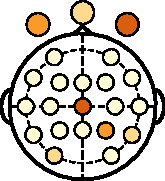
\includegraphics[width=0.13\textwidth]{./img_art_dfa/cabeza_new_MJH_60.pdf} &
%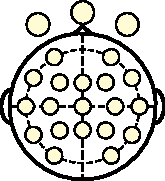
\includegraphics[width=0.13\textwidth]{./img_art_dfa/cabeza_new_JAE_60.pdf} &
%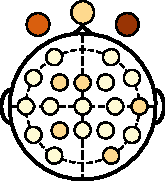
\includegraphics[width=0.13\textwidth]{./img_art_dfa/cabeza_new_GHA_60.pdf} &
%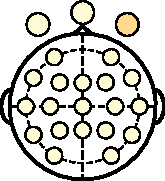
\includegraphics[width=0.13\textwidth]{./img_art_dfa/cabeza_new_MFGR_60.pdf} \\
%\midrule
%$30 \times 2^0$ &
%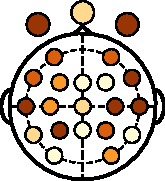
\includegraphics[width=0.13\textwidth]{./img_art_dfa/cabeza_new_VCR_30.pdf} &
%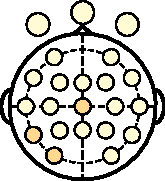
\includegraphics[width=0.13\textwidth]{./img_art_dfa/cabeza_new_MJH_30.pdf} &
%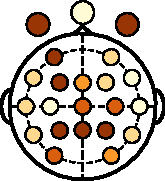
\includegraphics[width=0.13\textwidth]{./img_art_dfa/cabeza_new_JAE_30.pdf} &
%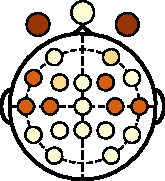
\includegraphics[width=0.13\textwidth]{./img_art_dfa/cabeza_new_GHA_30.pdf} &
%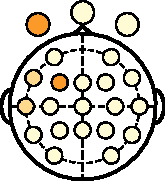
\includegraphics[width=0.13\textwidth]{./img_art_dfa/cabeza_new_MFGR_30.pdf} \\
%\midrule
%$30 \times 2^{-1}$ &
%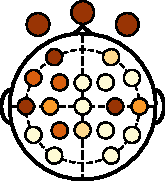
\includegraphics[width=0.13\textwidth]{./img_art_dfa/cabeza_new_VCR_15.pdf} &
%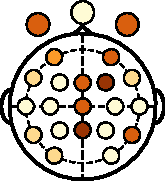
\includegraphics[width=0.13\textwidth]{./img_art_dfa/cabeza_new_MJH_15.pdf} &
%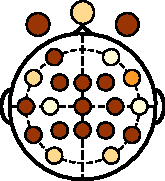
\includegraphics[width=0.13\textwidth]{./img_art_dfa/cabeza_new_JAE_15.pdf} &
%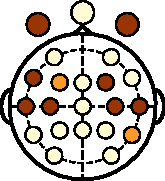
\includegraphics[width=0.13\textwidth]{./img_art_dfa/cabeza_new_GHA_15.pdf} &
%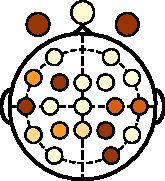
\includegraphics[width=0.13\textwidth]{./img_art_dfa/cabeza_new_MFGR_15.pdf} \\
%\bottomrule
%\end{tabular}\\
%
\includegraphics[scale=.7]{./img_art_dfa/escala.pdf} \\
%}
%\caption{Derivaciones, las cuales la proporción de épocas clasificadas como estacionarias fue significativamente diferente en MOR y NMOR.
%%
%Se han usado diferentes tamaños de ventana.
%%
%La posición de los círculos representan a las derivaciones, en correspondencia con la figura \ref{img:estampa}.}
%\label{a:cabezas_ctrl}
%\end{figure}

%\begin{figure}
%\centering
%{\small
%\begin{tabular}{lccccc}
%\toprule
%{ Tamaño de} & \multicolumn{5}{c}{Grupo PDCL} \\
%    \cmidrule{2-6}
%{ ventana [s]}    & CLO & RLO & RRU & JGZ & AEFP \\
%\midrule
%$30 \times 2^1$ &
%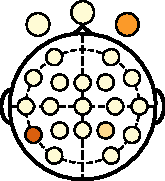
\includegraphics[width=0.13\textwidth]{./img_art_dfa/cabeza_new_CLO_60.pdf} &
%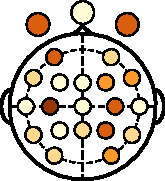
\includegraphics[width=0.13\textwidth]{./img_art_dfa/cabeza_new_RLO_60.pdf} &
%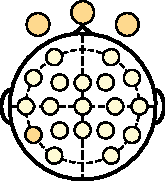
\includegraphics[width=0.13\textwidth]{./img_art_dfa/cabeza_new_RRU_60.pdf} &
%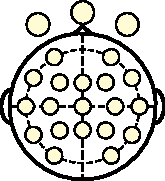
\includegraphics[width=0.13\textwidth]{./img_art_dfa/cabeza_new_JGZ_60.pdf} &
%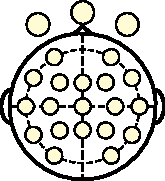
\includegraphics[width=0.13\textwidth]{./img_art_dfa/cabeza_new_AEFP_60.pdf} \\
%\midrule
%$30 \times 2^0$ &
%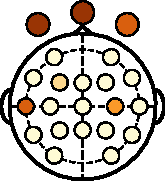
\includegraphics[width=0.13\textwidth]{./img_art_dfa/cabeza_new_CLO_30.pdf} &
%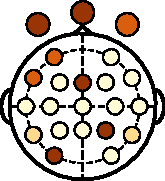
\includegraphics[width=0.13\textwidth]{./img_art_dfa/cabeza_new_RLO_30.pdf} &
%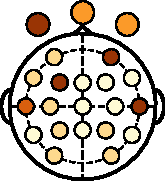
\includegraphics[width=0.13\textwidth]{./img_art_dfa/cabeza_new_RRU_30.pdf} &
%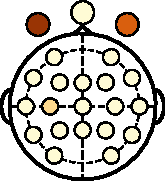
\includegraphics[width=0.13\textwidth]{./img_art_dfa/cabeza_new_JGZ_30.pdf} &
%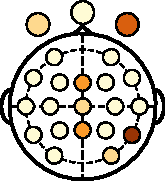
\includegraphics[width=0.13\textwidth]{./img_art_dfa/cabeza_new_AEFP_30.pdf} \\
%\midrule
%$30 \times 2^{-1}$ &
%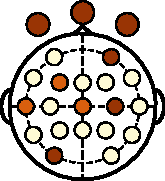
\includegraphics[width=0.13\textwidth]{./img_art_dfa/cabeza_new_CLO_15.pdf} &
%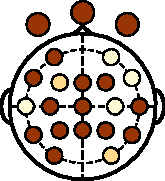
\includegraphics[width=0.13\textwidth]{./img_art_dfa/cabeza_new_RLO_15.pdf} &
%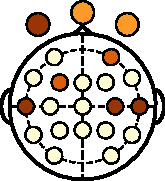
\includegraphics[width=0.13\textwidth]{./img_art_dfa/cabeza_new_RRU_15.pdf} &
%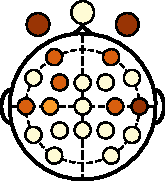
\includegraphics[width=0.13\textwidth]{./img_art_dfa/cabeza_new_JGZ_15.pdf} &
%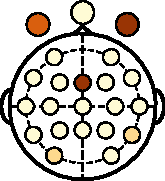
\includegraphics[width=0.13\textwidth]{./img_art_dfa/cabeza_new_AEFP_15.pdf} \\
%\bottomrule
%\end{tabular} \\
%
\includegraphics[scale=.7]{./img_art_dfa/escala.pdf} \\
%}
%\caption{Derivaciones, las cuales la proporción de épocas clasificadas como estacionarias fue significativamente diferente en MOR y NMOR.
%%
%Se han usado diferentes tamaños de ventana.
%%
%La posición de los círculos representan a las derivaciones, en correspondencia con la figura \ref{img:estampa}.}
%\label{a:cabezas_pdcl}
%\end{figure}

%%%%%%%%%%%%%%%%%%%%%%%%%%%%%%%%%%%%%%%%%%%%%%%%%%%%%%%%%%%%%%%%%%%%%%%%%%%%%%%%%%%%%%%%%%%%%%%%%%%
%%%%%%%%%%%%%%%%%%%%%%%%%%%%%%%%%%%%%%%%%%%%%%%%%%%%%%%%%%%%%%%%%%%%%%%%%%%%%%%%%%%%%%%%%%%%%%%%%%%

\begin{SidewaysTable}
\centering
\caption[Épocas estacionarias y comparación de proporciones, MJH (1/2)]{ Épocas estacionarias según tamaño de ventana, y comparación de sus proporciones entre etapas de sueño; participante MJH (1/2)}
{
\begin{tabular}{lrrclrrclrrclrrc}
\toprule
     & \multicolumn{3}{l}{E = 0.9375 s} &  & \multicolumn{3}{l}{E = 1.875 s} &  & \multicolumn{3}{l}{E = 3.75 s} &  & \multicolumn{3}{l}{E = 7.5 s} \\ 
\cmidrule{2-4} \cmidrule{6-8} \cmidrule{10-12} \cmidrule{14-16}
 & \multicolumn{1}{c}{N+W} & \multicolumn{1}{c}{R} & \multicolumn{1}{c}{$p$} &  & \multicolumn{1}{c}{N+W} & \multicolumn{1}{c}{R} & \multicolumn{1}{c}{$p$} &  & \multicolumn{1}{c}{N+W} & \multicolumn{1}{c}{R} & \multicolumn{1}{c}{$p$} &  & \multicolumn{1}{c}{N+W} & \multicolumn{1}{c}{R} & \multicolumn{1}{c}{$p$} \\
\midrule
Fp2   & 19401     & 2495     & ****    &  & 10125     & 1249    & ****    &  & 4664     & 559     & ****    &  & 1710     & 209    & *       \\
Fp1   & 19529     & 2451     & ****    &  & 10308     & 1229    & ****    &  & 4593     & 551     & ****    &  & 1626     & 201    &         \\
F8    & 19241     & 2762     &         &  & 10434     & 1396    & **      &  & 4930     & 644     & *       &  & 1844     & 266    &         \\
F7    & 18978     & 2679     &         &  & 10580     & 1406    & ***     &  & 5075     & 653     & ***     &  & 1900     & 258    &         \\
F4    & 18211     & 2609     &         &  & 10331     & 1539    & ****    &  & 4970     & 755     & ***     &  & 1908     & 333    & ****    \\
F3    & 18546     & 2665     &         &  & 10494     & 1553    & ****    &  & 5093     & 806     & ****    &  & 1983     & 334    & ****    \\
T4    & 19982     & 2935     & ****    &  & 10866     & 1594    & ***     &  & 5212     & 778     & **      &  & 1981     & 314    & **      \\
T3    & 18556     & 2628     &         &  & 10457     & 1501    &         &  & 5190     & 790     & ****    &  & 2057     & 342    & ****    \\
C4    & 18566     & 2735     & ****    &  & 10709     & 1605    & ****    &  & 5284     & 814     & ****    &  & 2100     & 342    & ****    \\
C3    & 18236     & 2575     &         &  & 10553     & 1522    &         &  & 5194     & 798     & ****    &  & 2083     & 333    & ***     \\
T6    & 18521     & 2696     & **      &  & 10815     & 1581    & **      &  & 5362     & 827     & ****    &  & 2138     & 364    & ****    \\
T5    & 18274     & 2372     & ****    &  & 10160     & 1332    & ****    &  & 5297     & 790     & **      &  & 2205     & 368    & ****    \\
P4    & 18330     & 2709     & ****    &  & 10811     & 1599    & ****    &  & 5228     & 819     & ****    &  & 2087     & 336    & ***     \\
P3    & 18336     & 2558     &         &  & 10665     & 1519    &         &  & 5260     & 796     & ****    &  & 2107     & 334    & ***     \\
O2    & 16418     & 2228     &         &  & 10371     & 1469    &         &  & 5313     & 809     & ****    &  & 2192     & 371    & ****    \\
O1    & 17477     & 2402     &         &  & 10431     & 1407    & *       &  & 5519     & 822     & ***     &  & 2326     & 376    & ****    \\
FZ    & 17630     & 2349     & ***     &  & 10375     & 1515    & *       &  & 5070     & 804     & ****    &  & 1998     & 352    & ****    \\
CZ    & 17430     & 2271     & ****    &  & 10255     & 1467    &         &  & 5144     & 776     & ***     &  & 2041     & 344    & ****    \\
PZ    & 17775     & 2559     &         &  & 10683     & 1551    & *       &  & 5359     & 800     & ***     &  & 2176     & 343    & ***     \\
LOG   & 13116     & 1524     & ****    &  & 8658      & 1122    & ****    &  & 5146     & 608     & ****    &  & 2495     & 292    & ****    \\
ROG   & 17253     & 2493     &         &  & 10092     & 1400    &         &  & 5650     & 734     & ****    &  & 2544     & 313    & ****    \\
EMG   & 18803     & 1533     & ****    &  & 8600      & 697     & ****    &  & 3743     & 293     & ****    &  & 1551     & 204    &         \\
\textbf{Total} & 28987     & 4055     &         &  & 14493     & 2031    &         &  & 7246     & 1016    &         &  & 3623     & 508    &         \\ 
\bottomrule
\end{tabular}
\begin{tabular}{p{18cm}}
E=tamaño de ventana; N+W=NMOR y vigilia; R=MOR; $p$, significancia de la prueba $\chi^{2}$ de Pearson entre las proporciones de ventanas estacionarias en N+W y R: *=0.05, **=0.01, ***=0.005, ****=0.001
\end{tabular}
}
\end{SidewaysTable}
\begin{SidewaysTable}
\centering
\caption[Épocas estacionarias y comparación de proporciones, MJH (2/2)]{ Épocas estacionarias según tamaño de ventana, y comparación de sus proporciones entre etapas de sueño; participante MJH (2/2)}
{
\begin{tabular}{lrrclrrclrrclrrc}
\toprule
     & \multicolumn{3}{l}{E = 15 s} &  & \multicolumn{3}{l}{E = 30 s} &  & \multicolumn{3}{l}{E = 60 s} &  & \multicolumn{3}{l}{E = 120 s} \\ 
\cmidrule{2-4} \cmidrule{6-8} \cmidrule{10-12} \cmidrule{14-16}
 & \multicolumn{1}{c}{N+W} & \multicolumn{1}{c}{R} & \multicolumn{1}{c}{$p$} &  & \multicolumn{1}{c}{N+W} & \multicolumn{1}{c}{R} & \multicolumn{1}{c}{$p$} &  & \multicolumn{1}{c}{N+W} & \multicolumn{1}{c}{R} & \multicolumn{1}{c}{$p$} &  & \multicolumn{1}{c}{N+W} & \multicolumn{1}{c}{R} & \multicolumn{1}{c}{$p$} \\
\midrule
Fp2 & 531  & 67  &      &  & 139 & 12  &   &  & 31  & 2  &   &  & 3   & 1  &  \\
Fp1 & 521  & 58  &      &  & 135 & 11  &   &  & 34  & 4  &   &  & 3   & 0  &  \\
F8  & 623  & 89  &      &  & 187 & 22  &   &  & 48  & 7  &   &  & 9   & 2  &  \\
F7  & 670  & 84  &      &  & 209 & 23  &   &  & 56  & 5  &   &  & 11  & 3  &  \\
F4  & 640  & 124 & **** &  & 196 & 32  &   &  & 58  & 12 &   &  & 13  & 1  &  \\
F3  & 681  & 118 & *    &  & 206 & 37  &   &  & 56  & 10 &   &  & 16  & 1  &  \\
T4  & 662  & 121 & ***  &  & 203 & 34  &   &  & 48  & 11 &   &  & 10  & 3  &  \\
T3  & 765  & 131 & *    &  & 245 & 49  & * &  & 72  & 14 &   &  & 17  & 5  &  \\
C4  & 726  & 128 & **   &  & 225 & 29  &   &  & 62  & 9  &   &  & 15  & 2  &  \\
C3  & 741  & 132 & ***  &  & 226 & 35  &   &  & 61  & 16 &   &  & 17  & 2  &  \\
T6  & 754  & 138 & **** &  & 240 & 40  &   &  & 76  & 16 &   &  & 20  & 4  &  \\
T5  & 818  & 143 & ***  &  & 239 & 48  & * &  & 54  & 12 &   &  & 5   & 2  &  \\
P4  & 727  & 113 &      &  & 222 & 31  &   &  & 59  & 11 &   &  & 14  & 2  &  \\
P3  & 756  & 123 &      &  & 242 & 38  &   &  & 74  & 13 &   &  & 13  & 3  &  \\
O2  & 833  & 139 & *    &  & 248 & 50  & * &  & 81  & 17 &   &  & 20  & 3  &  \\
O1  & 860  & 151 & ***  &  & 251 & 45  &   &  & 73  & 10 &   &  & 10  & 2  &  \\
FZ  & 732  & 129 & **   &  & 211 & 38  &   &  & 56  & 13 &   &  & 10  & 1  &  \\
CZ  & 710  & 121 & *    &  & 211 & 34  &   &  & 63  & 11 &   &  & 15  & 4  &  \\
PZ  & 768  & 119 &      &  & 231 & 31  &   &  & 60  & 9  &   &  & 12  & 3  &  \\
LOG & 1045 & 118 & ***  &  & 373 & 44  &   &  & 137 & 18 &   &  & 39  & 9  &  \\
ROG & 1015 & 114 & ***  &  & 342 & 37  &   &  & 105 & 16 &   &  & 34  & 5  &  \\
EMG & 564  & 94  &      &  & 192 & 31  &   &  & 54  & 14 &   &  & 19  & 2  &  \\
\textbf{Total} & 1811 & 254 &      &  & 905 & 127 &   &  & 436 & 80 & 0 &  & 225 & 33 &  \\
\bottomrule
\end{tabular}
\begin{tabular}{p{14cm}}
E=tamaño de ventana; N+W=NMOR y vigilia; R=MOR; $p$, significancia de la prueba $\chi^{2}$ de Pearson entre las proporciones de ventanas estacionarias en N+W y R: *=0.05, **=0.01, ***=0.005, ****=0.001
\end{tabular}
}
\end{SidewaysTable}


\begin{SidewaysTable}
\centering
\caption[Épocas estacionarias y comparación de proporciones, JAE (1/2)]{ Épocas estacionarias según tamaño de ventana, y comparación de sus proporciones entre etapas de sueño; participante JAE (1/2)}
{
\begin{tabular}{lrrclrrclrrclrrc}
\toprule
     & \multicolumn{3}{l}{E = 0.9375 s} &  & \multicolumn{3}{l}{E = 1.875 s} &  & \multicolumn{3}{l}{E = 3.75 s} &  & \multicolumn{3}{l}{E = 7.5 s} \\ 
\cmidrule{2-4} \cmidrule{6-8} \cmidrule{10-12} \cmidrule{14-16}
 & \multicolumn{1}{c}{N+W} & \multicolumn{1}{c}{R} & \multicolumn{1}{c}{$p$} &  & \multicolumn{1}{c}{N+W} & \multicolumn{1}{c}{R} & \multicolumn{1}{c}{$p$} &  & \multicolumn{1}{c}{N+W} & \multicolumn{1}{c}{R} & \multicolumn{1}{c}{$p$} &  & \multicolumn{1}{c}{N+W} & \multicolumn{1}{c}{R} & \multicolumn{1}{c}{$p$} \\
\midrule
Fp2   & 14507 & 4093 & **** &  & 7993  & 1821 &      &  & 3721 & 706  & **** &  & 1303 & 192 & **** \\
Fp1   & 14347 & 4030 & **** &  & 7442  & 1742 &      &  & 3310 & 695  & ***  &  & 1120 & 193 & **** \\
F8    & 14793 & 3322 & *    &  & 8005  & 1959 & ***  &  & 3566 & 932  & **** &  & 1155 & 322 & ***  \\
F7    & 14992 & 3985 & **** &  & 8525  & 1850 & **** &  & 4065 & 785  & **** &  & 1539 & 232 & **** \\
F4    & 14058 & 4133 & **** &  & 8343  & 1899 &      &  & 3940 & 772  & **** &  & 1392 & 227 & **** \\
F3    & 14529 & 4344 & **** &  & 8358  & 2026 & **   &  & 4011 & 875  & *    &  & 1523 & 326 &      \\
T4    & 15261 & 4044 & **** &  & 8889  & 1908 & **** &  & 4134 & 768  & **** &  & 1492 & 227 & **** \\
T3    & 14658 & 4145 & **** &  & 8701  & 2109 & ***  &  & 4065 & 945  &      &  & 1447 & 323 &      \\
C4    & 13674 & 3913 & **** &  & 8764  & 1996 &      &  & 4343 & 937  & ***  &  & 1614 & 308 & **** \\
C3    & 14129 & 3998 & **** &  & 9059  & 2105 &      &  & 4431 & 946  & **** &  & 1666 & 336 & ***  \\
T6    & 15741 & 4147 & **** &  & 9437  & 2189 &      &  & 4544 & 903  & **** &  & 1726 & 266 & **** \\
T5    & 13785 & 3086 & *    &  & 6334  & 994  & **** &  & 1968 & 97   & **** &  & 582  & 4   & **** \\
P4    & 14443 & 3902 & **** &  & 9373  & 2162 &      &  & 4610 & 986  & **** &  & 1750 & 340 & **** \\
P3    & 15044 & 4011 & **** &  & 9208  & 2018 & **** &  & 4131 & 763  & **** &  & 1383 & 208 & **** \\
O2    & 13915 & 3499 & **** &  & 9107  & 2000 & **** &  & 4439 & 787  & **** &  & 1653 & 261 & **** \\
O1    & 14540 & 3799 & **** &  & 9201  & 2099 &      &  & 4449 & 774  & **** &  & 1580 & 239 & **** \\
FZ    & 15750 & 3093 & **** &  & 9103  & 1969 & **** &  & 4321 & 980  &      &  & 1618 & 369 &      \\
CZ    & 11678 & 3203 & **** &  & 8483  & 1916 &      &  & 4324 & 909  & **** &  & 1594 & 318 & ***  \\
PZ    & 13278 & 3705 & **** &  & 9006  & 2084 &      &  & 4470 & 955  & **** &  & 1694 & 330 & **** \\
LOG   & 10156 & 3057 & **** &  & 6869  & 1665 & *    &  & 3924 & 856  & *    &  & 1981 & 348 & **** \\
ROG   & 10691 & 3127 & **** &  & 7337  & 1799 & ***  &  & 4214 & 892  & **** &  & 2096 & 387 & **** \\
EMG   & 17994 & 1947 & **** &  & 8299  & 776  & **** &  & 3362 & 268  & **** &  & 1126 & 100 & **** \\
Total & 23583 & 5472 &      &  & 11791 & 2736 &      &  & 5895 & 1368 &      &  & 2947 & 684 &      \\
\bottomrule
\end{tabular}
\begin{tabular}{p{18cm}}
E=tamaño de ventana; N+W=NMOR y vigilia; R=MOR; $p$, significancia de la prueba $\chi^{2}$ de Pearson entre las proporciones de ventanas estacionarias en N+W y R: *=0.05, **=0.01, ***=0.005, ****=0.001
\end{tabular}
}
\end{SidewaysTable}
\begin{SidewaysTable}
\centering
\caption[Épocas estacionarias y comparación de proporciones, JAE (2/2)]{ Épocas estacionarias según tamaño de ventana, y comparación de sus proporciones entre etapas de sueño; participante JAE (2/2)}
{
\begin{tabular}{lrrclrrclrrclrrc}
\toprule
     & \multicolumn{3}{l}{E = 15 s} &  & \multicolumn{3}{l}{E = 30 s} &  & \multicolumn{3}{l}{E = 60 s} &  & \multicolumn{3}{l}{E = 120 s} \\ 
\cmidrule{2-4} \cmidrule{6-8} \cmidrule{10-12} \cmidrule{14-16}
 & \multicolumn{1}{c}{N+W} & \multicolumn{1}{c}{R} & \multicolumn{1}{c}{$p$} &  & \multicolumn{1}{c}{N+W} & \multicolumn{1}{c}{R} & \multicolumn{1}{c}{$p$} &  & \multicolumn{1}{c}{N+W} & \multicolumn{1}{c}{R} & \multicolumn{1}{c}{$p$} &  & \multicolumn{1}{c}{N+W} & \multicolumn{1}{c}{R} & \multicolumn{1}{c}{$p$} \\
\midrule
Fp2   & 375  & 29  & **** &  & 91  & 4   & ***  &  & 13  & 0  &      &  & 2   & 0  &   \\
Fp1   & 280  & 27  & **** &  & 43  & 2   & *    &  & 9   & 0  &      &  & 1   & 0  &   \\
F8    & 292  & 71  &      &  & 64  & 14  &      &  & 13  & 3  &      &  & 0   & 0  &   \\
F7    & 504  & 36  & **** &  & 131 & 5   & **** &  & 35  & 0  & *    &  & 3   & 1  &   \\
F4    & 387  & 45  & **** &  & 88  & 7   & *    &  & 20  & 0  &      &  & 3   & 0  &   \\
F3    & 486  & 84  & *    &  & 119 & 13  & *    &  & 29  & 2  &      &  & 2   & 0  &   \\
T4    & 415  & 48  & **** &  & 93  & 7   & **   &  & 18  & 0  &      &  & 1   & 0  &   \\
T3    & 448  & 80  & *    &  & 132 & 12  & ***  &  & 38  & 6  &      &  & 7   & 0  &   \\
C4    & 561  & 83  & **** &  & 151 & 11  & **** &  & 44  & 1  & *    &  & 6   & 1  &   \\
C3    & 551  & 93  & ***  &  & 152 & 18  & *    &  & 42  & 2  & *    &  & 4   & 2  &   \\
T6    & 533  & 63  & **** &  & 147 & 10  & **** &  & 38  & 1  & *    &  & 7   & 0  &   \\
T5    & 140  & 2   & **** &  & 55  & 0   & ***  &  & 17  & 0  &      &  & 0   & 1  &   \\
P4    & 551  & 87  & **** &  & 160 & 8   & **** &  & 34  & 0  & *    &  & 5   & 0  &   \\
P3    & 396  & 39  & **** &  & 109 & 5   & **** &  & 38  & 4  &      &  & 7   & 2  &   \\
O2    & 518  & 58  & **** &  & 119 & 12  & *    &  & 30  & 3  &      &  & 5   & 1  &   \\
O1    & 472  & 40  & **** &  & 110 & 13  & *    &  & 31  & 3  &      &  & 4   & 1  &   \\
FZ    & 512  & 117 &      &  & 140 & 32  &      &  & 33  & 2  &      &  & 4   & 0  &   \\
CZ    & 529  & 91  & **   &  & 111 & 14  &      &  & 30  & 5  &      &  & 2   & 0  &   \\
PZ    & 500  & 88  & *    &  & 125 & 12  & **   &  & 23  & 3  &      &  & 2   & 0  &   \\
LOG   & 859  & 110 & **** &  & 313 & 22  & **** &  & 102 & 3  & **** &  & 17  & 7  & * \\
ROG   & 913  & 142 & **** &  & 334 & 29  & **** &  & 88  & 4  & **** &  & 13  & 5  &   \\
EMG   & 260  & 37  & *    &  & 36  & 5   &      &  & 2   & 1  &      &  & 0   & 0  &   \\
Total & 1473 & 342 &      &  & 736 & 171 &      &  & 365 & 88 &      &  & 201 & 25 &   \\
\bottomrule
\end{tabular}
\begin{tabular}{p{14cm}}
E=tamaño de ventana; N+W=NMOR y vigilia; R=MOR; $p$, significancia de la prueba $\chi^{2}$ de Pearson entre las proporciones de ventanas estacionarias en N+W y R: *=0.05, **=0.01, ***=0.005, ****=0.001
\end{tabular}
}
\end{SidewaysTable}


\begin{SidewaysTable}
\centering
\caption[Épocas estacionarias y comparación de proporciones, MGG (1/2)]{ Épocas estacionarias según tamaño de ventana, y comparación de sus proporciones entre etapas de sueño; participante MGG (1/2)}
{
\begin{tabular}{lrrclrrclrrclrrc}
\toprule
     & \multicolumn{3}{l}{E = 0.9375 s} &  & \multicolumn{3}{l}{E = 1.875 s} &  & \multicolumn{3}{l}{E = 3.75 s} &  & \multicolumn{3}{l}{E = 7.5 s} \\ 
\cmidrule{2-4} \cmidrule{6-8} \cmidrule{10-12} \cmidrule{14-16}
 & \multicolumn{1}{c}{N+W} & \multicolumn{1}{c}{R} & \multicolumn{1}{c}{$p$} &  & \multicolumn{1}{c}{N+W} & \multicolumn{1}{c}{R} & \multicolumn{1}{c}{$p$} &  & \multicolumn{1}{c}{N+W} & \multicolumn{1}{c}{R} & \multicolumn{1}{c}{$p$} &  & \multicolumn{1}{c}{N+W} & \multicolumn{1}{c}{R} & \multicolumn{1}{c}{$p$} \\
\midrule
Fp2   & 17468 & 3349 &      &  & 9647  & 1329 & **** &  & 4789 & 477  & **** &  & 1860 & 105 & **** \\
Fp1   & 18103 & 3206 & **** &  & 9605  & 1322 & **** &  & 4848 & 459  & **** &  & 1931 & 99  & **** \\
F8    & 18312 & 3500 &      &  & 9964  & 1396 & **** &  & 4720 & 483  & **** &  & 1794 & 114 & **** \\
F7    & 19079 & 3635 &      &  & 10101 & 1511 & **** &  & 4983 & 561  & **** &  & 1918 & 150 & **** \\
F4    & 17576 & 3784 & **** &  & 9832  & 1670 & **** &  & 4918 & 694  & **** &  & 1952 & 209 & **** \\
F3    & 16864 & 3669 & **** &  & 9486  & 1865 &      &  & 4859 & 887  & *    &  & 1892 & 341 &      \\
T4    & 18998 & 4037 & **** &  & 10424 & 1836 & **** &  & 4828 & 734  & **** &  & 1964 & 250 & **** \\
T3    & 19841 & 4439 & **** &  & 10457 & 2144 & **** &  & 5048 & 1003 &      &  & 2013 & 427 & *    \\
C4    & 17911 & 4024 & **** &  & 10511 & 2036 &      &  & 5360 & 939  & **** &  & 2318 & 367 & **** \\
C3    & 17949 & 4036 & **** &  & 10240 & 2102 & **** &  & 5329 & 962  & ***  &  & 2248 & 400 &      \\
T6    & 18922 & 4132 & **** &  & 10985 & 2049 & *    &  & 5398 & 907  & **** &  & 2361 & 355 & **** \\
T5    & 19424 & 4383 & **** &  & 10963 & 2237 & **** &  & 5593 & 1105 &      &  & 2463 & 475 &      \\
P4    & 17529 & 4023 & **** &  & 10926 & 2096 &      &  & 5527 & 961  & **** &  & 2360 & 381 & **** \\
P3    & 17439 & 4114 & **** &  & 10757 & 2161 & **** &  & 5592 & 1014 & ***  &  & 2368 & 419 & *    \\
O2    & 15931 & 3801 & **** &  & 10453 & 2013 &      &  & 5319 & 954  & **** &  & 2278 & 351 & **** \\
O1    & 15395 & 3933 & **** &  & 10166 & 2043 & ***  &  & 5300 & 975  & *    &  & 2212 & 405 &      \\
FZ    & 15899 & 3496 & **** &  & 9307  & 1856 & *    &  & 4980 & 858  & **** &  & 2063 & 321 & **** \\
CZ    & 15967 & 3479 & **** &  & 9763  & 1930 &      &  & 5237 & 935  & **** &  & 2261 & 372 & **** \\
PZ    & 15911 & 3830 & **** &  & 10377 & 2062 & *    &  & 5427 & 976  & **** &  & 2237 & 359 & **** \\
LOG   & 11207 & 2626 & **** &  & 7443  & 1240 & **** &  & 4887 & 616  & **** &  & 2523 & 257 & **** \\
ROG   & 13404 & 2993 & **** &  & 8920  & 1513 & **** &  & 5376 & 758  & **** &  & 2755 & 326 & **** \\
EMG   & 14694 & 1424 & **** &  & 7664  & 811  & **** &  & 3585 & 392  & **** &  & 1549 & 196 & **** \\
Total & 27669 & 5312 &      &  & 13834 & 2656 &      &  & 6917 & 1328 &      &  & 3458 & 664 &      \\
\bottomrule
\end{tabular}
\begin{tabular}{p{18cm}}
E=tamaño de ventana; N+W=NMOR y vigilia; R=MOR; $p$, significancia de la prueba $\chi^{2}$ de Pearson entre las proporciones de ventanas estacionarias en N+W y R: *=0.05, **=0.01, ***=0.005, ****=0.001
\end{tabular}
}
\end{SidewaysTable}
\begin{SidewaysTable}
\centering
\caption[Épocas estacionarias y comparación de proporciones, MGG (2/2)]{ Épocas estacionarias según tamaño de ventana, y comparación de sus proporciones entre etapas de sueño; participante MGG (2/2)}
{
\begin{tabular}{lrrclrrclrrclrrc}
\toprule
     & \multicolumn{3}{l}{E = 15 s} &  & \multicolumn{3}{l}{E = 30 s} &  & \multicolumn{3}{l}{E = 60 s} &  & \multicolumn{3}{l}{E = 120 s} \\ 
\cmidrule{2-4} \cmidrule{6-8} \cmidrule{10-12} \cmidrule{14-16}
 & \multicolumn{1}{c}{N+W} & \multicolumn{1}{c}{R} & \multicolumn{1}{c}{$p$} &  & \multicolumn{1}{c}{N+W} & \multicolumn{1}{c}{R} & \multicolumn{1}{c}{$p$} &  & \multicolumn{1}{c}{N+W} & \multicolumn{1}{c}{R} & \multicolumn{1}{c}{$p$} &  & \multicolumn{1}{c}{N+W} & \multicolumn{1}{c}{R} & \multicolumn{1}{c}{$p$} \\
\midrule
Fp2   & 633  & 13  & **** &  & 182 & 1   & **** &  & 59  & 0  & ***  &  & 14  & 5  &    \\
Fp1   & 672  & 12  & **** &  & 214 & 2   & **** &  & 68  & 0  & **** &  & 12  & 6  & *  \\
F8    & 617  & 18  & **** &  & 184 & 2   & **** &  & 60  & 0  & ***  &  & 17  & 5  &    \\
F7    & 669  & 31  & **** &  & 197 & 2   & **** &  & 53  & 0  & ***  &  & 3   & 4  & *  \\
F4    & 663  & 40  & **** &  & 190 & 6   & **** &  & 70  & 2  & ***  &  & 13  & 4  &    \\
F3    & 651  & 97  & *    &  & 206 & 17  & **** &  & 57  & 5  &      &  & 12  & 2  &    \\
T4    & 792  & 69  & **** &  & 270 & 19  & **** &  & 104 & 3  & **** &  & 36  & 5  &    \\
T3    & 761  & 148 &      &  & 264 & 47  &      &  & 86  & 17 &      &  & 22  & 7  &    \\
C4    & 944  & 139 & **** &  & 317 & 31  & **** &  & 110 & 5  & **** &  & 25  & 7  &    \\
C3    & 875  & 145 &      &  & 286 & 38  & *    &  & 99  & 5  & ***  &  & 16  & 4  &    \\
T6    & 986  & 127 & **** &  & 379 & 31  & **** &  & 143 & 14 & **   &  & 44  & 10 &    \\
T5    & 1053 & 201 &      &  & 397 & 80  &      &  & 159 & 23 &      &  & 57  & 12 &    \\
P4    & 906  & 115 & **** &  & 298 & 25  & **** &  & 112 & 3  & **** &  & 28  & 3  &    \\
P3    & 951  & 152 & *    &  & 329 & 40  & ***  &  & 118 & 9  & ***  &  & 29  & 4  &    \\
O2    & 833  & 120 & **** &  & 280 & 17  & **** &  & 105 & 7  & ***  &  & 22  & 7  &    \\
O1    & 830  & 122 & ***  &  & 269 & 30  & ***  &  & 82  & 10 &      &  & 22  & 4  &    \\
FZ    & 745  & 98  & **** &  & 219 & 20  & ***  &  & 50  & 4  &      &  & 10  & 6  & ** \\
CZ    & 839  & 118 & **** &  & 260 & 17  & **** &  & 74  & 4  & *    &  & 15  & 3  &    \\
PZ    & 833  & 115 & **** &  & 243 & 19  & **** &  & 71  & 6  &      &  & 21  & 4  &    \\
LOG   & 1244 & 87  & **** &  & 535 & 17  & **** &  & 208 & 3  & **** &  & 68  & 12 &    \\
ROG   & 1314 & 121 & **** &  & 581 & 34  & **** &  & 219 & 5  & **** &  & 68  & 14 &    \\
EMG   & 623  & 83  & ***  &  & 193 & 34  &      &  & 52  & 7  &      &  & 10  & 0  &    \\
Total & 1729 & 332 &      &  & 864 & 166 &      &  & 425 & 90 &      &  & 230 & 27 &    \\
\bottomrule
\end{tabular}
\begin{tabular}{p{14cm}}
E=tamaño de ventana; N+W=NMOR y vigilia; R=MOR; $p$, significancia de la prueba $\chi^{2}$ de Pearson entre las proporciones de ventanas estacionarias en N+W y R: *=0.05, **=0.01, ***=0.005, ****=0.001
\end{tabular}
}
\end{SidewaysTable}


\begin{SidewaysTable}
\centering
\caption[Épocas estacionarias y comparación de proporciones, EMT (1/2)]{ Épocas estacionarias según tamaño de ventana, y comparación de sus proporciones entre etapas de sueño; participante EMT (1/2)}
{
\begin{tabular}{lrrclrrclrrclrrc}
\toprule
     & \multicolumn{3}{l}{E = 0.9375 s} &  & \multicolumn{3}{l}{E = 1.875 s} &  & \multicolumn{3}{l}{E = 3.75 s} &  & \multicolumn{3}{l}{E = 7.5 s} \\ 
\cmidrule{2-4} \cmidrule{6-8} \cmidrule{10-12} \cmidrule{14-16}
 & \multicolumn{1}{c}{N+W} & \multicolumn{1}{c}{R} & \multicolumn{1}{c}{$p$} &  & \multicolumn{1}{c}{N+W} & \multicolumn{1}{c}{R} & \multicolumn{1}{c}{$p$} &  & \multicolumn{1}{c}{N+W} & \multicolumn{1}{c}{R} & \multicolumn{1}{c}{$p$} &  & \multicolumn{1}{c}{N+W} & \multicolumn{1}{c}{R} & \multicolumn{1}{c}{$p$} \\
\midrule
Fp2   & 9907  & 1022 & **** &  & 5300 & 497 &      &  & 2660 & 232 &      &  & 1046 & 91  &      \\
Fp1   & 11327 & 1079 &      &  & 5800 & 512 &      &  & 2824 & 249 &      &  & 1152 & 100 &      \\
F8    & 11237 & 1223 & **** &  & 6026 & 609 & **** &  & 2914 & 299 & ***  &  & 1156 & 127 & *    \\
F7    & 9250  & 831  &      &  & 4370 & 333 & **** &  & 1843 & 125 & **** &  & 686  & 46  & *    \\
F4    & 9364  & 1124 & **** &  & 5386 & 601 & **** &  & 2677 & 312 & **** &  & 1054 & 143 & **** \\
F3    & 9019  & 791  &      &  & 4753 & 358 & **** &  & 2186 & 139 & **** &  & 835  & 49  & **** \\
T4    & 9980  & 1109 & **** &  & 5856 & 623 & **** &  & 3058 & 325 & **** &  & 1241 & 150 & **** \\
T3    & 11214 & 1242 & **** &  & 6068 & 622 & **** &  & 2935 & 307 & **** &  & 1203 & 145 & **** \\
C4    & 11399 & 1217 & **** &  & 6298 & 631 & **** &  & 3136 & 308 &      &  & 1278 & 134 & *    \\
C3    & 9992  & 1064 & **** &  & 5991 & 592 & **   &  & 3158 & 304 &      &  & 1292 & 138 & *    \\
T6    & 10723 & 1175 & **** &  & 6340 & 632 & **** &  & 3173 & 305 &      &  & 1306 & 134 &      \\
T5    & 11933 & 1228 & **** &  & 6638 & 661 & **** &  & 3388 & 333 & *    &  & 1442 & 149 & *    \\
P4    & 9854  & 1123 & **** &  & 6075 & 627 & **** &  & 3136 & 320 & ***  &  & 1280 & 152 & **** \\
P3    & 9921  & 1126 & **** &  & 5959 & 627 & **** &  & 3088 & 330 & **** &  & 1264 & 148 & **** \\
O2    & 8671  & 1007 & **** &  & 5871 & 575 & *    &  & 3183 & 291 &      &  & 1411 & 139 &      \\
O1    & 10137 & 1193 & **** &  & 6408 & 647 & **** &  & 3385 & 330 & *    &  & 1446 & 155 & ***  \\
FZ    & 9317  & 1012 & **** &  & 5741 & 600 & **** &  & 3072 & 314 & ***  &  & 1291 & 156 & **** \\
CZ    & 8893  & 1002 & **** &  & 5582 & 594 & **** &  & 3029 & 321 & **** &  & 1260 & 152 & **** \\
PZ    & 9278  & 1078 & **** &  & 5864 & 634 & **** &  & 3074 & 329 & **** &  & 1215 & 145 & **** \\
LOG   & 6619  & 640  &      &  & 4368 & 357 & ***  &  & 2739 & 188 & **** &  & 1405 & 89  & **** \\
ROG   & 8338  & 812  &      &  & 5366 & 446 & ***  &  & 3234 & 247 & **** &  & 1640 & 125 & **** \\
EMG   & 11837 & 418  & **** &  & 5634 & 238 & **** &  & 2375 & 124 & **** &  & 817  & 47  & **** \\
Total & 16287 & 1504 &      &  & 8143 & 752 &      &  & 4071 & 376 &      &  & 2035 & 188 &      \\
\bottomrule
\end{tabular}
\begin{tabular}{p{18cm}}
E=tamaño de ventana; N+W=NMOR y vigilia; R=MOR; $p$, significancia de la prueba $\chi^{2}$ de Pearson entre las proporciones de ventanas estacionarias en N+W y R: *=0.05, **=0.01, ***=0.005, ****=0.001
\end{tabular}
}
\end{SidewaysTable}
\begin{SidewaysTable}
\centering
\caption[Épocas estacionarias y comparación de proporciones, EMT (2/2)]{ Épocas estacionarias según tamaño de ventana, y comparación de sus proporciones entre etapas de sueño; participante EMT (2/2)}
{
\begin{tabular}{lrrclrrclrrclrrc}
\toprule
     & \multicolumn{3}{l}{E = 15 s} &  & \multicolumn{3}{l}{E = 30 s} &  & \multicolumn{3}{l}{E = 60 s} &  & \multicolumn{3}{l}{E = 120 s} \\ 
\cmidrule{2-4} \cmidrule{6-8} \cmidrule{10-12} \cmidrule{14-16}
 & \multicolumn{1}{c}{N+W} & \multicolumn{1}{c}{R} & \multicolumn{1}{c}{$p$} &  & \multicolumn{1}{c}{N+W} & \multicolumn{1}{c}{R} & \multicolumn{1}{c}{$p$} &  & \multicolumn{1}{c}{N+W} & \multicolumn{1}{c}{R} & \multicolumn{1}{c}{$p$} &  & \multicolumn{1}{c}{N+W} & \multicolumn{1}{c}{R} & \multicolumn{1}{c}{$p$} \\
\midrule
Fp2   & 333  & 26 &      &  & 101 & 6  &   &  & 20  & 0  &  & 4   & 2  &   &  \\
Fp1   & 419  & 39 &      &  & 124 & 12 &   &  & 29  & 2  &  & 1   & 2  & * &  \\
F8    & 421  & 49 &      &  & 135 & 15 &   &  & 36  & 7  &  & 7   & 3  &   &  \\
F7    & 215  & 15 &      &  & 63  & 4  &   &  & 17  & 1  &  & 7   & 1  &   &  \\
F4    & 397  & 54 & ***  &  & 123 & 15 &   &  & 39  & 6  &  & 10  & 1  &   &  \\
F3    & 272  & 18 &      &  & 85  & 5  &   &  & 23  & 1  &  & 4   & 1  &   &  \\
T4    & 431  & 62 & **** &  & 119 & 20 & * &  & 35  & 3  &  & 8   & 1  &   &  \\
T3    & 454  & 59 & ***  &  & 168 & 18 &   &  & 49  & 7  &  & 16  & 4  &   &  \\
C4    & 503  & 52 &      &  & 180 & 21 &   &  & 59  & 10 &  & 12  & 3  &   &  \\
C3    & 436  & 53 & *    &  & 118 & 18 &   &  & 35  & 3  &  & 6   & 3  & * &  \\
T6    & 511  & 53 &      &  & 182 & 19 &   &  & 54  & 8  &  & 16  & 3  &   &  \\
T5    & 557  & 62 &      &  & 192 & 23 &   &  & 55  & 9  &  & 10  & 2  &   &  \\
P4    & 413  & 57 & **** &  & 113 & 17 &   &  & 28  & 4  &  & 7   & 1  &   &  \\
P3    & 402  & 58 & **** &  & 115 & 16 &   &  & 32  & 4  &  & 3   & 1  &   &  \\
O2    & 560  & 52 &      &  & 167 & 19 &   &  & 55  & 4  &  & 14  & 2  &   &  \\
O1    & 583  & 68 & *    &  & 190 & 26 & * &  & 59  & 8  &  & 14  & 2  &   &  \\
FZ    & 469  & 54 &      &  & 131 & 17 &   &  & 34  & 7  &  & 6   & 1  &   &  \\
CZ    & 420  & 54 & **   &  & 109 & 14 &   &  & 25  & 4  &  & 9   & 1  &   &  \\
PZ    & 411  & 52 & *    &  & 106 & 13 &   &  & 29  & 3  &  & 4   & 2  &   &  \\
LOG   & 676  & 41 & **** &  & 287 & 16 & * &  & 88  & 6  &  & 27  & 5  &   &  \\
ROG   & 790  & 66 &      &  & 337 & 26 &   &  & 136 & 9  &  & 52  & 7  &   &  \\
EMG   & 227  & 22 &      &  & 61  & 8  &   &  & 17  & 2  &  & 2   & 1  &   &  \\
Total & 1017 & 94 &      &  & 508 & 47 & 0 &  & 250 & 27 &  & 128 & 10 &   &  \\
\bottomrule
\end{tabular}
\begin{tabular}{p{14cm}}
E=tamaño de ventana; N+W=NMOR y vigilia; R=MOR; $p$, significancia de la prueba $\chi^{2}$ de Pearson entre las proporciones de ventanas estacionarias en N+W y R: *=0.05, **=0.01, ***=0.005, ****=0.001
\end{tabular}
}
\end{SidewaysTable}


\begin{SidewaysTable}
\centering
\caption[Épocas estacionarias y comparación de proporciones, CLO (1/2)]{ Épocas estacionarias según tamaño de ventana, y comparación de sus proporciones entre etapas de sueño; participante CLO (1/2)}
{
\begin{tabular}{lrrclrrclrrclrrc}
\toprule
     & \multicolumn{3}{l}{E = 0.9375 s} &  & \multicolumn{3}{l}{E = 1.875 s} &  & \multicolumn{3}{l}{E = 3.75 s} &  & \multicolumn{3}{l}{E = 7.5 s} \\ 
\cmidrule{2-4} \cmidrule{6-8} \cmidrule{10-12} \cmidrule{14-16}
 & \multicolumn{1}{c}{N+W} & \multicolumn{1}{c}{R} & \multicolumn{1}{c}{$p$} &  & \multicolumn{1}{c}{N+W} & \multicolumn{1}{c}{R} & \multicolumn{1}{c}{$p$} &  & \multicolumn{1}{c}{N+W} & \multicolumn{1}{c}{R} & \multicolumn{1}{c}{$p$} &  & \multicolumn{1}{c}{N+W} & \multicolumn{1}{c}{R} & \multicolumn{1}{c}{$p$} \\
\midrule
Fp2   & 17357 & 1892 & **** &  & 8651  & 751  & **** &  & 3319 & 265  & **** &  & 1048 & 79  & **** \\
Fp1   & 15920 & 1629 & **** &  & 7791  & 645  & **** &  & 2900 & 232  & **** &  & 956  & 60  & **** \\
F8    & 15130 & 2343 & ***  &  & 7737  & 1112 & **** &  & 2813 & 417  & *    &  & 923  & 151 &      \\
F7    & 15694 & 1727 & **** &  & 7955  & 720  & **** &  & 3204 & 275  & **** &  & 1132 & 91  & **** \\
F4    & 14774 & 2381 &      &  & 8313  & 1215 & **** &  & 3481 & 530  &      &  & 1142 & 189 &      \\
F3    & 14965 & 2679 & **** &  & 8494  & 1393 &      &  & 3789 & 686  & **** &  & 1401 & 268 & **   \\
T4    & 15644 & 2680 & **** &  & 7792  & 1270 &      &  & 2716 & 511  & **** &  & 937  & 195 & ***  \\
T3    & 15835 & 2834 & **** &  & 7904  & 1359 & **   &  & 3709 & 706  & **** &  & 1364 & 302 & **** \\
C4    & 14687 & 2784 & **** &  & 7914  & 1353 & *    &  & 3512 & 615  & *    &  & 1215 & 239 & ***  \\
C3    & 13715 & 2758 & **** &  & 7845  & 1495 & **** &  & 3792 & 750  & **** &  & 1411 & 321 & **** \\
T6    & 15214 & 2852 & **** &  & 8077  & 1321 &      &  & 3154 & 531  &      &  & 1074 & 189 &      \\
T5    & 16147 & 2987 & **** &  & 7701  & 1281 &      &  & 3513 & 625  & **   &  & 1260 & 258 & **** \\
P4    & 15131 & 3007 & **** &  & 8977  & 1424 &      &  & 3772 & 638  &      &  & 1271 & 220 &      \\
P3    & 16256 & 3029 & **** &  & 9283  & 1412 & **** &  & 4449 & 680  & *    &  & 1643 & 266 &      \\
O2    & 15902 & 2938 & **** &  & 8225  & 1202 & **** &  & 3062 & 542  & *    &  & 1035 & 217 & **** \\
O1    & 13673 & 2602 & **** &  & 8306  & 1232 & **** &  & 3718 & 546  & ***  &  & 1233 & 188 &      \\
FZ    & 14825 & 2631 & **** &  & 8455  & 1462 & ***  &  & 3834 & 717  & **** &  & 1404 & 308 & **** \\
CZ    & 14449 & 2663 & **** &  & 8681  & 1423 &      &  & 3983 & 670  &      &  & 1436 & 242 &      \\
PZ    & 14720 & 2729 & **** &  & 9110  & 1366 & **** &  & 4242 & 625  & ***  &  & 1482 & 228 &      \\
LOG   & 4506  & 678  &      &  & 4192  & 444  & **** &  & 2846 & 227  & **** &  & 1472 & 96  & **** \\
ROG   & 2731  & 481  &      &  & 3045  & 430  & **   &  & 2211 & 297  & ***  &  & 1311 & 140 & **** \\
EMG   & 19223 & 3308 & **** &  & 8211  & 1503 & **** &  & 2861 & 662  & **** &  & 794  & 273 & **** \\
Total & 26004 & 4224 &      &  & 13002 & 2112 &      &  & 6501 & 1056 &      &  & 3250 & 528 &      \\
\bottomrule
\end{tabular}
\begin{tabular}{p{18cm}}
E=tamaño de ventana; N+W=NMOR y vigilia; R=MOR; $p$, significancia de la prueba $\chi^{2}$ de Pearson entre las proporciones de ventanas estacionarias en N+W y R: *=0.05, **=0.01, ***=0.005, ****=0.001
\end{tabular}
}
\end{SidewaysTable}
\begin{SidewaysTable}
\centering
\caption[Épocas estacionarias y comparación de proporciones, CLO (2/2)]{ Épocas estacionarias según tamaño de ventana, y comparación de sus proporciones entre etapas de sueño; participante CLO (2/2)}
{
\begin{tabular}{lrrclrrclrrclrrc}
\toprule
     & \multicolumn{3}{l}{E = 15 s} &  & \multicolumn{3}{l}{E = 30 s} &  & \multicolumn{3}{l}{E = 60 s} &  & \multicolumn{3}{l}{E = 120 s} \\ 
\cmidrule{2-4} \cmidrule{6-8} \cmidrule{10-12} \cmidrule{14-16}
 & \multicolumn{1}{c}{N+W} & \multicolumn{1}{c}{R} & \multicolumn{1}{c}{$p$} &  & \multicolumn{1}{c}{N+W} & \multicolumn{1}{c}{R} & \multicolumn{1}{c}{$p$} &  & \multicolumn{1}{c}{N+W} & \multicolumn{1}{c}{R} & \multicolumn{1}{c}{$p$} &  & \multicolumn{1}{c}{N+W} & \multicolumn{1}{c}{R} & \multicolumn{1}{c}{$p$} \\
\midrule
Fp2   & 301  & 22  & **** &  & 69  & 1   & **   &  & 16  & 0  &     &  & 3   & 0  &  \\
Fp1   & 249  & 19  & ***  &  & 63  & 0   & ***  &  & 18  & 0  &     &  & 2   & 0  &  \\
F8    & 263  & 38  &      &  & 69  & 6   &      &  & 24  & 1  &     &  & 4   & 0  &  \\
F7    & 342  & 32  & ***  &  & 87  & 4   & *    &  & 25  & 0  &     &  & 4   & 0  &  \\
F4    & 338  & 53  &      &  & 89  & 10  &      &  & 20  & 1  &     &  & 4   & 0  &  \\
F3    & 416  & 79  &      &  & 94  & 14  &      &  & 18  & 0  &     &  & 3   & 0  &  \\
T4    & 308  & 59  &      &  & 94  & 7   &      &  & 27  & 1  &     &  & 7   & 0  &  \\
T3    & 491  & 133 & **** &  & 155 & 34  &      &  & 38  & 13 &     &  & 10  & 0  &  \\
C4    & 359  & 68  &      &  & 93  & 11  &      &  & 30  & 1  &     &  & 7   & 0  &  \\
C3    & 454  & 115 & **** &  & 107 & 20  &      &  & 24  & 0  &     &  & 5   & 0  &  \\
T6    & 341  & 49  &      &  & 84  & 6   &      &  & 26  & 0  &     &  & 6   & 0  &  \\
T5    & 444  & 102 & ***  &  & 148 & 20  &      &  & 42  & 2  &     &  & 10  & 0  &  \\
P4    & 330  & 58  &      &  & 70  & 7   &      &  & 20  & 1  &     &  & 6   & 0  &  \\
P3    & 537  & 78  &      &  & 121 & 12  &      &  & 33  & 2  &     &  & 3   & 0  &  \\
O2    & 288  & 55  &      &  & 61  & 6   &      &  & 16  & 0  &     &  & 3   & 0  &  \\
O1    & 312  & 40  &      &  & 68  & 5   &      &  & 15  & 0  &     &  & 2   & 0  &  \\
FZ    & 446  & 90  &      &  & 106 & 17  &      &  & 29  & 1  &     &  & 3   & 0  &  \\
CZ    & 417  & 64  &      &  & 102 & 10  &      &  & 29  & 1  &     &  & 7   & 0  &  \\
PZ    & 378  & 55  &      &  & 86  & 10  &      &  & 14  & 1  &     &  & 4   & 0  &  \\
LOG   & 624  & 31  & **** &  & 214 & 6   & **** &  & 61  & 0  & *** &  & 16  & 0  &  \\
ROG   & 589  & 55  & **** &  & 176 & 11  & ***  &  & 66  & 3  & *   &  & 19  & 1  &  \\
EMG   & 174  & 92  & **** &  & 41  & 29  & **** &  & 7   & 4  &     &  & 0   & 0  &  \\
Total & 1625 & 264 &      &  & 812 & 132 &      &  & 402 & 70 &     &  & 215 & 21 &  \\
\bottomrule
\end{tabular}
\begin{tabular}{p{14cm}}
E=tamaño de ventana; N+W=NMOR y vigilia; R=MOR; $p$, significancia de la prueba $\chi^{2}$ de Pearson entre las proporciones de ventanas estacionarias en N+W y R: *=0.05, **=0.01, ***=0.005, ****=0.001
\end{tabular}
}
\end{SidewaysTable}


\begin{SidewaysTable}
\centering
\caption[Épocas estacionarias y comparación de proporciones, RLO (1/2)]{ Épocas estacionarias según tamaño de ventana, y comparación de sus proporciones entre etapas de sueño; participante RLO (1/2)}
{
\begin{tabular}{lrrclrrclrrclrrc}
\toprule
     & \multicolumn{3}{l}{E = 0.9375 s} &  & \multicolumn{3}{l}{E = 1.875 s} &  & \multicolumn{3}{l}{E = 3.75 s} &  & \multicolumn{3}{l}{E = 7.5 s} \\ 
\cmidrule{2-4} \cmidrule{6-8} \cmidrule{10-12} \cmidrule{14-16}
 & \multicolumn{1}{c}{N+W} & \multicolumn{1}{c}{R} & \multicolumn{1}{c}{$p$} &  & \multicolumn{1}{c}{N+W} & \multicolumn{1}{c}{R} & \multicolumn{1}{c}{$p$} &  & \multicolumn{1}{c}{N+W} & \multicolumn{1}{c}{R} & \multicolumn{1}{c}{$p$} &  & \multicolumn{1}{c}{N+W} & \multicolumn{1}{c}{R} & \multicolumn{1}{c}{$p$} \\
\midrule
Fp2   & 14496 & 2338 & **** &  & 8048  & 1123 & *    &  & 3951 & 544 &      &  & 1515 & 225 & *    \\
Fp1   & 14532 & 2304 & **** &  & 8182  & 1146 & **   &  & 4110 & 549 &      &  & 1693 & 238 &      \\
F8    & 15475 & 2491 & **** &  & 8224  & 1220 & **** &  & 3748 & 605 & **** &  & 1331 & 253 & **** \\
F7    & 15459 & 2351 & **** &  & 8462  & 1187 & ***  &  & 4083 & 579 & *    &  & 1622 & 248 & **   \\
F4    & 14238 & 2400 & **** &  & 8317  & 1214 & **** &  & 4294 & 653 & **** &  & 1756 & 292 & **** \\
F3    & 14011 & 2374 & **** &  & 8380  & 1290 & **** &  & 4395 & 675 & **** &  & 1889 & 319 & **** \\
T4    & 16055 & 2480 & **** &  & 8614  & 1296 & **** &  & 4120 & 640 & **** &  & 1613 & 315 & **** \\
T3    & 16686 & 2539 & **** &  & 8807  & 1328 & **** &  & 4037 & 645 & **** &  & 1574 & 297 & **** \\
C4    & 14199 & 2361 & **** &  & 8507  & 1270 & **** &  & 4465 & 672 & **** &  & 1913 & 308 & **** \\
C3    & 14241 & 2339 & **** &  & 8547  & 1294 & **** &  & 4481 & 660 & **** &  & 1883 & 309 & **** \\
T6    & 15273 & 2408 & **** &  & 8380  & 1276 & **** &  & 3746 & 611 & **** &  & 1519 & 281 & **** \\
T5    & 15350 & 2504 & **** &  & 8709  & 1291 & **** &  & 4286 & 659 & **** &  & 1751 & 298 & **** \\
P4    & 13969 & 2291 & **** &  & 8631  & 1277 & **** &  & 4337 & 644 & **** &  & 1750 & 288 & **** \\
P3    & 14937 & 2368 & **** &  & 8873  & 1297 & **** &  & 4456 & 646 & **** &  & 1837 & 305 & **** \\
O2    & 13686 & 2227 & **** &  & 8540  & 1286 & **** &  & 4228 & 642 & **** &  & 1737 & 292 & **** \\
O1    & 13952 & 2260 & **** &  & 8513  & 1234 & **** &  & 4182 & 593 & *    &  & 1633 & 292 & **** \\
FZ    & 13600 & 2294 & **** &  & 8184  & 1248 & **** &  & 4441 & 674 & **** &  & 1925 & 319 & **** \\
CZ    & 12993 & 2136 & **** &  & 8017  & 1207 & **** &  & 4278 & 639 & **** &  & 1846 & 301 & **** \\
PZ    & 13530 & 2255 & **** &  & 8663  & 1309 & **** &  & 4556 & 664 & **** &  & 1913 & 307 & **** \\
LOG   & 10095 & 1515 & **** &  & 6978  & 894  &      &  & 4211 & 451 & **** &  & 1991 & 202 & **** \\
ROG   & 10899 & 1540 & ***  &  & 7280  & 919  &      &  & 4021 & 462 & **** &  & 1929 & 208 & **** \\
EMG   & 19511 & 1848 & **** &  & 9193  & 990  & **** &  & 3893 & 505 &      &  & 1485 & 239 & **** \\
Total & 23904 & 3165 &      &  & 11952 & 1584 &      &  & 5976 & 792 &      &  & 2988 & 396 &      \\
\bottomrule
\end{tabular}
\begin{tabular}{p{18cm}}
E=tamaño de ventana; N+W=NMOR y vigilia; R=MOR; $p$, significancia de la prueba $\chi^{2}$ de Pearson entre las proporciones de ventanas estacionarias en N+W y R: *=0.05, **=0.01, ***=0.005, ****=0.001
\end{tabular}
}
\end{SidewaysTable}
\begin{SidewaysTable}
\centering
\caption[Épocas estacionarias y comparación de proporciones, RLO (2/2)]{ Épocas estacionarias según tamaño de ventana, y comparación de sus proporciones entre etapas de sueño; participante RLO (2/2)}
{
\begin{tabular}{lrrclrrclrrclrrc}
\toprule
     & \multicolumn{3}{l}{E = 15 s} &  & \multicolumn{3}{l}{E = 30 s} &  & \multicolumn{3}{l}{E = 60 s} &  & \multicolumn{3}{l}{E = 120 s} \\ 
\cmidrule{2-4} \cmidrule{6-8} \cmidrule{10-12} \cmidrule{14-16}
 & \multicolumn{1}{c}{N+W} & \multicolumn{1}{c}{R} & \multicolumn{1}{c}{$p$} &  & \multicolumn{1}{c}{N+W} & \multicolumn{1}{c}{R} & \multicolumn{1}{c}{$p$} &  & \multicolumn{1}{c}{N+W} & \multicolumn{1}{c}{R} & \multicolumn{1}{c}{$p$} &  & \multicolumn{1}{c}{N+W} & \multicolumn{1}{c}{R} & \multicolumn{1}{c}{$p$} \\
\midrule
Fp2   & 530  & 74  &      &  & 181 & 16 &      &  & 75  & 4  &     &  & 20  & 2  &  \\
Fp1   & 605  & 79  &      &  & 218 & 18 &      &  & 86  & 7  &     &  & 16  & 1  &  \\
F8    & 470  & 95  & **** &  & 177 & 33 &      &  & 75  & 8  &     &  & 16  & 1  &  \\
F7    & 557  & 95  & *    &  & 211 & 24 &      &  & 79  & 10 &     &  & 18  & 3  &  \\
F4    & 670  & 122 & **** &  & 256 & 39 &      &  & 98  & 7  &     &  & 27  & 3  &  \\
F3    & 758  & 141 & **** &  & 286 & 57 & ***  &  & 121 & 15 &     &  & 30  & 3  &  \\
T4    & 568  & 132 & **** &  & 211 & 55 & **** &  & 94  & 17 &     &  & 25  & 3  &  \\
T3    & 629  & 138 & **** &  & 258 & 58 & **** &  & 115 & 21 &     &  & 35  & 5  &  \\
C4    & 750  & 132 & **** &  & 266 & 53 & ***  &  & 117 & 15 &     &  & 37  & 4  &  \\
C3    & 755  & 117 &      &  & 287 & 49 &      &  & 117 & 13 &     &  & 39  & 2  &  \\
T6    & 584  & 127 & **** &  & 231 & 41 &      &  & 118 & 9  &     &  & 46  & 3  &  \\
T5    & 706  & 137 & **** &  & 339 & 51 &      &  & 164 & 20 &     &  & 59  & 5  &  \\
P4    & 656  & 116 & **** &  & 239 & 41 &      &  & 107 & 13 &     &  & 34  & 4  &  \\
P3    & 698  & 130 & **** &  & 254 & 55 & **** &  & 122 & 13 &     &  & 37  & 4  &  \\
O2    & 677  & 128 & **** &  & 264 & 50 & *    &  & 117 & 12 &     &  & 32  & 3  &  \\
O1    & 591  & 116 & **** &  & 248 & 46 & *    &  & 124 & 12 &     &  & 36  & 3  &  \\
FZ    & 788  & 136 & **** &  & 291 & 48 &      &  & 122 & 10 &     &  & 38  & 4  &  \\
CZ    & 711  & 107 &      &  & 252 & 36 &      &  & 100 & 5  & *   &  & 36  & 4  &  \\
PZ    & 747  & 120 & *    &  & 258 & 46 &      &  & 113 & 13 &     &  & 35  & 4  &  \\
LOG   & 845  & 76  & **** &  & 345 & 17 & **** &  & 131 & 6  & *** &  & 42  & 5  &  \\
ROG   & 856  & 75  & **** &  & 335 & 25 & ***  &  & 143 & 7  & *** &  & 48  & 3  &  \\
EMG   & 505  & 107 & **** &  & 148 & 39 & **** &  & 48  & 7  &     &  & 6   & 0  &  \\
Total & 1494 & 198 &      &  & 747 & 99 &      &  & 371 & 52 &     &  & 193 & 18 &  \\
\bottomrule
\end{tabular}
\begin{tabular}{p{14cm}}
E=tamaño de ventana; N+W=NMOR y vigilia; R=MOR; $p$, significancia de la prueba $\chi^{2}$ de Pearson entre las proporciones de ventanas estacionarias en N+W y R: *=0.05, **=0.01, ***=0.005, ****=0.001
\end{tabular}
}
\end{SidewaysTable}


\begin{SidewaysTable}
\centering
\caption[Épocas estacionarias y comparación de proporciones, JGZ (1/2)]{ Épocas estacionarias según tamaño de ventana, y comparación de sus proporciones entre etapas de sueño; participante JGZ (1/2)}
{
\begin{tabular}{lrrclrrclrrclrrc}
\toprule
     & \multicolumn{3}{l}{E = 0.9375 s} &  & \multicolumn{3}{l}{E = 1.875 s} &  & \multicolumn{3}{l}{E = 3.75 s} &  & \multicolumn{3}{l}{E = 7.5 s} \\ 
\cmidrule{2-4} \cmidrule{6-8} \cmidrule{10-12} \cmidrule{14-16}
 & \multicolumn{1}{c}{N+W} & \multicolumn{1}{c}{R} & \multicolumn{1}{c}{$p$} &  & \multicolumn{1}{c}{N+W} & \multicolumn{1}{c}{R} & \multicolumn{1}{c}{$p$} &  & \multicolumn{1}{c}{N+W} & \multicolumn{1}{c}{R} & \multicolumn{1}{c}{$p$} &  & \multicolumn{1}{c}{N+W} & \multicolumn{1}{c}{R} & \multicolumn{1}{c}{$p$} \\
\midrule
Fp2   & 22473 & 405  & **** &  & 11187 & 144 & **** &  & 4544 & 28  & **** &  & 1476 & 5   & **** \\
Fp1   & 24354 & 516  & **** &  & 12138 & 207 & **** &  & 5128 & 57  & **** &  & 1607 & 19  & **** \\
F8    & 25292 & 618  & **** &  & 12276 & 211 & **** &  & 5030 & 63  & **** &  & 1623 & 13  & **** \\
F7    & 26345 & 654  & **** &  & 12931 & 258 & **** &  & 5665 & 90  & **** &  & 1842 & 21  & **** \\
F4    & 24272 & 735  & ***  &  & 11966 & 340 &      &  & 5072 & 156 &      &  & 1728 & 59  &      \\
F3    & 24912 & 848  & **** &  & 13264 & 433 & **** &  & 6015 & 192 & **   &  & 2061 & 78  & ***  \\
T4    & 26346 & 803  & **** &  & 13146 & 356 &      &  & 5574 & 124 & **** &  & 1933 & 41  & *    \\
T3    & 28557 & 822  &      &  & 14248 & 373 & **   &  & 6156 & 157 &      &  & 2252 & 56  &      \\
C4    & 25019 & 774  & **** &  & 13174 & 404 & ***  &  & 5960 & 183 &      &  & 2119 & 76  & **   \\
C3    & 25606 & 826  & **** &  & 13414 & 413 & **** &  & 6016 & 205 & **** &  & 2127 & 85  & **** \\
T6    & 26967 & 784  &      &  & 13737 & 370 &      &  & 5998 & 156 &      &  & 2051 & 48  &      \\
T5    & 27302 & 814  & ***  &  & 13630 & 407 & *    &  & 5777 & 177 &      &  & 1960 & 68  & *    \\
P4    & 25865 & 815  & **** &  & 13757 & 397 &      &  & 6056 & 173 &      &  & 2066 & 69  &      \\
P3    & 26275 & 841  & **** &  & 13948 & 424 & ***  &  & 6221 & 204 & **** &  & 2234 & 80  & **   \\
O2    & 26688 & 814  & **** &  & 14283 & 416 &      &  & 6345 & 181 &      &  & 2271 & 64  &      \\
O1    & 25686 & 785  & **** &  & 14384 & 388 &      &  & 6616 & 188 &      &  & 2401 & 77  &      \\
FZ    & 24179 & 771  & **** &  & 13192 & 406 & ***  &  & 6186 & 192 & *    &  & 2229 & 84  & **** \\
CZ    & 23969 & 696  &      &  & 13019 & 387 &      &  & 6021 & 184 &      &  & 2197 & 74  & *    \\
PZ    & 24627 & 780  & **** &  & 13491 & 398 &      &  & 6127 & 182 &      &  & 2093 & 65  &      \\
LOG   & 19899 & 467  & **** &  & 11246 & 237 & **** &  & 6037 & 107 & **** &  & 2741 & 39  & **** \\
ROG   & 20365 & 445  & **** &  & 11923 & 235 & **** &  & 6076 & 114 & **** &  & 2740 & 42  & **** \\
EMG   & 26396 & 535  & **** &  & 11252 & 179 & **** &  & 4224 & 38  & **** &  & 1327 & 10  & **** \\
Total & 37598 & 1056 &      &  & 18799 & 528 &      &  & 9399 & 264 &      &  & 4699 & 132 &      \\
\bottomrule
\end{tabular}
\begin{tabular}{p{18cm}}
E=tamaño de ventana; N+W=NMOR y vigilia; R=MOR; $p$, significancia de la prueba $\chi^{2}$ de Pearson entre las proporciones de ventanas estacionarias en N+W y R: *=0.05, **=0.01, ***=0.005, ****=0.001
\end{tabular}
}
\end{SidewaysTable}
\begin{SidewaysTable}
\centering
\caption[Épocas estacionarias y comparación de proporciones, JGZ (2/2)]{ Épocas estacionarias según tamaño de ventana, y comparación de sus proporciones entre etapas de sueño; participante JGZ (2/2)}
{
\begin{tabular}{lrrclrrclrrclrrc}
\toprule
     & \multicolumn{3}{l}{E = 15 s} &  & \multicolumn{3}{l}{E = 30 s} &  & \multicolumn{3}{l}{E = 60 s} &  & \multicolumn{3}{l}{E = 120 s} \\ 
\cmidrule{2-4} \cmidrule{6-8} \cmidrule{10-12} \cmidrule{14-16}
 & \multicolumn{1}{c}{N+W} & \multicolumn{1}{c}{R} & \multicolumn{1}{c}{$p$} &  & \multicolumn{1}{c}{N+W} & \multicolumn{1}{c}{R} & \multicolumn{1}{c}{$p$} &  & \multicolumn{1}{c}{N+W} & \multicolumn{1}{c}{R} & \multicolumn{1}{c}{$p$} &  & \multicolumn{1}{c}{N+W} & \multicolumn{1}{c}{R} & \multicolumn{1}{c}{$p$} \\
\midrule
Fp2   & 356  & 0  & ***  &  & 64   & 0  &      &  & 12  & 0  &  &  & 1   & 0  &  \\
Fp1   & 376  & 1  & ***  &  & 68   & 0  &      &  & 15  & 0  &  &  & 2   & 0  &  \\
F8    & 454  & 1  & **** &  & 105  & 0  &      &  & 19  & 1  &  &  & 5   & 0  &  \\
F7    & 513  & 4  & ***  &  & 109  & 0  &      &  & 22  & 1  &  &  & 6   & 0  &  \\
F4    & 455  & 8  &      &  & 87   & 2  &      &  & 20  & 0  &  &  & 4   & 0  &  \\
F3    & 554  & 22 &      &  & 114  & 3  &      &  & 26  & 0  &  &  & 3   & 0  &  \\
T4    & 551  & 8  &      &  & 138  & 5  &      &  & 36  & 1  &  &  & 10  & 0  &  \\
T3    & 670  & 14 &      &  & 156  & 7  &      &  & 40  & 1  &  &  & 10  & 0  &  \\
C4    & 562  & 27 & ***  &  & 111  & 6  &      &  & 28  & 0  &  &  & 10  & 0  &  \\
C3    & 560  & 27 & ***  &  & 114  & 6  &      &  & 21  & 0  &  &  & 10  & 0  &  \\
T6    & 568  & 13 &      &  & 129  & 1  &      &  & 41  & 1  &  &  & 8   & 0  &  \\
T5    & 554  & 18 &      &  & 108  & 6  &      &  & 26  & 2  &  &  & 4   & 0  &  \\
P4    & 525  & 14 &      &  & 115  & 1  &      &  & 30  & 0  &  &  & 8   & 0  &  \\
P3    & 582  & 19 &      &  & 138  & 6  &      &  & 34  & 0  &  &  & 10  & 0  &  \\
O2    & 599  & 15 &      &  & 152  & 4  &      &  & 46  & 2  &  &  & 14  & 0  &  \\
O1    & 659  & 23 &      &  & 147  & 2  &      &  & 36  & 1  &  &  & 10  & 0  &  \\
FZ    & 674  & 30 & **   &  & 126  & 8  & *    &  & 23  & 1  &  &  & 5   & 0  &  \\
CZ    & 591  & 18 &      &  & 105  & 4  &      &  & 20  & 0  &  &  & 6   & 0  &  \\
PZ    & 510  & 15 &      &  & 100  & 3  &      &  & 23  & 0  &  &  & 6   & 0  &  \\
LOG   & 1089 & 10 & **** &  & 339  & 0  & **** &  & 85  & 2  &  &  & 18  & 0  &  \\
ROG   & 1094 & 13 & **** &  & 356  & 1  & ***  &  & 105 & 3  &  &  & 28  & 0  &  \\
EMG   & 335  & 7  &      &  & 50   & 1  &      &  & 13  & 2  &  &  & 2   & 0  &  \\
Total & 2349 & 66 &      &  & 1174 & 33 &      &  & 570 & 33 &  &  & 291 & 10 &  \\
\bottomrule
\end{tabular}
\begin{tabular}{p{14cm}}
E=tamaño de ventana; N+W=NMOR y vigilia; R=MOR; $p$, significancia de la prueba $\chi^{2}$ de Pearson entre las proporciones de ventanas estacionarias en N+W y R: *=0.05, **=0.01, ***=0.005, ****=0.001
\end{tabular}
}
\end{SidewaysTable}


\begin{SidewaysTable}
\centering
\caption[Épocas estacionarias y comparación de proporciones, AEFP (1/2)]{ Épocas estacionarias según tamaño de ventana, y comparación de sus proporciones entre etapas de sueño; participante AEFP(1/2)}
{
\begin{tabular}{lrrclrrclrrclrrc}
\toprule
     & \multicolumn{3}{l}{E = 0.9375 s} &  & \multicolumn{3}{l}{E = 1.875 s} &  & \multicolumn{3}{l}{E = 3.75 s} &  & \multicolumn{3}{l}{E = 7.5 s} \\ 
\cmidrule{2-4} \cmidrule{6-8} \cmidrule{10-12} \cmidrule{14-16}
 & \multicolumn{1}{c}{N+W} & \multicolumn{1}{c}{R} & \multicolumn{1}{c}{$p$} &  & \multicolumn{1}{c}{N+W} & \multicolumn{1}{c}{R} & \multicolumn{1}{c}{$p$} &  & \multicolumn{1}{c}{N+W} & \multicolumn{1}{c}{R} & \multicolumn{1}{c}{$p$} &  & \multicolumn{1}{c}{N+W} & \multicolumn{1}{c}{R} & \multicolumn{1}{c}{$p$} \\
\midrule
Fp2   & 20416 & 750  & **** &  & 9428  & 287 & **** &  & 3523 & 84  & **** &  & 939  & 22  & **** \\
Fp1   & 20488 & 824  & **** &  & 9702  & 329 & **** &  & 3737 & 90  & **** &  & 953  & 20  & **** \\
F8    & 18772 & 764  & **** &  & 7984  & 303 & **** &  & 2016 & 69  & *    &  & 448  & 14  &      \\
F7    & 20445 & 782  & **** &  & 8978  & 260 & **** &  & 2702 & 34  & **** &  & 531  & 11  & **   \\
F4    & 19954 & 985  & **** &  & 9462  & 407 &      &  & 3694 & 163 &      &  & 1048 & 37  &      \\
F3    & 17686 & 816  &      &  & 8794  & 298 & **** &  & 2999 & 57  & **** &  & 625  & 10  & **** \\
T4    & 19624 & 967  & **** &  & 8973  & 478 & **** &  & 3052 & 199 & **** &  & 947  & 73  & **** \\
T3    & 19229 & 661  & **** &  & 8645  & 199 & **** &  & 2546 & 39  & **** &  & 695  & 8   & **** \\
C4    & 20106 & 1029 & **** &  & 10274 & 504 & **** &  & 4562 & 228 & *    &  & 1538 & 68  &      \\
C3    & 18638 & 887  & ***  &  & 9939  & 455 &      &  & 4522 & 211 &      &  & 1495 & 72  &      \\
T6    & 20968 & 1026 & **** &  & 10827 & 517 & **   &  & 4569 & 228 & *    &  & 1584 & 81  &      \\
T5    & 19390 & 718  & **** &  & 8929  & 241 & **** &  & 3134 & 78  & **** &  & 1028 & 28  & ***  \\
P4    & 19538 & 890  &      &  & 10430 & 502 & ***  &  & 4628 & 224 &      &  & 1528 & 80  &      \\
P3    & 19538 & 890  &      &  & 10430 & 502 & ***  &  & 4628 & 224 &      &  & 1528 & 80  &      \\
O2    & 19851 & 957  & **** &  & 10709 & 461 &      &  & 4662 & 186 & *    &  & 1683 & 74  &      \\
O1    & 19210 & 809  & **   &  & 9794  & 366 & **** &  & 3729 & 108 & **** &  & 1209 & 42  &      \\
FZ    & 19506 & 950  & **** &  & 9540  & 400 & *    &  & 3878 & 129 & **** &  & 1024 & 29  & **   \\
CZ    & 19109 & 1006 & **** &  & 9747  & 438 &      &  & 4377 & 195 &      &  & 1426 & 55  &      \\
PZ    & 19592 & 1005 & **** &  & 10574 & 492 &      &  & 4643 & 202 &      &  & 1601 & 50  & ***  \\
LOG   & 16723 & 614  & **** &  & 10111 & 349 & **** &  & 5374 & 175 & **** &  & 2519 & 78  & **** \\
ROG   & 8949  & 274  & **** &  & 4844  & 155 & **** &  & 2058 & 63  & **** &  & 752  & 25  &      \\
EMG   & 19759 & 709  & **** &  & 7005  & 187 & **** &  & 1828 & 40  & **** &  & 435  & 11  &      \\
Total & 29332 & 1309 &      &  & 14666 & 656 &      &  & 7333 & 328 &      &  & 3666 & 164 &      \\
\bottomrule
\end{tabular}
\begin{tabular}{p{18cm}}
E=tamaño de ventana; N+W=NMOR y vigilia; R=MOR; $p$, significancia de la prueba $\chi^{2}$ de Pearson entre las proporciones de ventanas estacionarias en N+W y R: *=0.05, **=0.01, ***=0.005, ****=0.001
\end{tabular}
}
\end{SidewaysTable}
\begin{SidewaysTable}
\centering
\caption[Épocas estacionarias y comparación de proporciones, AEFP (2/2)]{ Épocas estacionarias según tamaño de ventana, y comparación de sus proporciones entre etapas de sueño; participante AEFP (2/2)}
{
\begin{tabular}{lrrclrrclrrclrrc}
\toprule
     & \multicolumn{3}{l}{E = 15 s} &  & \multicolumn{3}{l}{E = 30 s} &  & \multicolumn{3}{l}{E = 60 s} &  & \multicolumn{3}{l}{E = 120 s} \\ 
\cmidrule{2-4} \cmidrule{6-8} \cmidrule{10-12} \cmidrule{14-16}
 & \multicolumn{1}{c}{N+W} & \multicolumn{1}{c}{R} & \multicolumn{1}{c}{$p$} &  & \multicolumn{1}{c}{N+W} & \multicolumn{1}{c}{R} & \multicolumn{1}{c}{$p$} &  & \multicolumn{1}{c}{N+W} & \multicolumn{1}{c}{R} & \multicolumn{1}{c}{$p$} &  & \multicolumn{1}{c}{N+W} & \multicolumn{1}{c}{R} & \multicolumn{1}{c}{$p$} \\
\midrule
Fp2   & 189  & 5  &      &  & 24  & 0  &      &  & 7   & 0  &      &  & 0   & 0  &      \\
Fp1   & 177  & 2  &      &  & 24  & 1  &      &  & 11  & 0  &      &  & 0   & 1  &      \\
F8    & 130  & 2  &      &  & 39  & 0  &      &  & 26  & 0  &      &  & 3   & 1  &      \\
F7    & 110  & 3  &      &  & 21  & 0  &      &  & 14  & 0  &      &  & 2   & 0  &      \\
F4    & 172  & 11 &      &  & 18  & 1  &      &  & 8   & 1  &      &  & 0   & 0  &      \\
F3    & 80   & 4  &      &  & 13  & 0  &      &  & 8   & 0  &      &  & 0   & 0  &      \\
T4    & 344  & 29 & **** &  & 87  & 10 & **   &  & 35  & 6  &      &  & 6   & 0  &      \\
T3    & 324  & 5  & *    &  & 92  & 2  &      &  & 66  & 2  &      &  & 22  & 1  &      \\
C4    & 313  & 17 &      &  & 45  & 5  &      &  & 18  & 3  &      &  & 6   & 1  &      \\
C3    & 332  & 15 &      &  & 90  & 2  &      &  & 42  & 3  &      &  & 9   & 0  &      \\
T6    & 437  & 26 &      &  & 96  & 11 & **   &  & 48  & 3  &      &  & 6   & 0  &      \\
T5    & 381  & 21 &      &  & 96  & 10 & *    &  & 53  & 5  &      &  & 9   & 5  & **** \\
P4    & 379  & 24 &      &  & 86  & 8  &      &  & 42  & 8  & **   &  & 10  & 0  &      \\
P3    & 379  & 24 &      &  & 86  & 8  &      &  & 42  & 8  & **   &  & 10  & 0  &      \\
O2    & 462  & 26 &      &  & 111 & 6  &      &  & 45  & 7  & *    &  & 12  & 0  &      \\
O1    & 314  & 23 & *    &  & 63  & 10 & **** &  & 30  & 3  &      &  & 6   & 1  &      \\
FZ    & 148  & 3  &      &  & 16  & 0  &      &  & 8   & 2  &      &  & 1   & 0  &      \\
CZ    & 233  & 10 &      &  & 35  & 3  &      &  & 17  & 1  &      &  & 1   & 0  &      \\
PZ    & 329  & 19 &      &  & 49  & 6  & *    &  & 22  & 1  &      &  & 3   & 0  &      \\
LOG   & 1045 & 31 & ***  &  & 378 & 9  & *    &  & 117 & 4  &      &  & 35  & 2  &      \\
ROG   & 1243 & 40 & **** &  & 531 & 13 & ***  &  & 246 & 4  & **** &  & 92  & 9  &      \\
EMG   & 109  & 5  &      &  & 21  & 2  &      &  & 2   & 0  &      &  & 0   & 0  &      \\
Total & 1833 & 82 &      &  & 916 & 41 &      &  & 450 & 28 &      &  & 225 & 14 &      \\
\bottomrule
\end{tabular}
\begin{tabular}{p{14cm}}
E=tamaño de ventana; N+W=NMOR y vigilia; R=MOR; $p$, significancia de la prueba $\chi^{2}$ de Pearson entre las proporciones de ventanas estacionarias en N+W y R: *=0.05, **=0.01, ***=0.005, ****=0.001
\end{tabular}
}
\end{SidewaysTable}

\begin{SidewaysTable}
\centering
\caption[Épocas estacionarias y comparación de proporciones, PCM (1/2)]{ Épocas estacionarias según tamaño de ventana, y comparación de sus proporciones entre etapas de sueño; participante PCM (1/2)}
{
\begin{tabular}{lrrclrrclrrclrrc}
\toprule
     & \multicolumn{3}{l}{E = 0.9375 s} &  & \multicolumn{3}{l}{E = 1.875 s} &  & \multicolumn{3}{l}{E = 3.75 s} &  & \multicolumn{3}{l}{E = 7.5 s} \\ 
\cmidrule{2-4} \cmidrule{6-8} \cmidrule{10-12} \cmidrule{14-16}
 & \multicolumn{1}{c}{N+W} & \multicolumn{1}{c}{R} & \multicolumn{1}{c}{$p$} &  & \multicolumn{1}{c}{N+W} & \multicolumn{1}{c}{R} & \multicolumn{1}{c}{$p$} &  & \multicolumn{1}{c}{N+W} & \multicolumn{1}{c}{R} & \multicolumn{1}{c}{$p$} &  & \multicolumn{1}{c}{N+W} & \multicolumn{1}{c}{R} & \multicolumn{1}{c}{$p$} \\
\midrule
Fp2   & 14507 & 1145 & **** &  & 7286  & 501 & **** &  & 3478 & 185 & **** &  & 1322 & 60  & **** \\
Fp1   & 14717 & 1132 & **** &  & 7329  & 452 & **** &  & 3366 & 166 & **** &  & 1172 & 51  & **** \\
F8    & 14988 & 1311 &      &  & 7838  & 597 & **** &  & 3831 & 256 & **** &  & 1529 & 96  & **** \\
F7    & 14883 & 1166 & **** &  & 7319  & 436 & **** &  & 3201 & 167 & **** &  & 1188 & 45  & **** \\
F4    & 14008 & 1417 & **** &  & 7691  & 701 & ***  &  & 3840 & 326 &      &  & 1556 & 132 &      \\
F3    & 14376 & 1383 & **** &  & 7719  & 644 &      &  & 3708 & 279 & ***  &  & 1462 & 106 & *    \\
T4    & 15465 & 1430 & **** &  & 8244  & 711 &      &  & 4054 & 358 &      &  & 1673 & 160 & *    \\
T3    & 14723 & 1278 &      &  & 6948  & 495 & **** &  & 2955 & 195 & **** &  & 1104 & 89  &      \\
C4    & 13990 & 1534 & **** &  & 8067  & 804 & **** &  & 4183 & 408 & **** &  & 1771 & 189 & **** \\
C3    & 14195 & 1560 & **** &  & 7912  & 777 & **** &  & 3924 & 383 & **** &  & 1626 & 175 & **** \\
T6    & 14937 & 1510 & **** &  & 8361  & 789 & **** &  & 4174 & 392 & **** &  & 1732 & 181 & **** \\
T5    & 13468 & 1180 &      &  & 6220  & 441 & **** &  & 2184 & 120 & **** &  & 824  & 67  &      \\
P4    & 13909 & 1589 & **** &  & 8219  & 812 & **** &  & 4203 & 395 & **** &  & 1723 & 184 & **** \\
P3    & 14063 & 1535 & **** &  & 7761  & 757 & **** &  & 3652 & 358 & **** &  & 1497 & 174 & **** \\
O2    & 14000 & 1489 & **** &  & 8081  & 766 & **** &  & 4018 & 381 & **** &  & 1691 & 164 & *    \\
O1    & 13245 & 1342 & **** &  & 7269  & 643 &      &  & 3082 & 263 &      &  & 1261 & 126 & *    \\
FZ    & 13292 & 1431 & **** &  & 7682  & 725 & **** &  & 3913 & 359 & *    &  & 1573 & 157 & **   \\
CZ    & 13508 & 1517 & **** &  & 8005  & 783 & **** &  & 4097 & 403 & **** &  & 1709 & 173 & ***  \\
PZ    & 13407 & 1598 & **** &  & 8168  & 814 & **** &  & 4204 & 404 & **** &  & 1744 & 186 & **** \\
LOG   & 8803  & 671  & ***  &  & 5397  & 319 & **** &  & 2895 & 141 & **** &  & 1302 & 57  & **** \\
ROG   & 7731  & 715  & *    &  & 4778  & 344 & **** &  & 2385 & 106 & **** &  & 1026 & 31  & **** \\
EMG   & 14417 & 36   & **** &  & 6803  & 21  & **** &  & 2836 & 10  & **** &  & 876  & 2   & **** \\
Total & 22218 & 1887 &      &  & 11109 & 944 &      &  & 5554 & 472 &      &  & 2777 & 236 &      \\
\bottomrule
\end{tabular}
\begin{tabular}{p{18cm}}
E=tamaño de ventana; N+W=NMOR y vigilia; R=MOR; $p$, significancia de la prueba $\chi^{2}$ de Pearson entre las proporciones de ventanas estacionarias en N+W y R: *=0.05, **=0.01, ***=0.005, ****=0.001
\end{tabular}
}
\end{SidewaysTable}
\begin{SidewaysTable}
\centering
\caption[Épocas estacionarias y comparación de proporciones, PCM (2/2)]{ Épocas estacionarias según tamaño de ventana, y comparación de sus proporciones entre etapas de sueño; participante PCM (2/2)}
{
\begin{tabular}{lrrclrrclrrclrrc}
\toprule
     & \multicolumn{3}{l}{E = 15 s} &  & \multicolumn{3}{l}{E = 30 s} &  & \multicolumn{3}{l}{E = 60 s} &  & \multicolumn{3}{l}{E = 120 s} \\ 
\cmidrule{2-4} \cmidrule{6-8} \cmidrule{10-12} \cmidrule{14-16}
 & \multicolumn{1}{c}{N+W} & \multicolumn{1}{c}{R} & \multicolumn{1}{c}{$p$} &  & \multicolumn{1}{c}{N+W} & \multicolumn{1}{c}{R} & \multicolumn{1}{c}{$p$} &  & \multicolumn{1}{c}{N+W} & \multicolumn{1}{c}{R} & \multicolumn{1}{c}{$p$} &  & \multicolumn{1}{c}{N+W} & \multicolumn{1}{c}{R} & \multicolumn{1}{c}{$p$} \\
\midrule
Fp2   & 417  & 11  & **** &  & 84  & 1  & *    &  & 9   & 0  &      &  & 2   & 0  &  \\
Fp1   & 324  & 11  & ***  &  & 59  & 1  &      &  & 3   & 0  &      &  & 0   & 0  &  \\
F8    & 527  & 25  & ***  &  & 118 & 4  &      &  & 15  & 0  &      &  & 1   & 0  &  \\
F7    & 425  & 10  & **** &  & 87  & 0  & *    &  & 17  & 0  &      &  & 1   & 0  &  \\
F4    & 531  & 48  &      &  & 122 & 12 &      &  & 18  & 1  &      &  & 2   & 0  &  \\
F3    & 501  & 27  & **   &  & 101 & 5  &      &  & 19  & 0  &      &  & 1   & 0  &  \\
T4    & 590  & 69  & ***  &  & 139 & 18 &      &  & 20  & 5  &      &  & 3   & 0  &  \\
T3    & 474  & 35  &      &  & 115 & 7  &      &  & 29  & 0  &      &  & 3   & 0  &  \\
C4    & 633  & 81  & **** &  & 161 & 21 &      &  & 33  & 5  &      &  & 8   & 1  &  \\
C3    & 600  & 70  & ***  &  & 157 & 22 & *    &  & 30  & 4  &      &  & 4   & 1  &  \\
T6    & 624  & 83  & **** &  & 153 & 29 & **** &  & 29  & 6  &      &  & 9   & 0  &  \\
T5    & 616  & 81  & **** &  & 193 & 30 & ***  &  & 57  & 16 & **** &  & 15  & 1  &  \\
P4    & 596  & 74  & **** &  & 134 & 26 & **** &  & 35  & 5  &      &  & 6   & 0  &  \\
P3    & 620  & 85  & **** &  & 162 & 24 & *    &  & 40  & 6  &      &  & 8   & 1  &  \\
O2    & 648  & 72  & **   &  & 164 & 27 & ***  &  & 36  & 7  &      &  & 4   & 1  &  \\
O1    & 633  & 83  & **** &  & 184 & 27 & **   &  & 55  & 12 & **   &  & 9   & 1  &  \\
FZ    & 547  & 54  &      &  & 134 & 13 &      &  & 27  & 0  &      &  & 3   & 0  &  \\
CZ    & 600  & 69  & ***  &  & 159 & 15 &      &  & 32  & 4  &      &  & 4   & 2  &  \\
PZ    & 609  & 81  & **** &  & 147 & 22 & *    &  & 29  & 3  &      &  & 5   & 1  &  \\
LOG   & 586  & 13  & **** &  & 199 & 2  & **** &  & 51  & 0  &      &  & 7   & 1  &  \\
ROG   & 376  & 5   & **** &  & 113 & 2  & *    &  & 26  & 0  &      &  & 10  & 0  &  \\
EMG   & 162  & 0   & **** &  & 18  & 0  &      &  & 2   & 0  &      &  & 0   & 0  &  \\
Total & 1388 & 118 &      &  & 694 & 59 &      &  & 346 & 30 &      &  & 178 & 10 &  \\
\bottomrule
\end{tabular}
\begin{tabular}{p{14cm}}
E=tamaño de ventana; N+W=NMOR y vigilia; R=MOR; $p$, significancia de la prueba $\chi^{2}$ de Pearson entre las proporciones de ventanas estacionarias en N+W y R: *=0.05, **=0.01, ***=0.005, ****=0.001
\end{tabular}
}
\end{SidewaysTable}


%%%%%%%%%%%%%%%%%%%%%%%%%%%%%%%%%%%%%%%%%%%%%%%%%%%%%%%%%%%%%%%%%%%%%%%%%%%%%%%%%%%%%%%%%%%%%%%%%%%
%%%%%%%%%%%%%%%%%%%%%%%%%%%%%%%%%%%%%%%%%%%%%%%%%%%%%%%%%%%%%%%%%%%%%%%%%%%%%%%%%%%%%%%%%%%%%%%%%%%

\section{Efecto del tamaño de ventana}

En la sección \ref{sec:analisis_epoca} se planteó la idea de que las proporciones de épocas estacionarias durante MOR y NMOR ($\text{p}_{\text{MOR}}$ y $\text{p}_{\text{NMOR}}$) pueden depender del tamaño de ventana utilizado.
%
Esta idea nace de la hipótesis de estacionariedad local, descrita en la sección \ref{sec:est_local}, según la cual los registros de PSG son efectivamente heterogéneos pero pueden verse como una colección de pequeños fragmentos homogéneos.
%
Bajo la hipótesis de estacionariedad local, el algoritmo descrito debería ser afectado por el tamaño de ventana considerado.

En la figura \ref{cabeza_repoio} se representa el cambio en las cantidades $\text{p}_{\text{MOR}}$ y $\text{p}_{\text{NMOR}}$ debido al cambio en el tamaño de ventana. 
%
Dicha figura fue \textit{calculada} para un participante en particular, y en esta sección se muestra la \textit{misma} figura para todos los participantes.

En la figura \ref{img:patrones} se representan las épocas estacionarias en el tiempo, según la derivación a la cual corresponden.
%
Durante la parte final del texto, se mencionó repetidamente que la apariencia de estos gráficos indican intuitivamente que la metodología descrita es \textit{sensible} a algún tipo de actividad cerebral estructurada.
%
Esta afirmación se basa particularmente en las gráficas de todos los sujetos en conjunto; dichos gráficos se muestran en la presente subsección.
%
Conviene mencionar que estos gráficos fueron retirados del texto principal por ser muy \textit{espaciosos}.

\begin{figure}
\centering
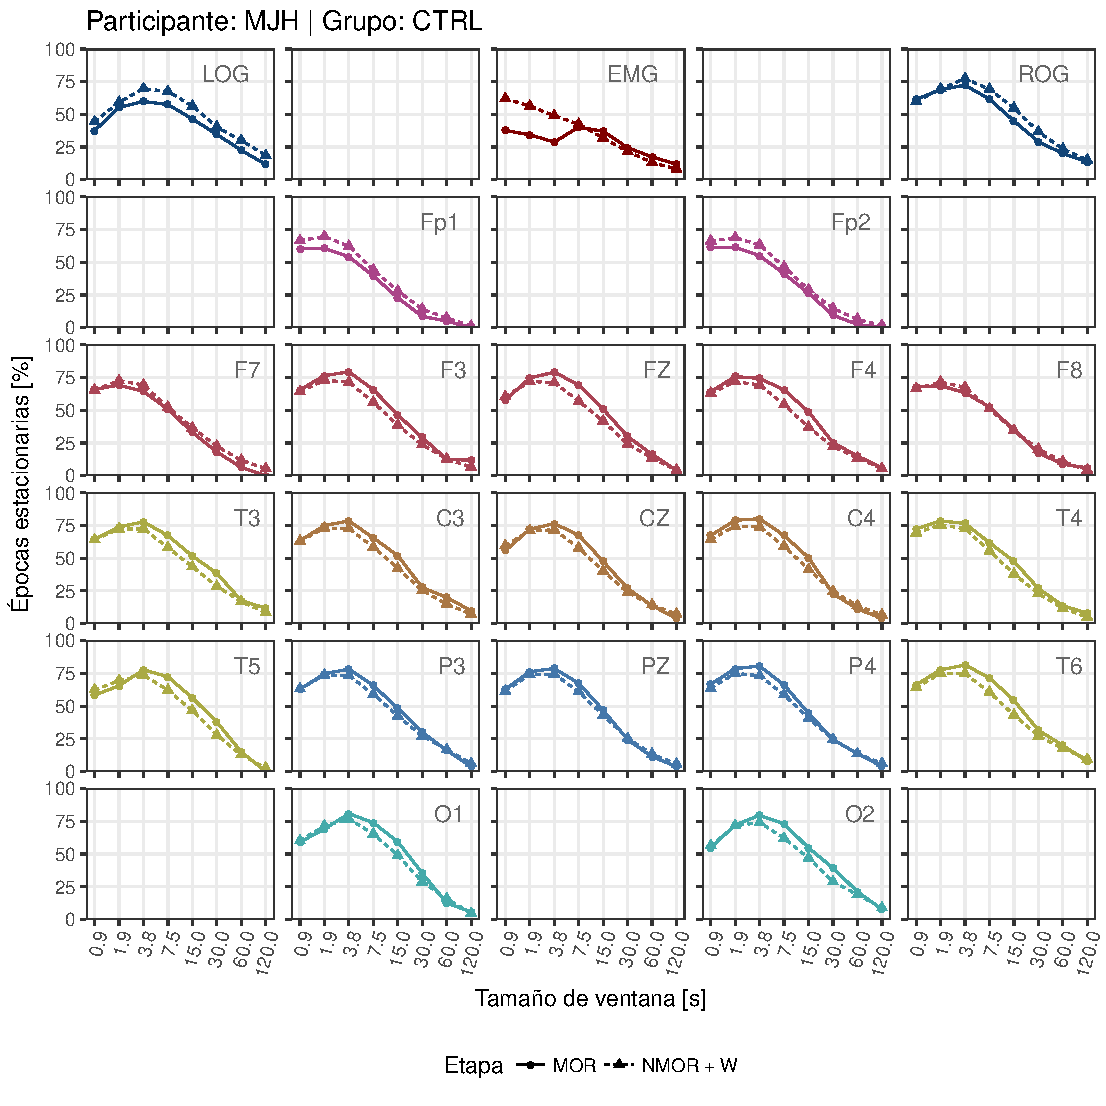
\includegraphics[width=\linewidth]{./scripts_graf_res/MJNNVIGILOS_cabeza_epocas_v2.pdf}
\caption{Cambio en la proporción de épocas estacionarias respecto al tamaño de ventana usado, durante MOR y NMOR. El análisis se repite en todas las derivaciones consideradas; la posición y color de cada gráfico se corresponden a aquellos de la figura \ref{img:estampa}. Sea abrevia W = vigilia, recordando que la cantidad tiempo de los registros clasificada como vigilia es negligible.}
 
\end{figure}

\begin{figure}
\centering
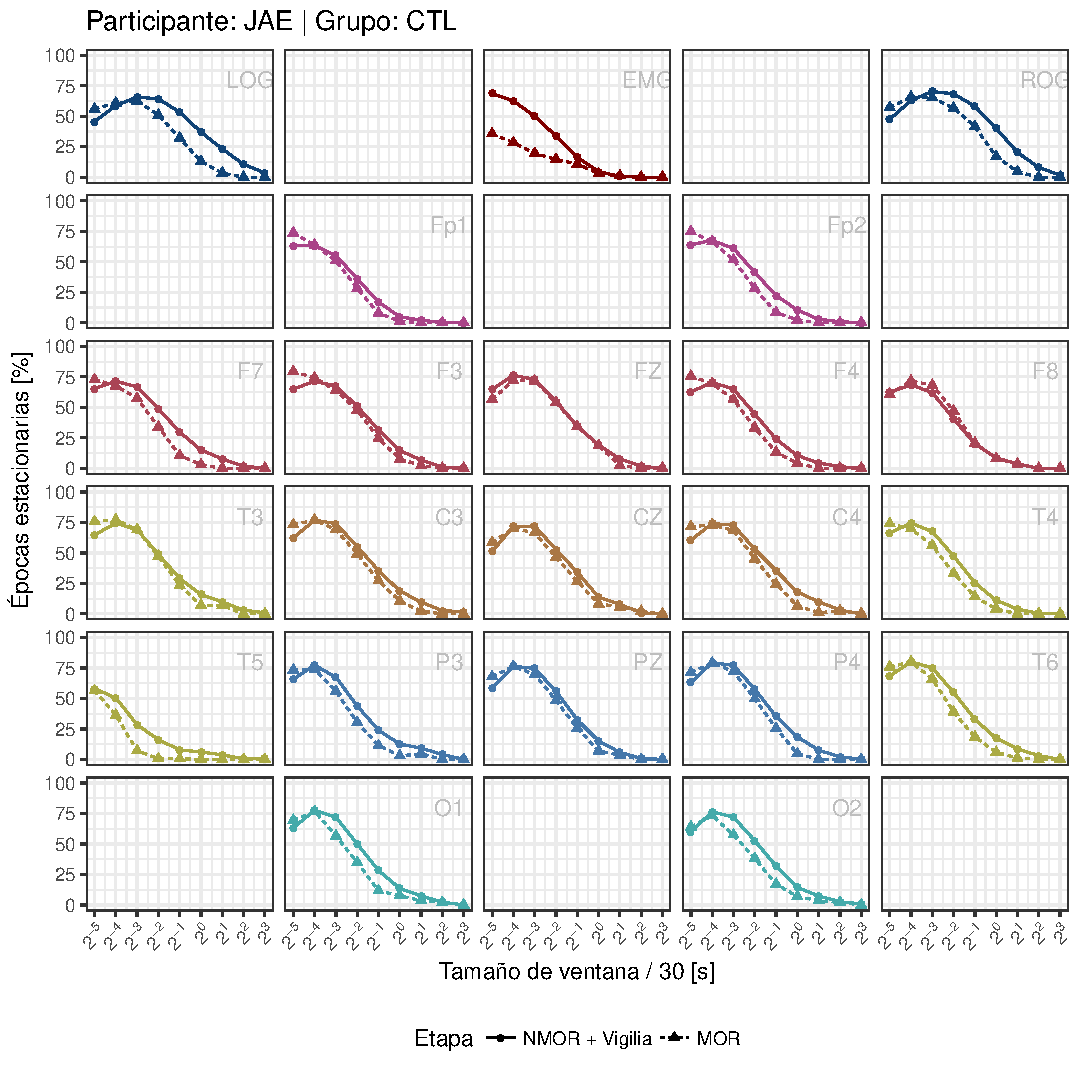
\includegraphics[width=\linewidth]{./scripts_graf_res/JANASUE_cabeza_epocas_v2.pdf}
\caption{Cambio en la proporción de épocas estacionarias respecto al tamaño de ventana usado, durante MOR y NMOR. El análisis se repite en todas las derivaciones consideradas; la posición y color de cada gráfico se corresponden a aquellos de la figura \ref{img:estampa}. Sea abrevia W = vigilia, recordando que la cantidad tiempo de los registros clasificada como vigilia es negligible.}
 
\end{figure}

\begin{figure}
\centering
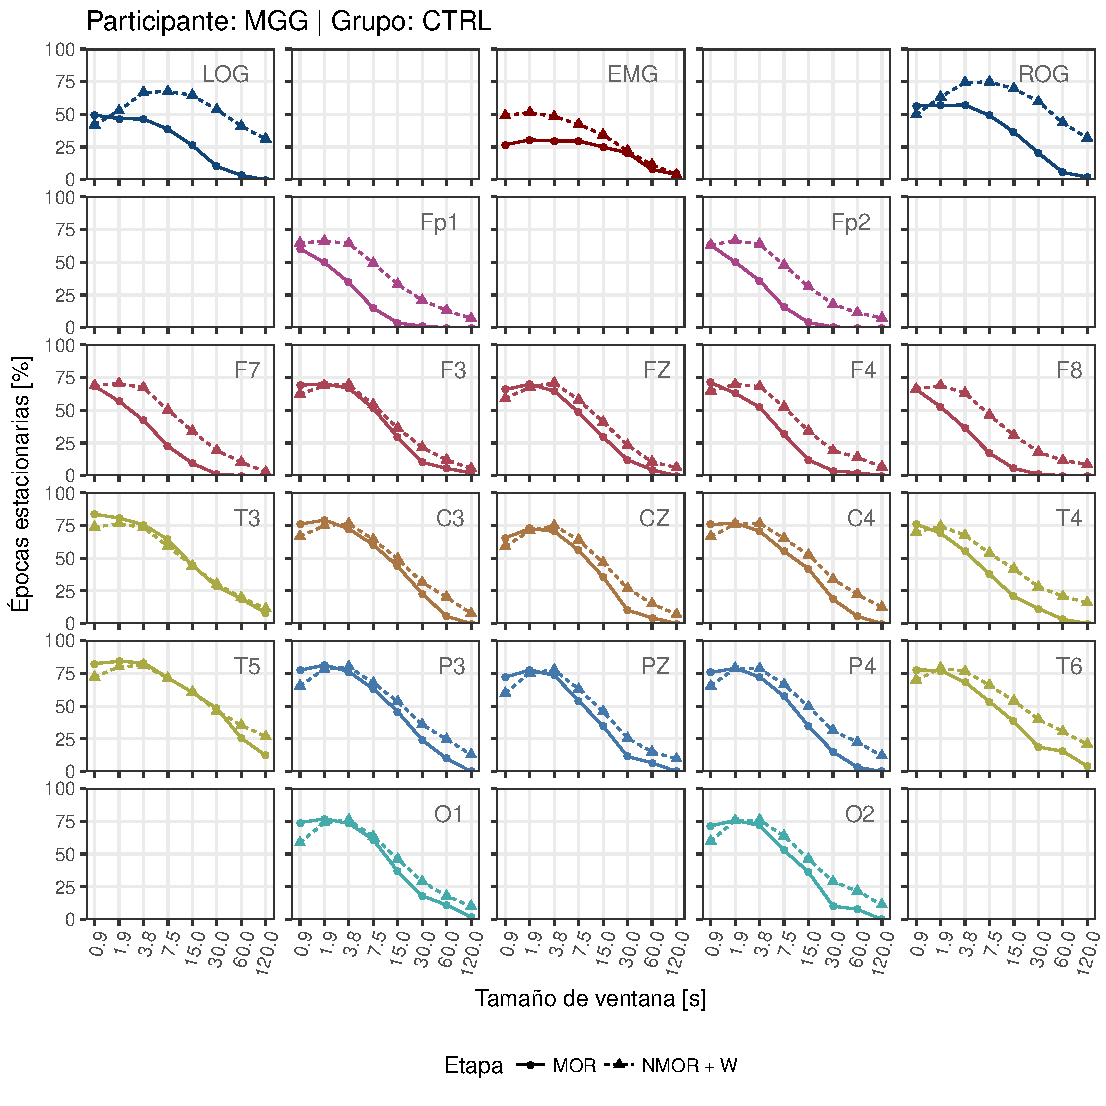
\includegraphics[width=\linewidth]{./scripts_graf_res/MGNA5SUE_cabeza_epocas_v2.pdf}
\caption{Cambio en la proporción de épocas estacionarias respecto al tamaño de ventana usado, durante MOR y NMOR. El análisis se repite en todas las derivaciones consideradas; la posición y color de cada gráfico se corresponden a aquellos de la figura \ref{img:estampa}. Sea abrevia W = vigilia, recordando que la cantidad tiempo de los registros clasificada como vigilia es negligible.}
 
\end{figure}

\begin{figure}
\centering
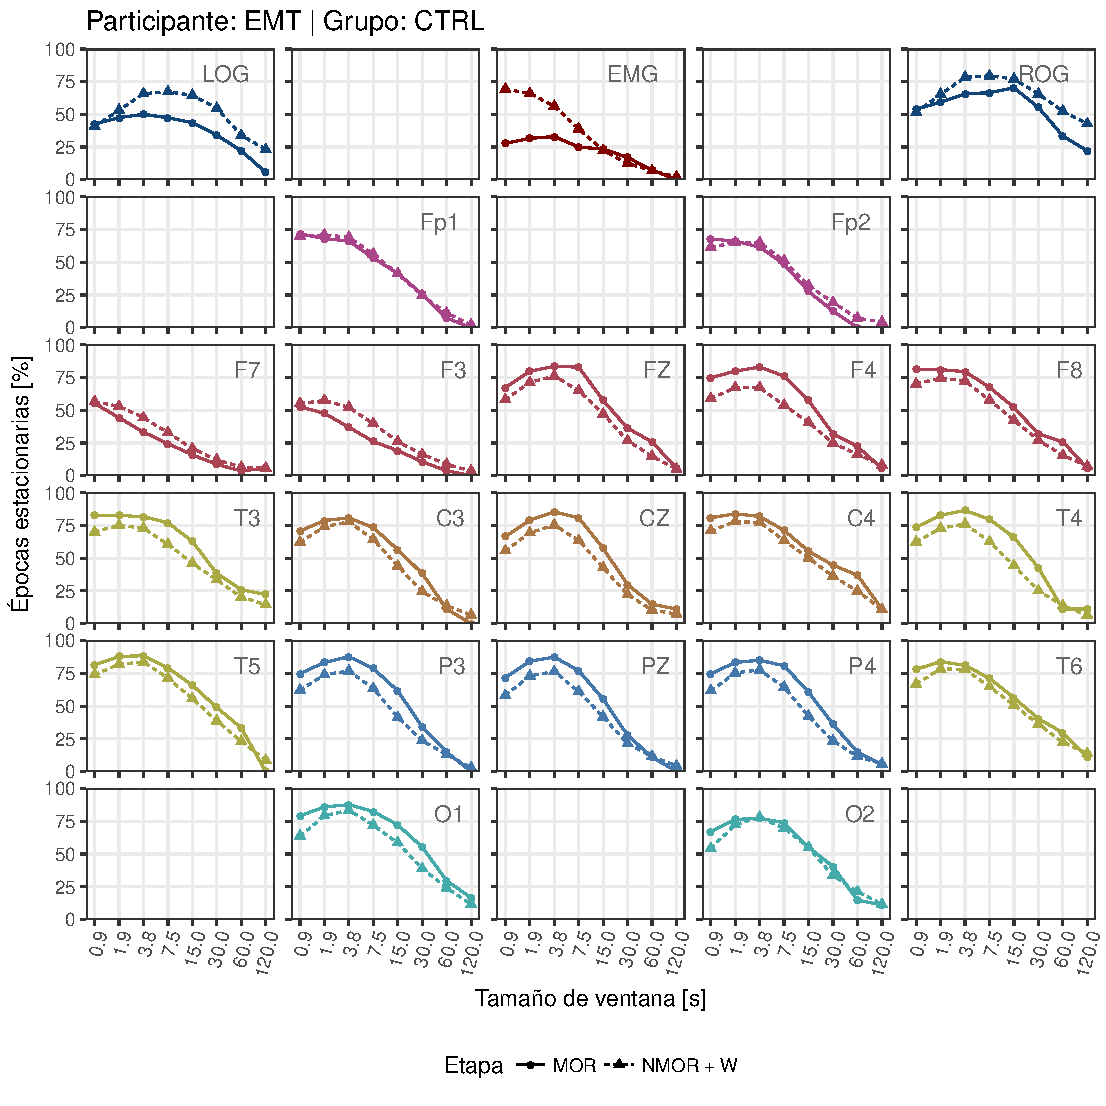
\includegraphics[width=\linewidth]{./scripts_graf_res/EMNNS_cabeza_epocas_v2.pdf}
\caption{Cambio en la proporción de épocas estacionarias respecto al tamaño de ventana usado, durante MOR y NMOR. El análisis se repite en todas las derivaciones consideradas; la posición y color de cada gráfico se corresponden a aquellos de la figura \ref{img:estampa}. Sea abrevia W = vigilia, recordando que la cantidad tiempo de los registros clasificada como vigilia es negligible.}
 
\end{figure}

\begin{figure}
\centering
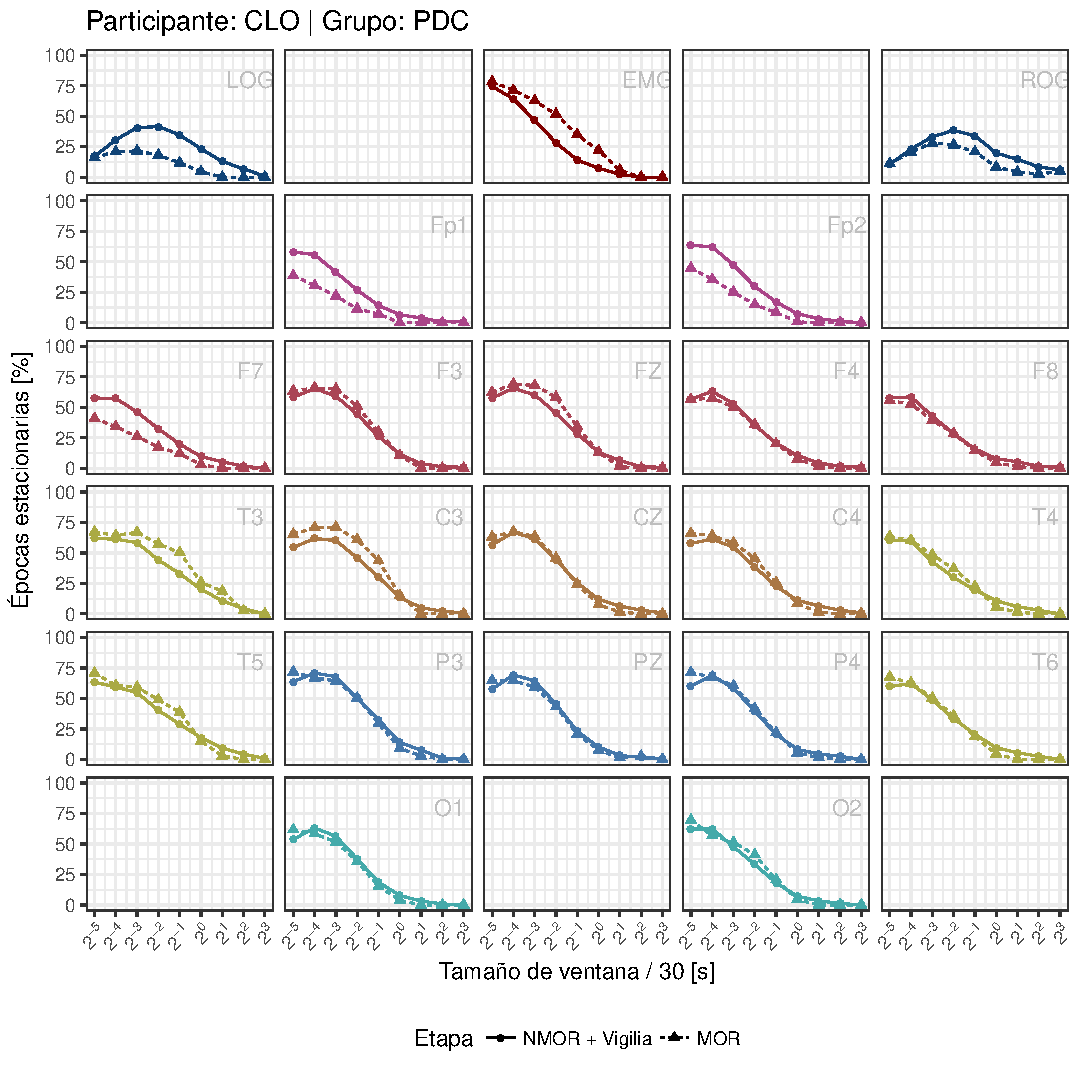
\includegraphics[width=\linewidth]{./scripts_graf_res/CLMN10SUE_cabeza_epocas_v2.pdf}
\caption{Cambio en la proporción de épocas estacionarias respecto al tamaño de ventana usado, durante MOR y NMOR. El análisis se repite en todas las derivaciones consideradas; la posición y color de cada gráfico se corresponden a aquellos de la figura \ref{img:estampa}. Sea abrevia W = vigilia, recordando que la cantidad tiempo de los registros clasificada como vigilia es negligible.}
 
\end{figure}

\begin{figure}
\centering
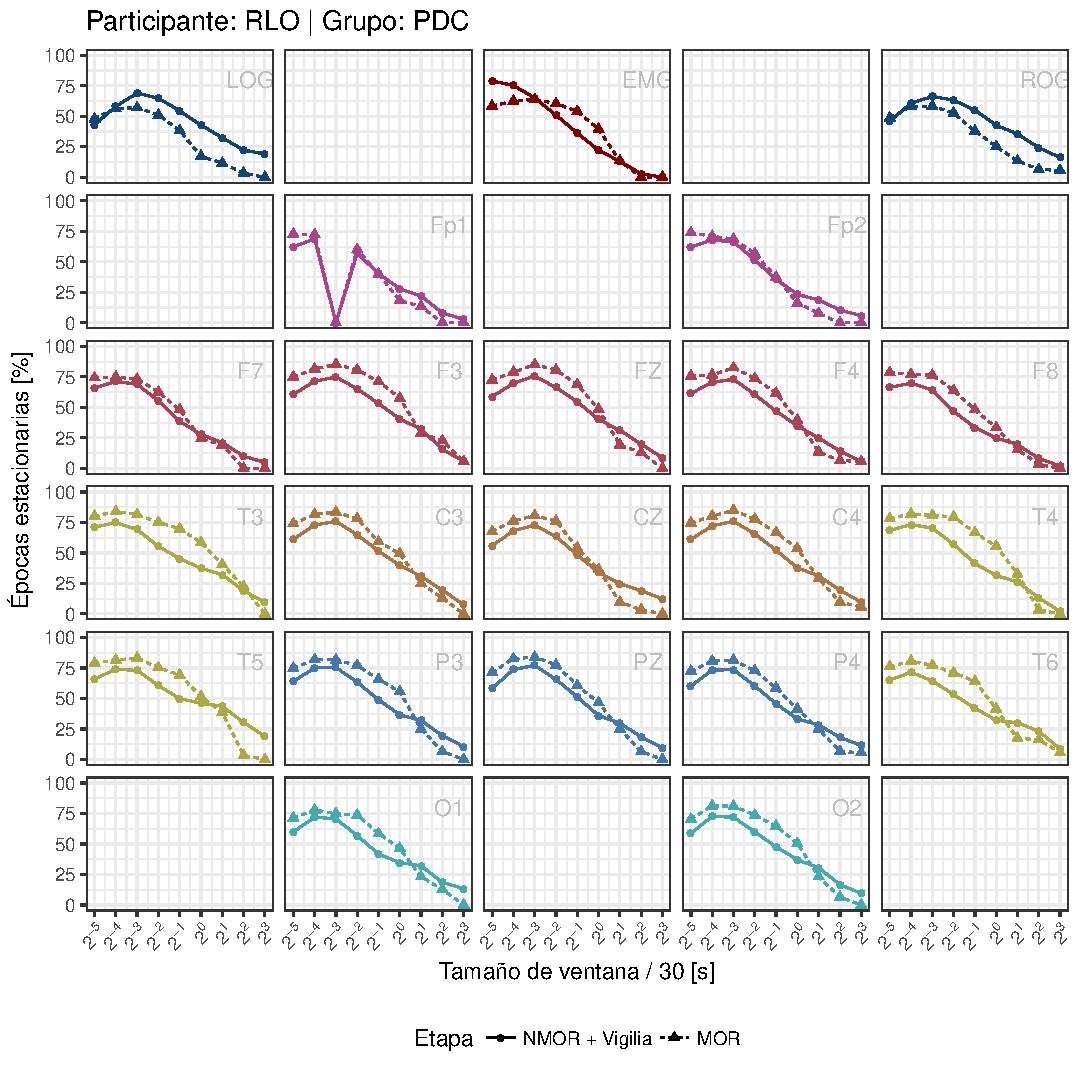
\includegraphics[width=\linewidth]{./scripts_graf_res/RLMN10SUE_cabeza_epocas_v2.pdf}
\caption{Cambio en la proporción de épocas estacionarias respecto al tamaño de ventana usado, durante MOR y NMOR. El análisis se repite en todas las derivaciones consideradas; la posición y color de cada gráfico se corresponden a aquellos de la figura \ref{img:estampa}. Sea abrevia W = vigilia, recordando que la cantidad tiempo de los registros clasificada como vigilia es negligible.}
 
\end{figure}

\begin{figure}
\centering
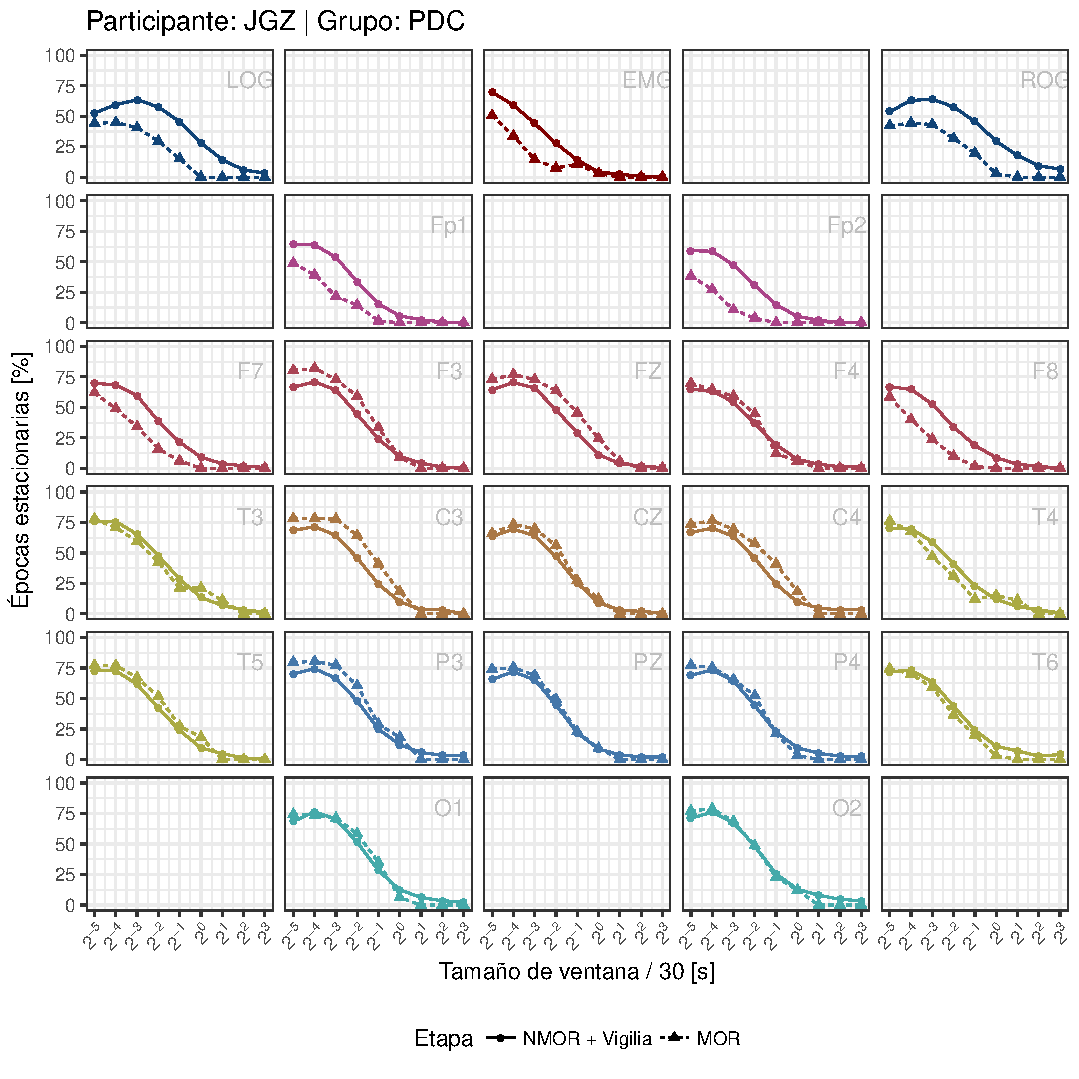
\includegraphics[width=\linewidth]{./scripts_graf_res/JGMN6SUE_cabeza_epocas_v2.pdf}
\caption{Cambio en la proporción de épocas estacionarias respecto al tamaño de ventana usado, durante MOR y NMOR. El análisis se repite en todas las derivaciones consideradas; la posición y color de cada gráfico se corresponden a aquellos de la figura \ref{img:estampa}. Sea abrevia W = vigilia, recordando que la cantidad tiempo de los registros clasificada como vigilia es negligible.}
 
\end{figure}

\begin{figure}
\centering
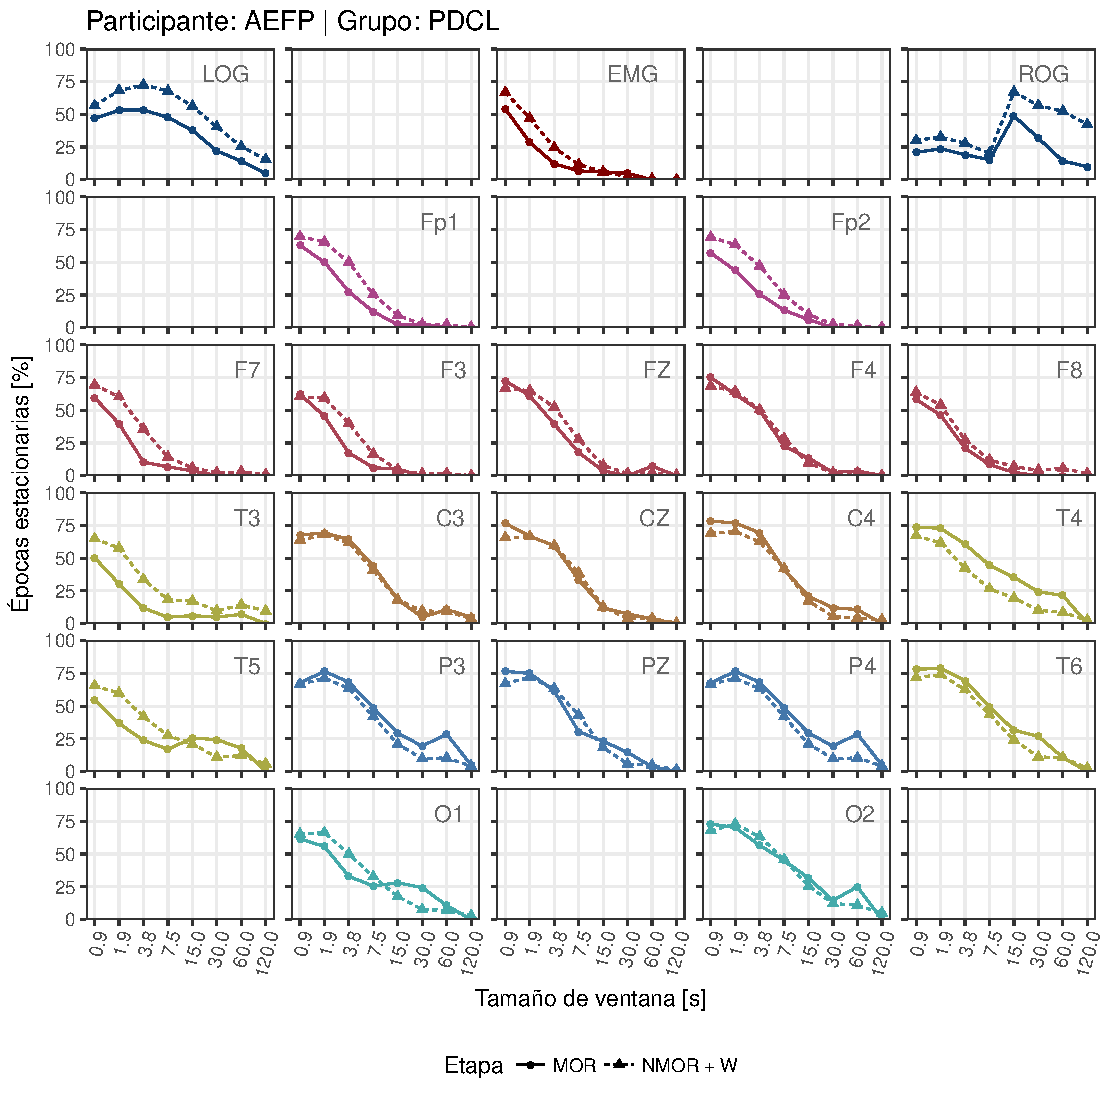
\includegraphics[width=\linewidth]{./scripts_graf_res/AEFP430714SUE_cabeza_epocas_v2.pdf}
\caption{Cambio en la proporción de épocas estacionarias respecto al tamaño de ventana usado, durante MOR y NMOR. El análisis se repite en todas las derivaciones consideradas; la posición y color de cada gráfico se corresponden a aquellos de la figura \ref{img:estampa}. Sea abrevia W = vigilia, recordando que la cantidad tiempo de los registros clasificada como vigilia es negligible.}
 
\end{figure}

\begin{figure}
\centering
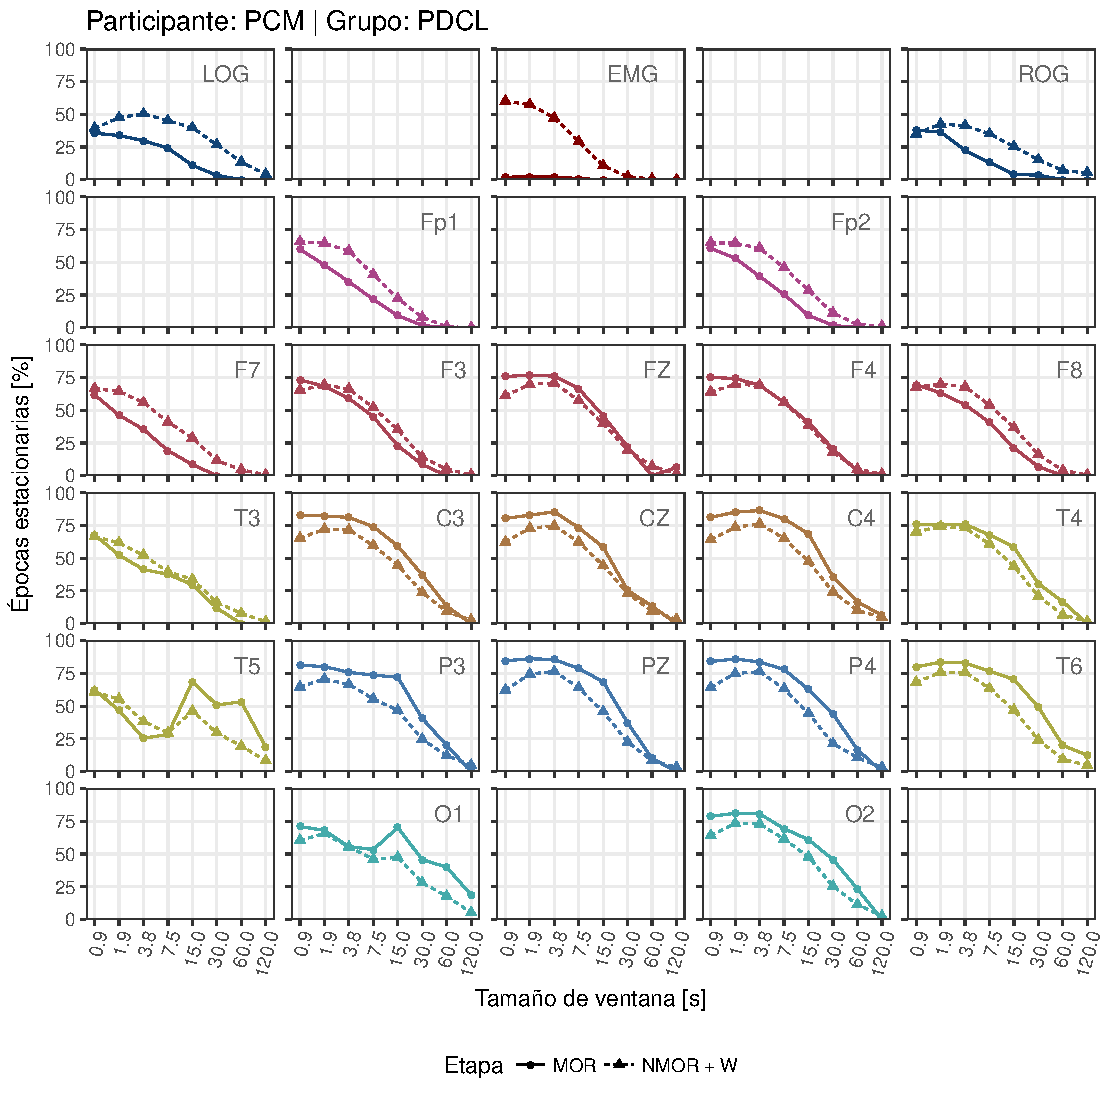
\includegraphics[width=\linewidth]{./scripts_graf_res/PCM90SUE_cabeza_epocas_v2.pdf}
\caption{Cambio en la proporción de épocas estacionarias respecto al tamaño de ventana usado, durante MOR y NMOR. El análisis se repite en todas las derivaciones consideradas; la posición y color de cada gráfico se corresponden a aquellos de la figura \ref{img:estampa}. Sea abrevia W = vigilia, recordando que la cantidad tiempo de los registros clasificada como vigilia es negligible.}
 
\end{figure}

%%%%%%%%%%%%%%%%%%%%%%%%%%%%%%%%%%%%%%%%%%%%%%%%%%%%%%%%%%%%%%%%%%%%%%%%%%%%%%%%%%%%%%%%%%%%%%%%%%%
%%%%%%%%%%%%%%%%%%%%%%%%%%%%%%%%%%%%%%%%%%%%%%%%%%%%%%%%%%%%%%%%%%%%%%%%%%%%%%%%%%%%%%%%%%%%%%%%%%%

\begin{figure}
\centering
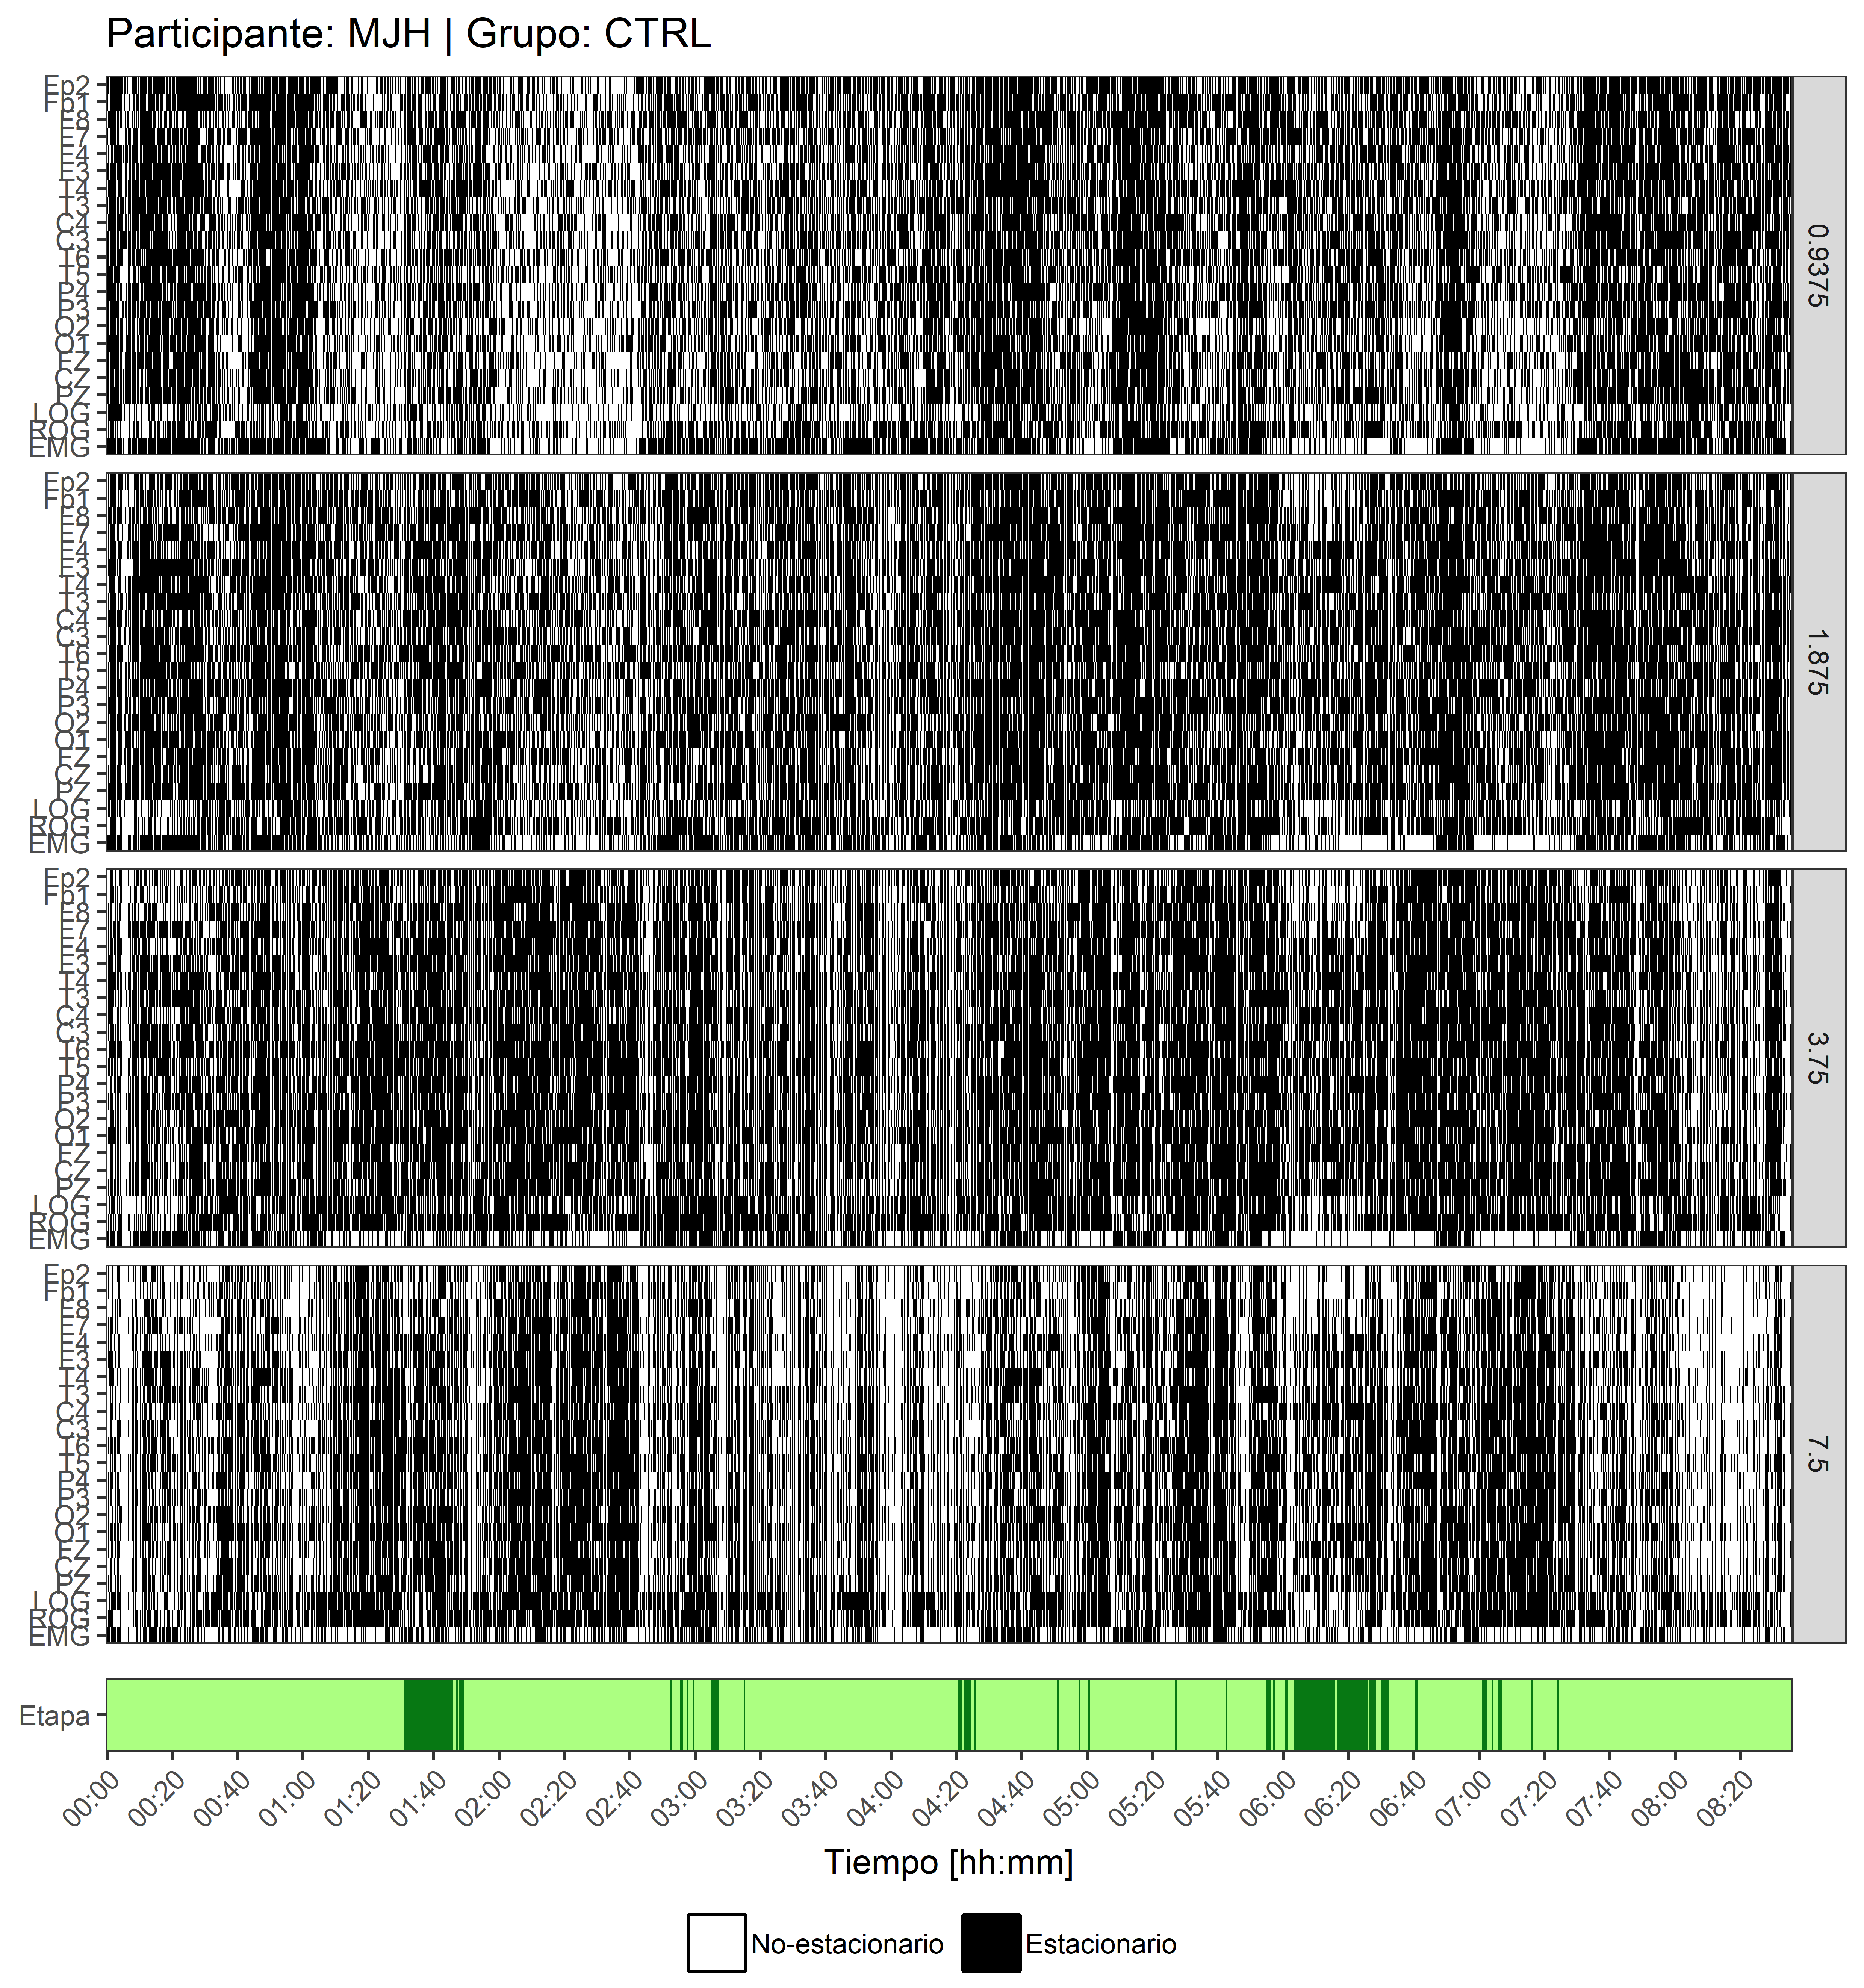
\includegraphics[width=\linewidth]
{./scripts_graf_res/MJH_patrones_1.png}
\caption[Distribución en el tiempo de las ventanas clasificadas como estacionarias, considerando diferentes tamaños de ventana]{Distribución en el tiempo de las ventanas clasificadas como estacionarias, considerando diferentes tamaños de ventana. 
Cada ventana fue representada en una cuadrícula según su derivación (margen izquierdo) y momento (margen inferior) de procedencia; posteriormente fue \textit{coloreada} según su clasificación como estacionaria.
Dado que la clasificación de estacionariedad se repitió usando diversos tamaños de ventana, éstos se indican en el margen derecho.
En la parte inferior se representan las mismas épocas en su clasificación según etapa de sueño.}
\end{figure}
\begin{figure}
\centering
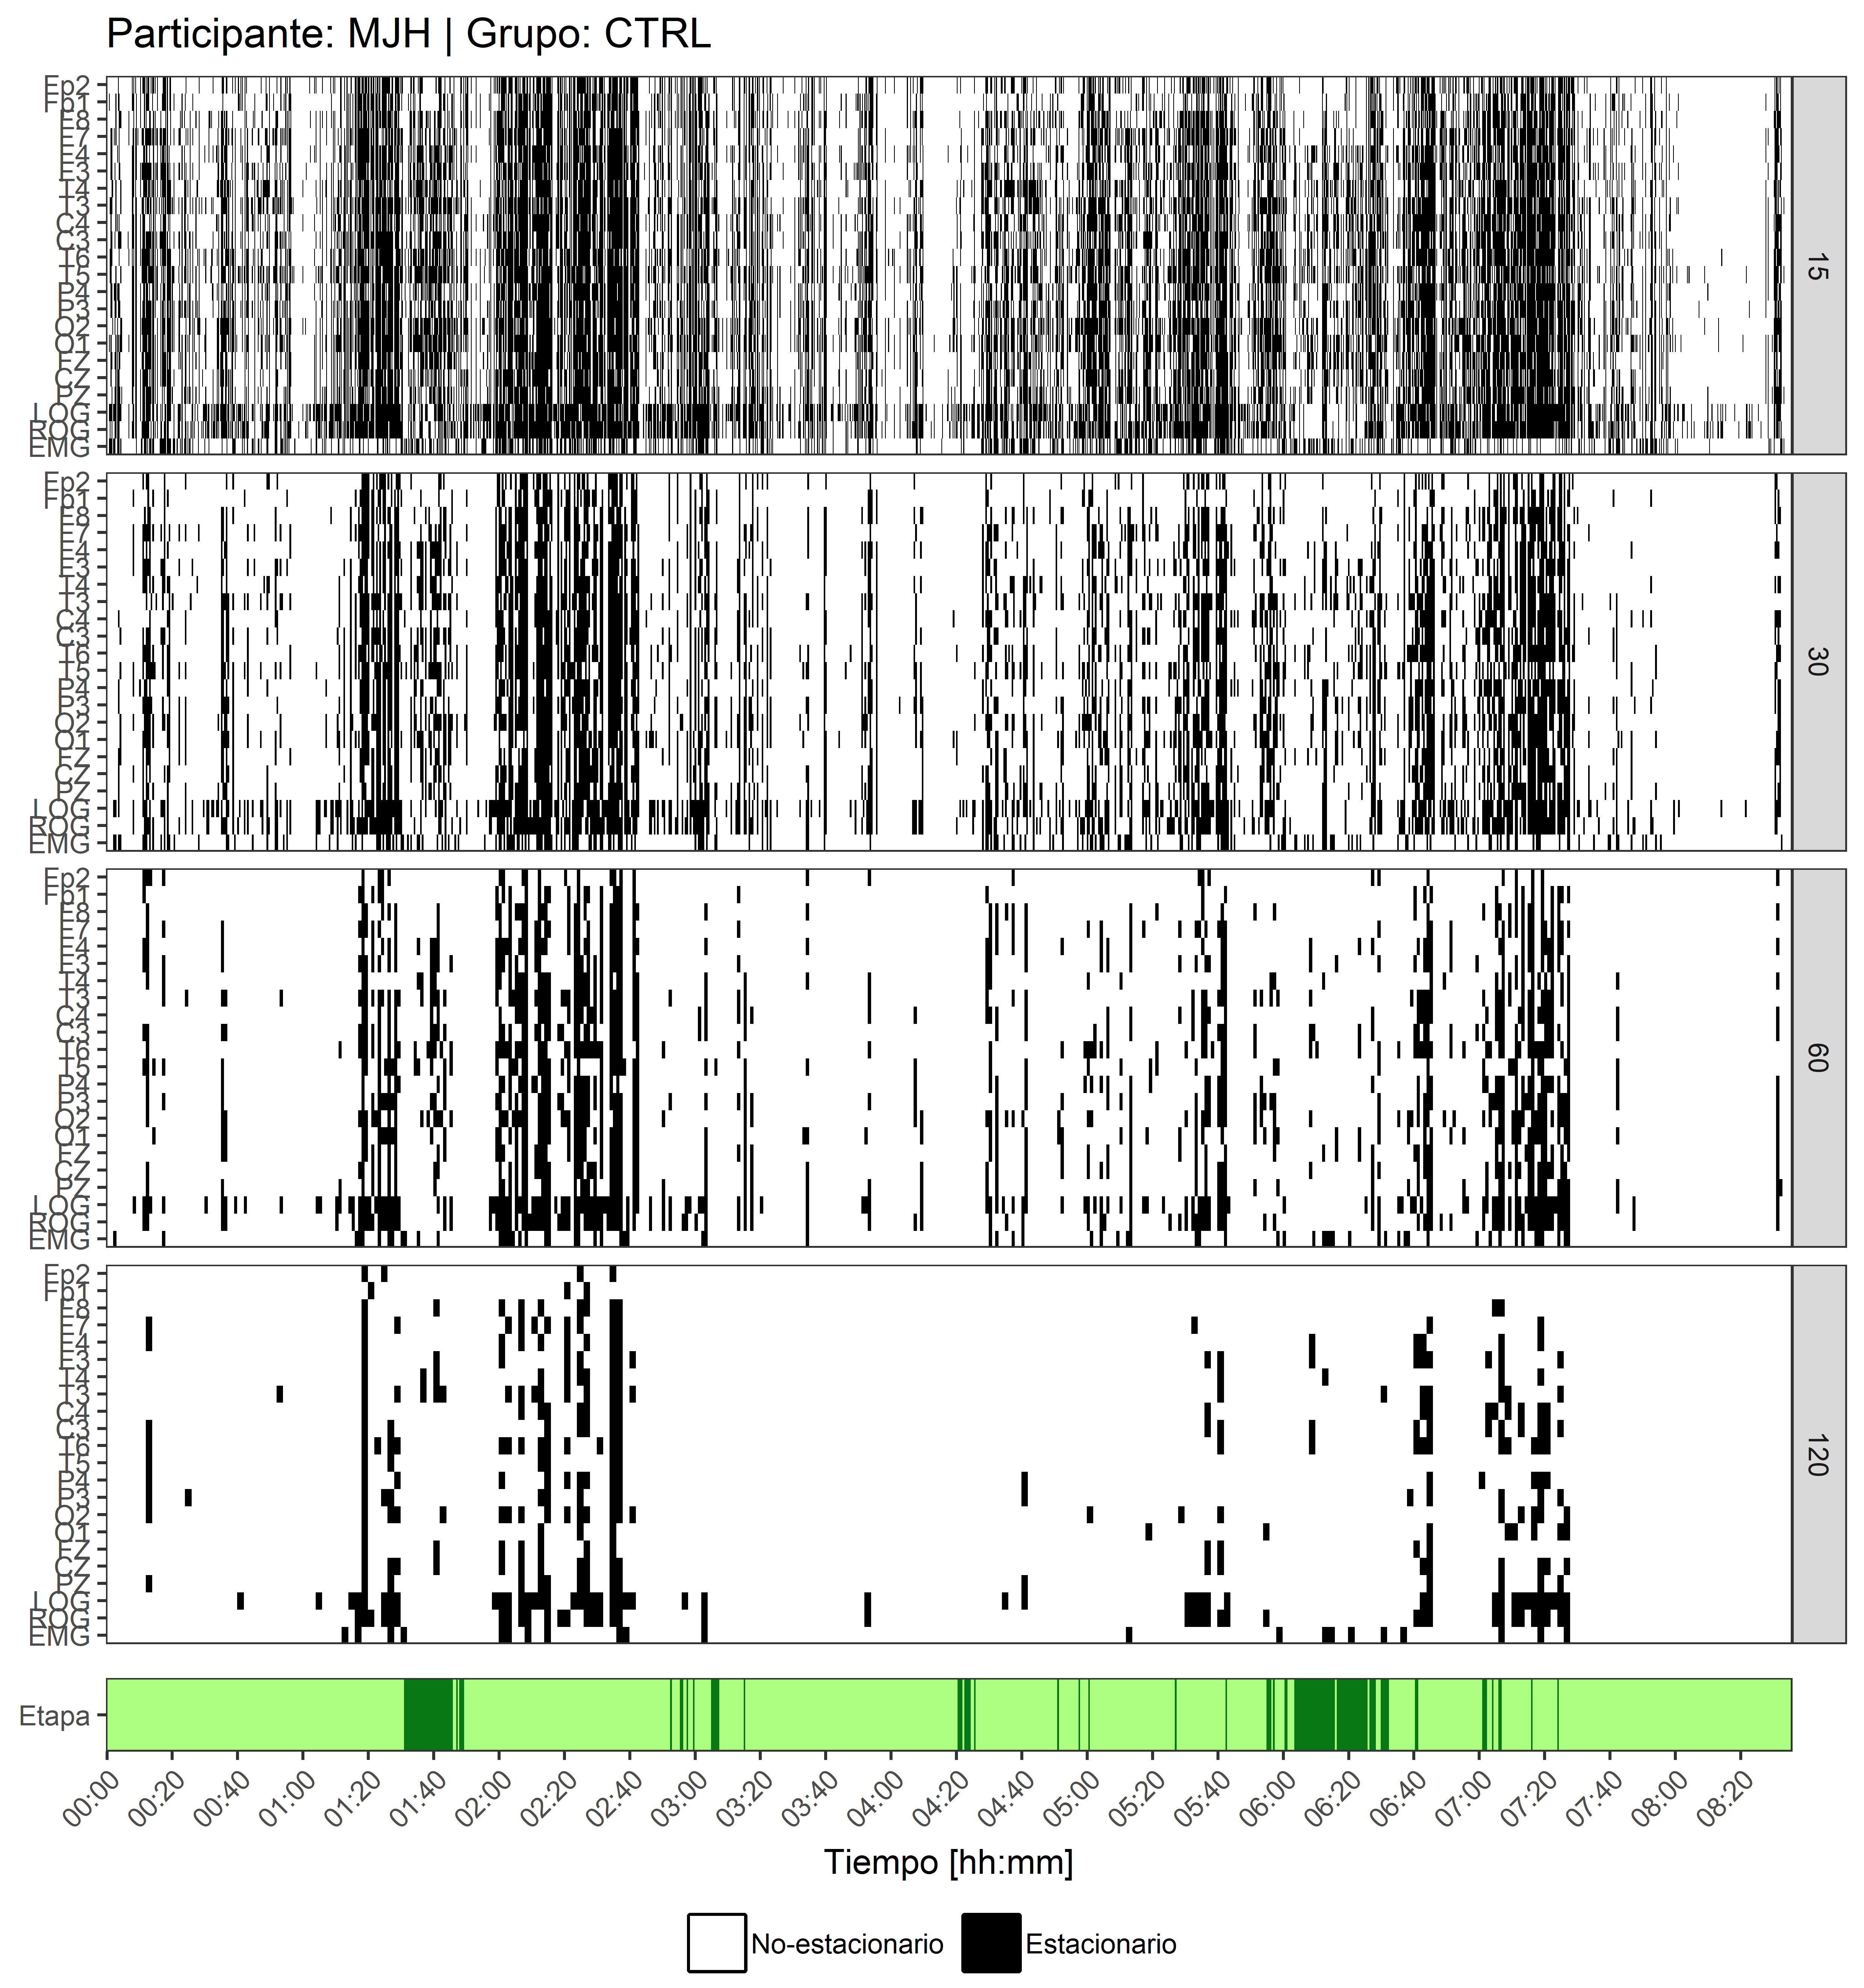
\includegraphics[width=\linewidth]
{./scripts_graf_res/MJH_patrones_2.png}
\caption[Distribución en el tiempo de las ventanas clasificadas como estacionarias, considerando diferentes tamaños de ventana]{Distribución en el tiempo de las ventanas clasificadas como estacionarias, considerando diferentes tamaños de ventana. 
Cada ventana fue representada en una cuadrícula según su derivación (margen izquierdo) y momento (margen inferior) de procedencia; posteriormente fue \textit{coloreada} según su clasificación como estacionaria.
Dado que la clasificación de estacionariedad se repitió usando diversos tamaños de ventana, éstos se indican en el margen derecho.
En la parte inferior se representan las mismas épocas en su clasificación según etapa de sueño.}
\end{figure}


\begin{figure}
\centering
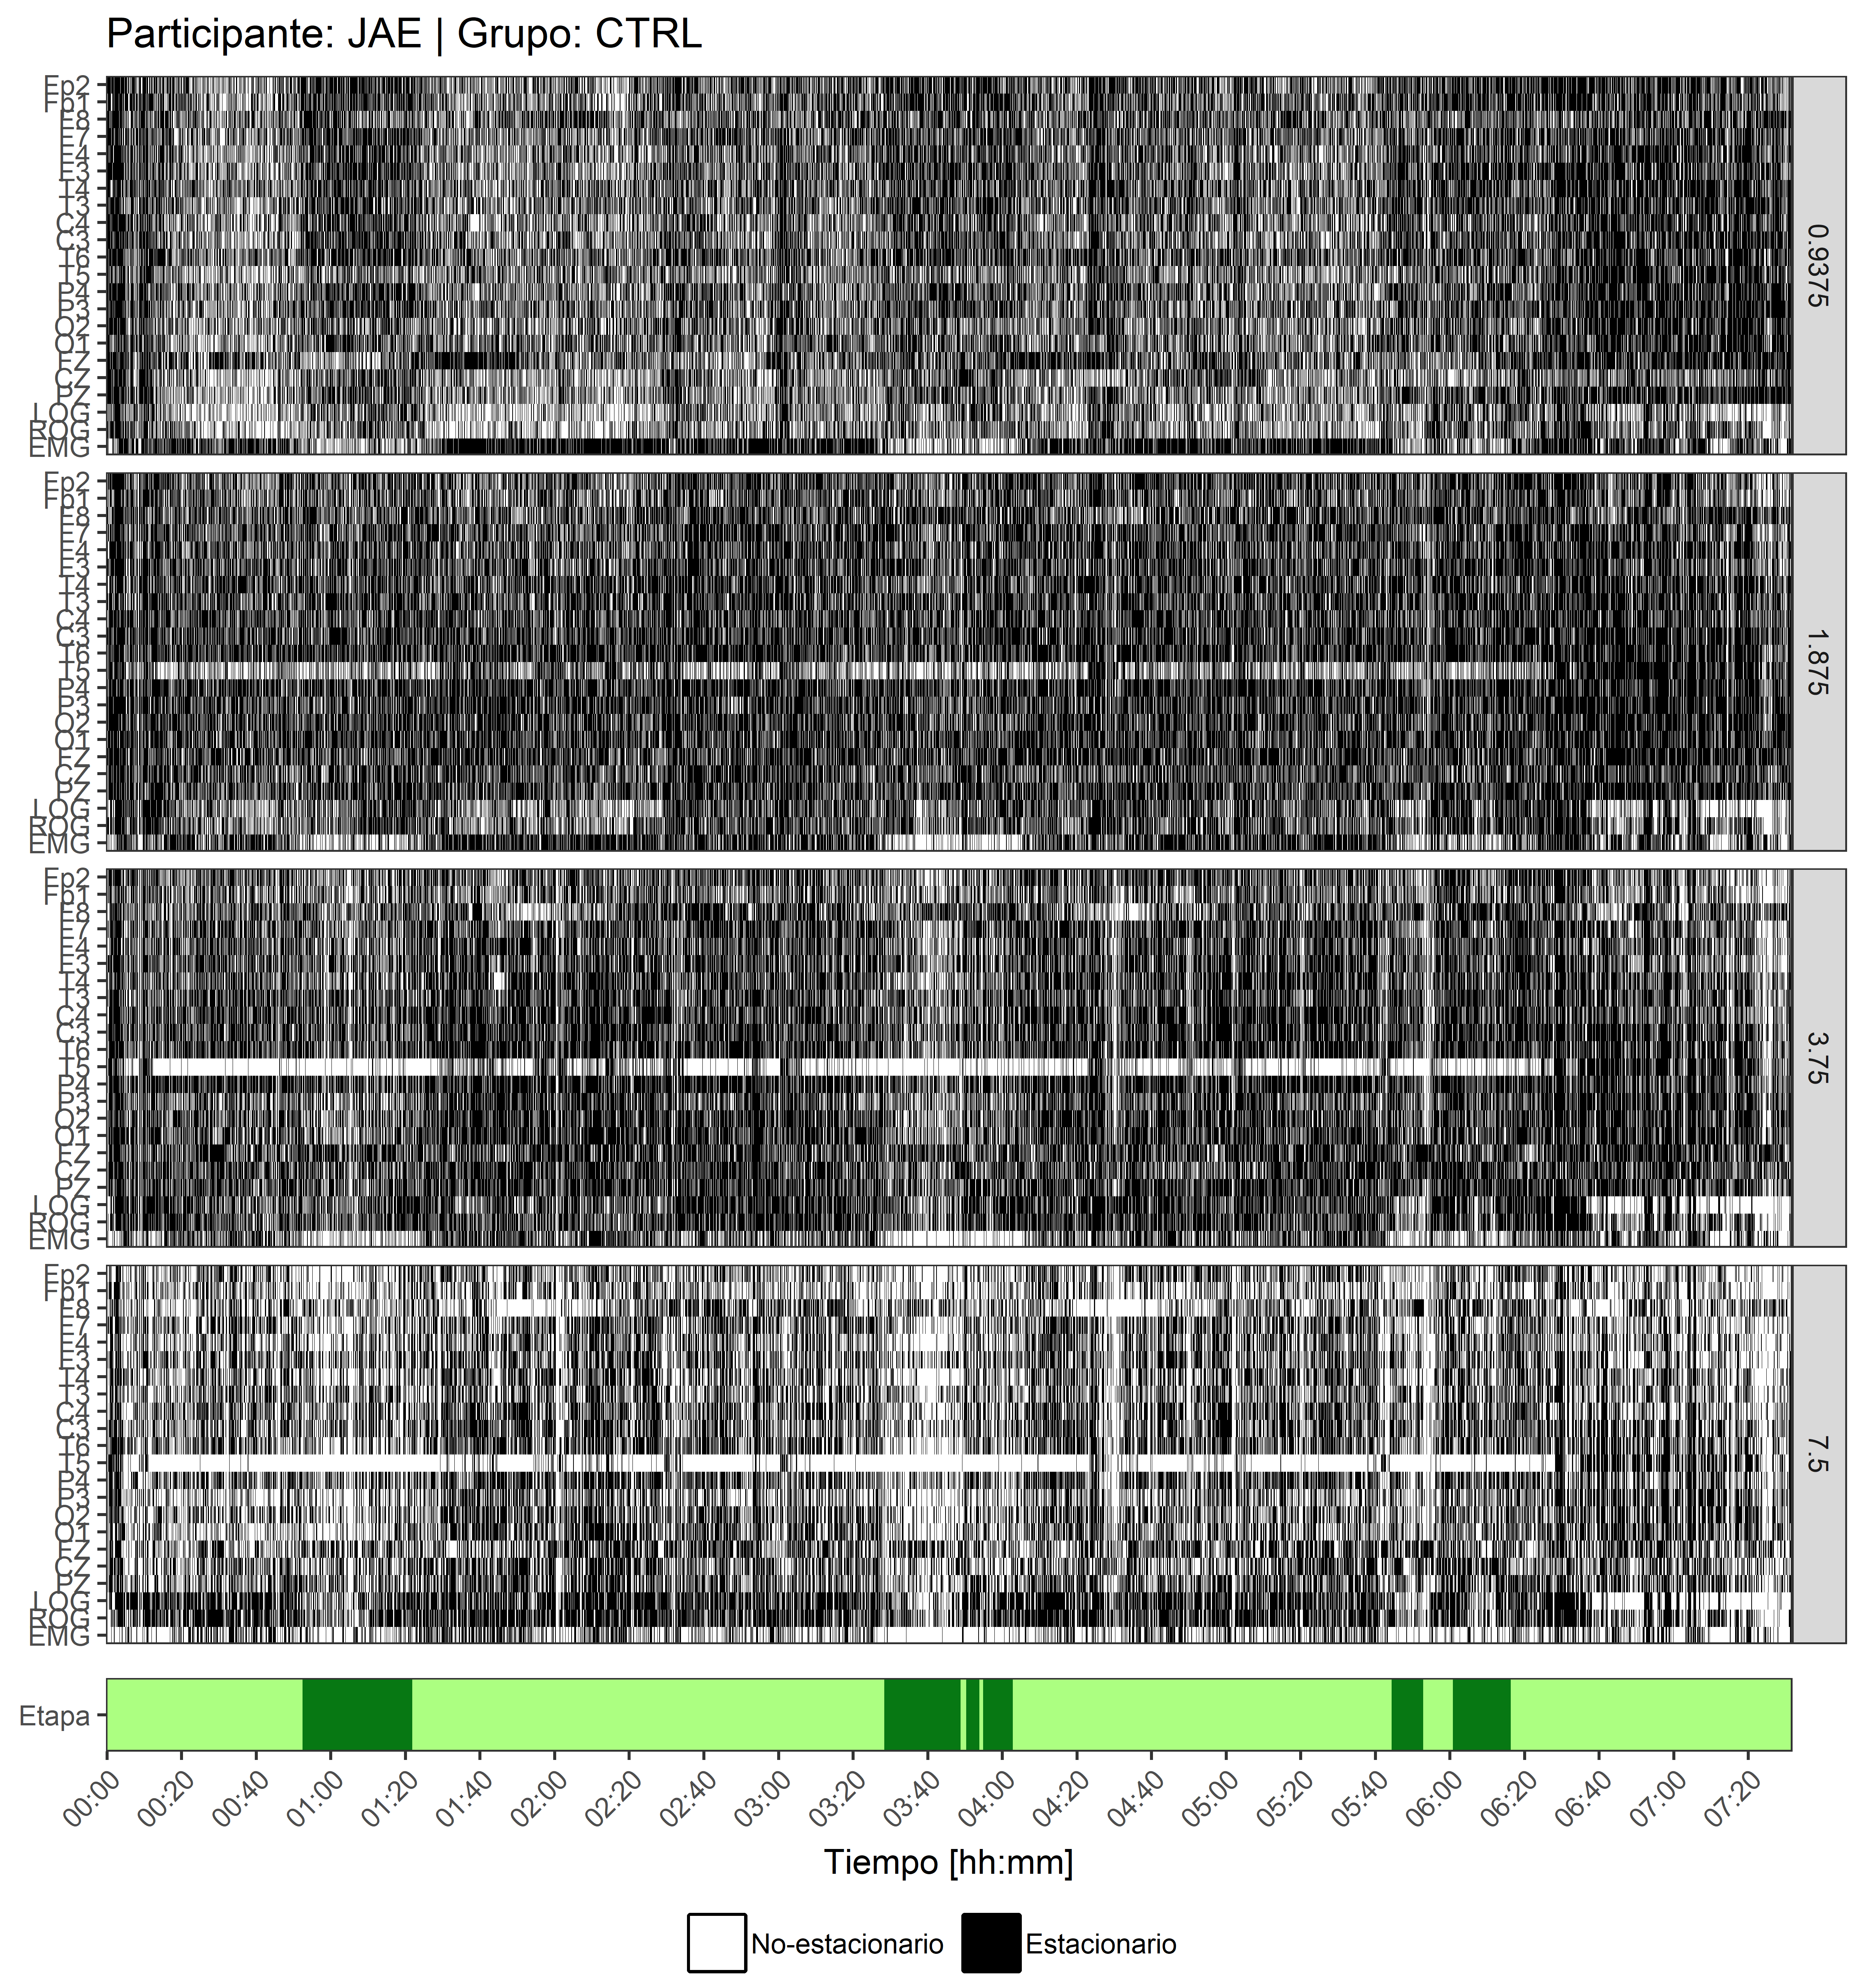
\includegraphics[width=\linewidth]
{./scripts_graf_res/JAE_patrones_1.png}
\caption[Distribución en el tiempo de las ventanas clasificadas como estacionarias, considerando diferentes tamaños de ventana]{Distribución en el tiempo de las ventanas clasificadas como estacionarias, considerando diferentes tamaños de ventana. 
Cada ventana fue representada en una cuadrícula según su derivación (margen izquierdo) y momento (margen inferior) de procedencia; posteriormente fue \textit{coloreada} según su clasificación como estacionaria.
Dado que la clasificación de estacionariedad se repitió usando diversos tamaños de ventana, éstos se indican en el margen derecho.
En la parte inferior se representan las mismas épocas en su clasificación según etapa de sueño.}
\end{figure}
\begin{figure}
\centering
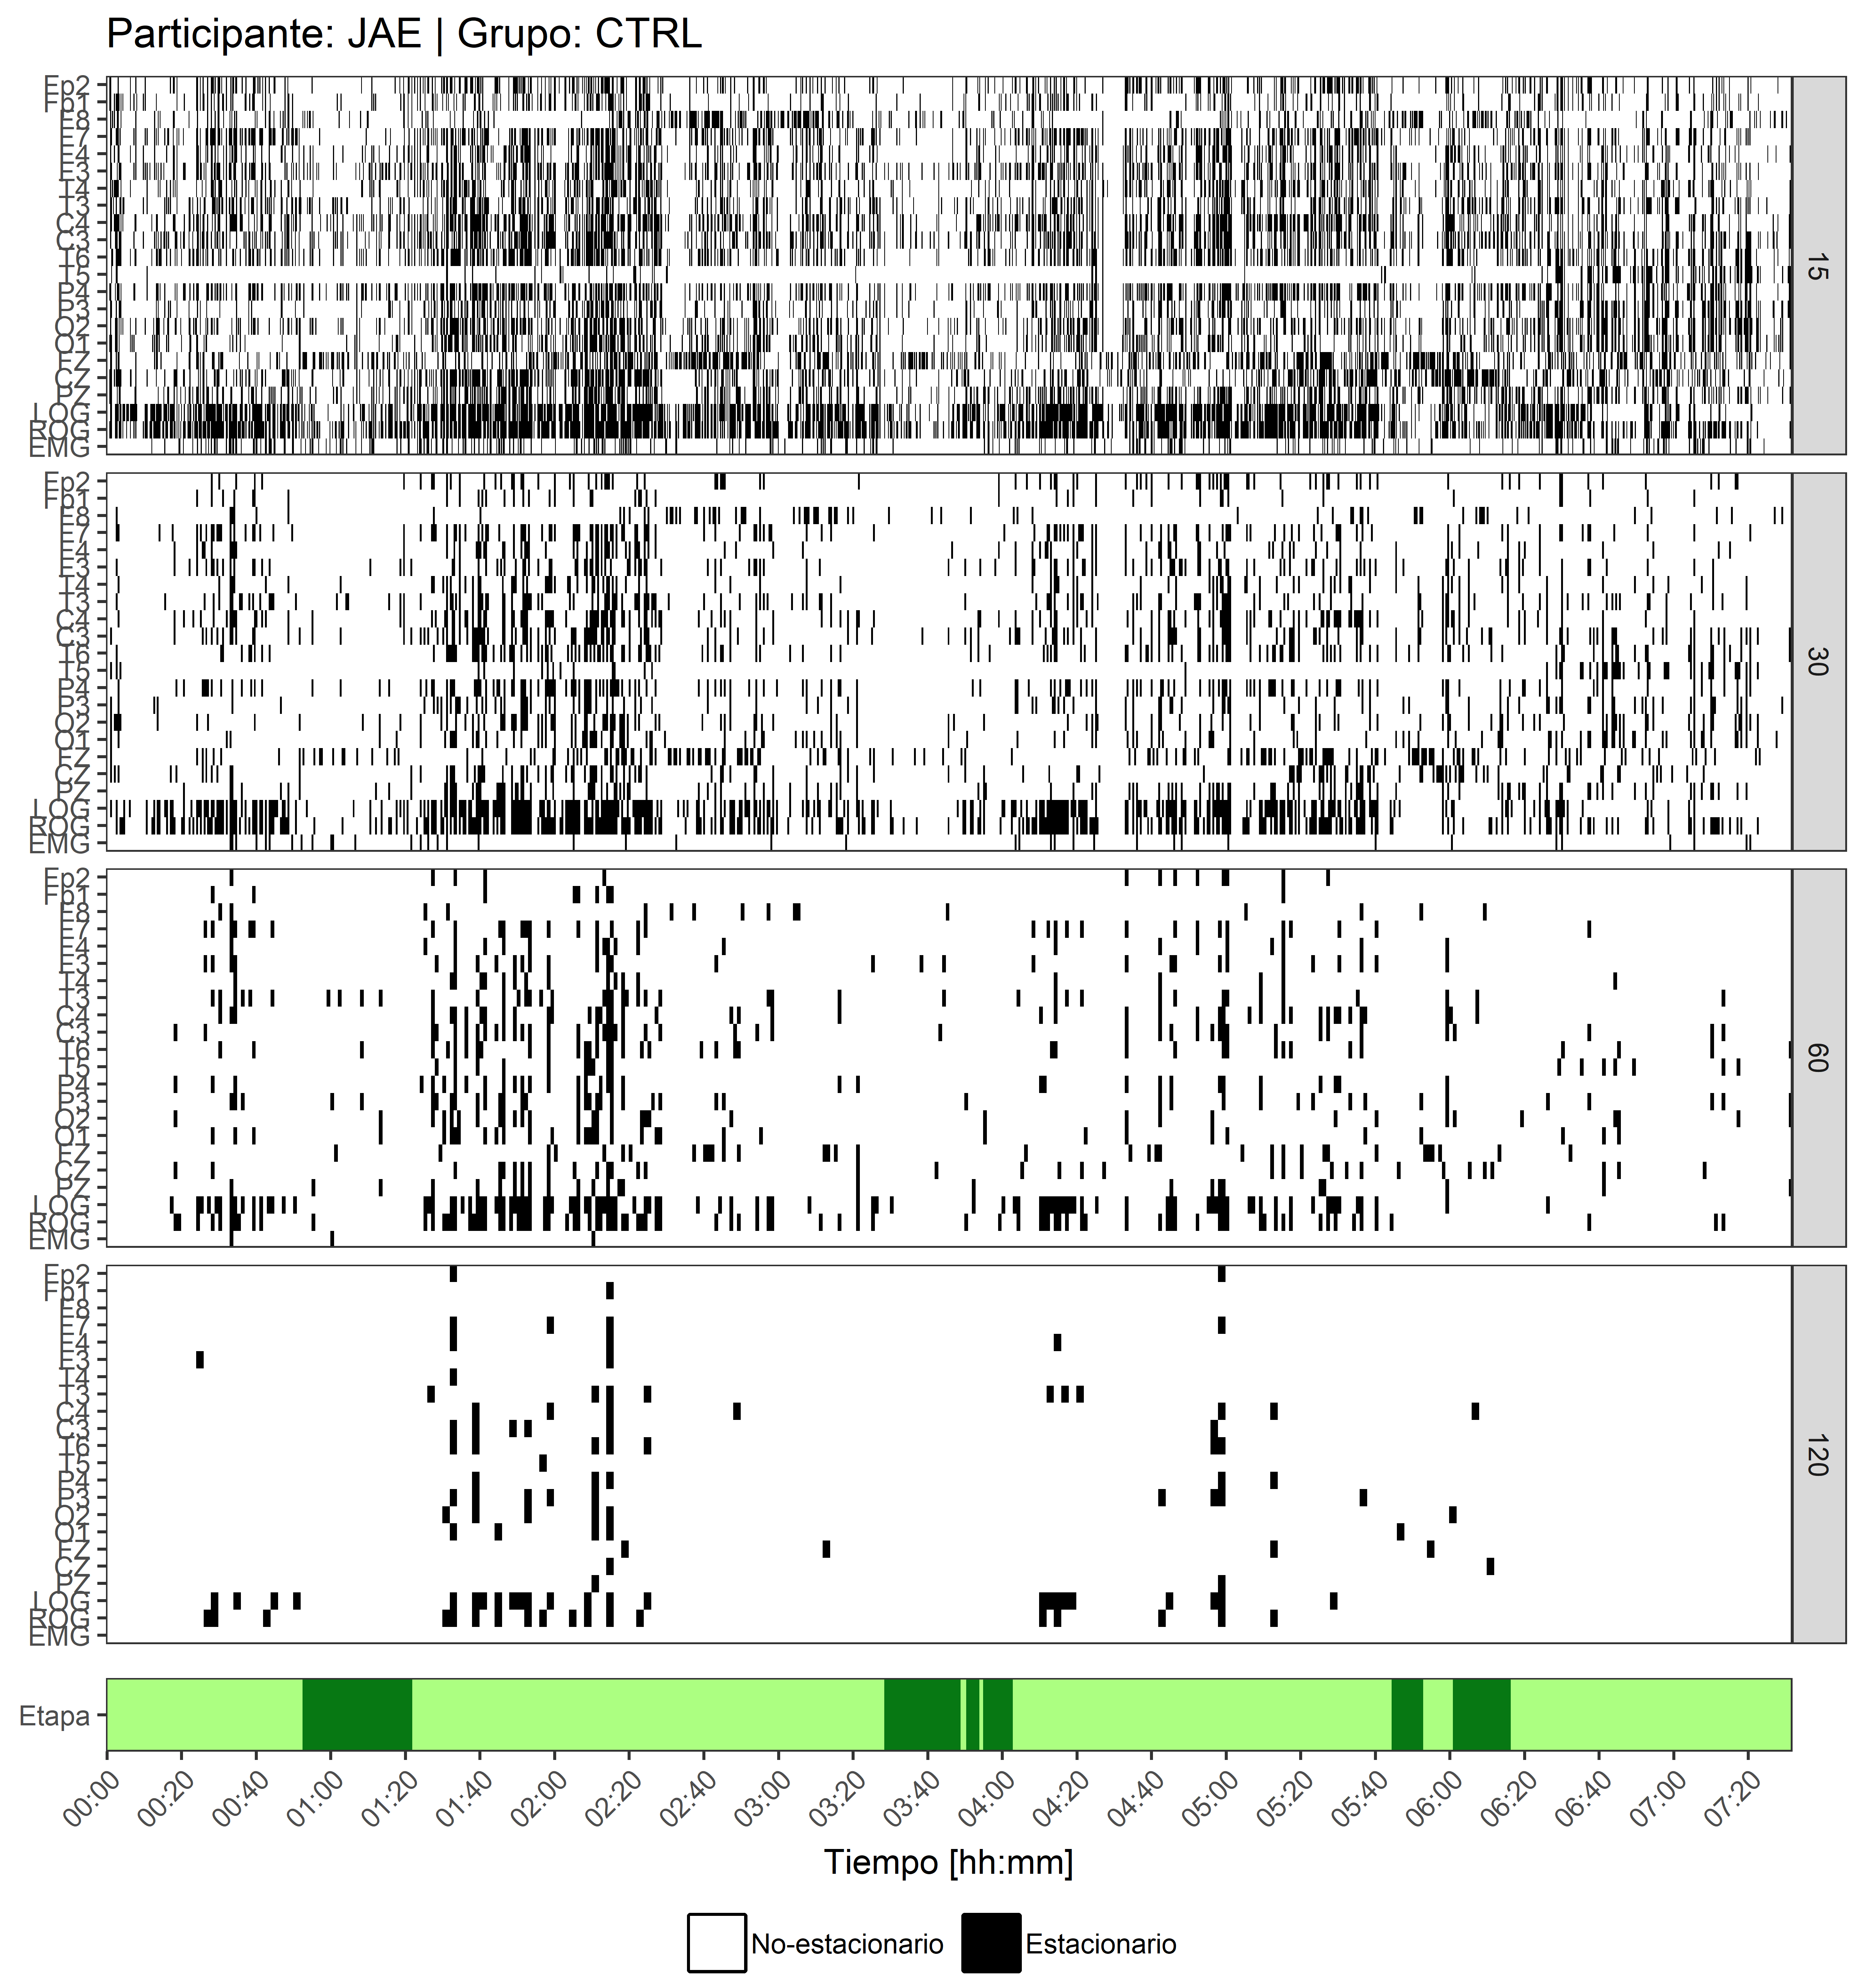
\includegraphics[width=\linewidth]
{./scripts_graf_res/JAE_patrones_2.png}
\caption[Distribución en el tiempo de las ventanas clasificadas como estacionarias, considerando diferentes tamaños de ventana]{Distribución en el tiempo de las ventanas clasificadas como estacionarias, considerando diferentes tamaños de ventana. 
Cada ventana fue representada en una cuadrícula según su derivación (margen izquierdo) y momento (margen inferior) de procedencia; posteriormente fue \textit{coloreada} según su clasificación como estacionaria.
Dado que la clasificación de estacionariedad se repitió usando diversos tamaños de ventana, éstos se indican en el margen derecho.
En la parte inferior se representan las mismas épocas en su clasificación según etapa de sueño.}
\end{figure}


\begin{figure}
\centering
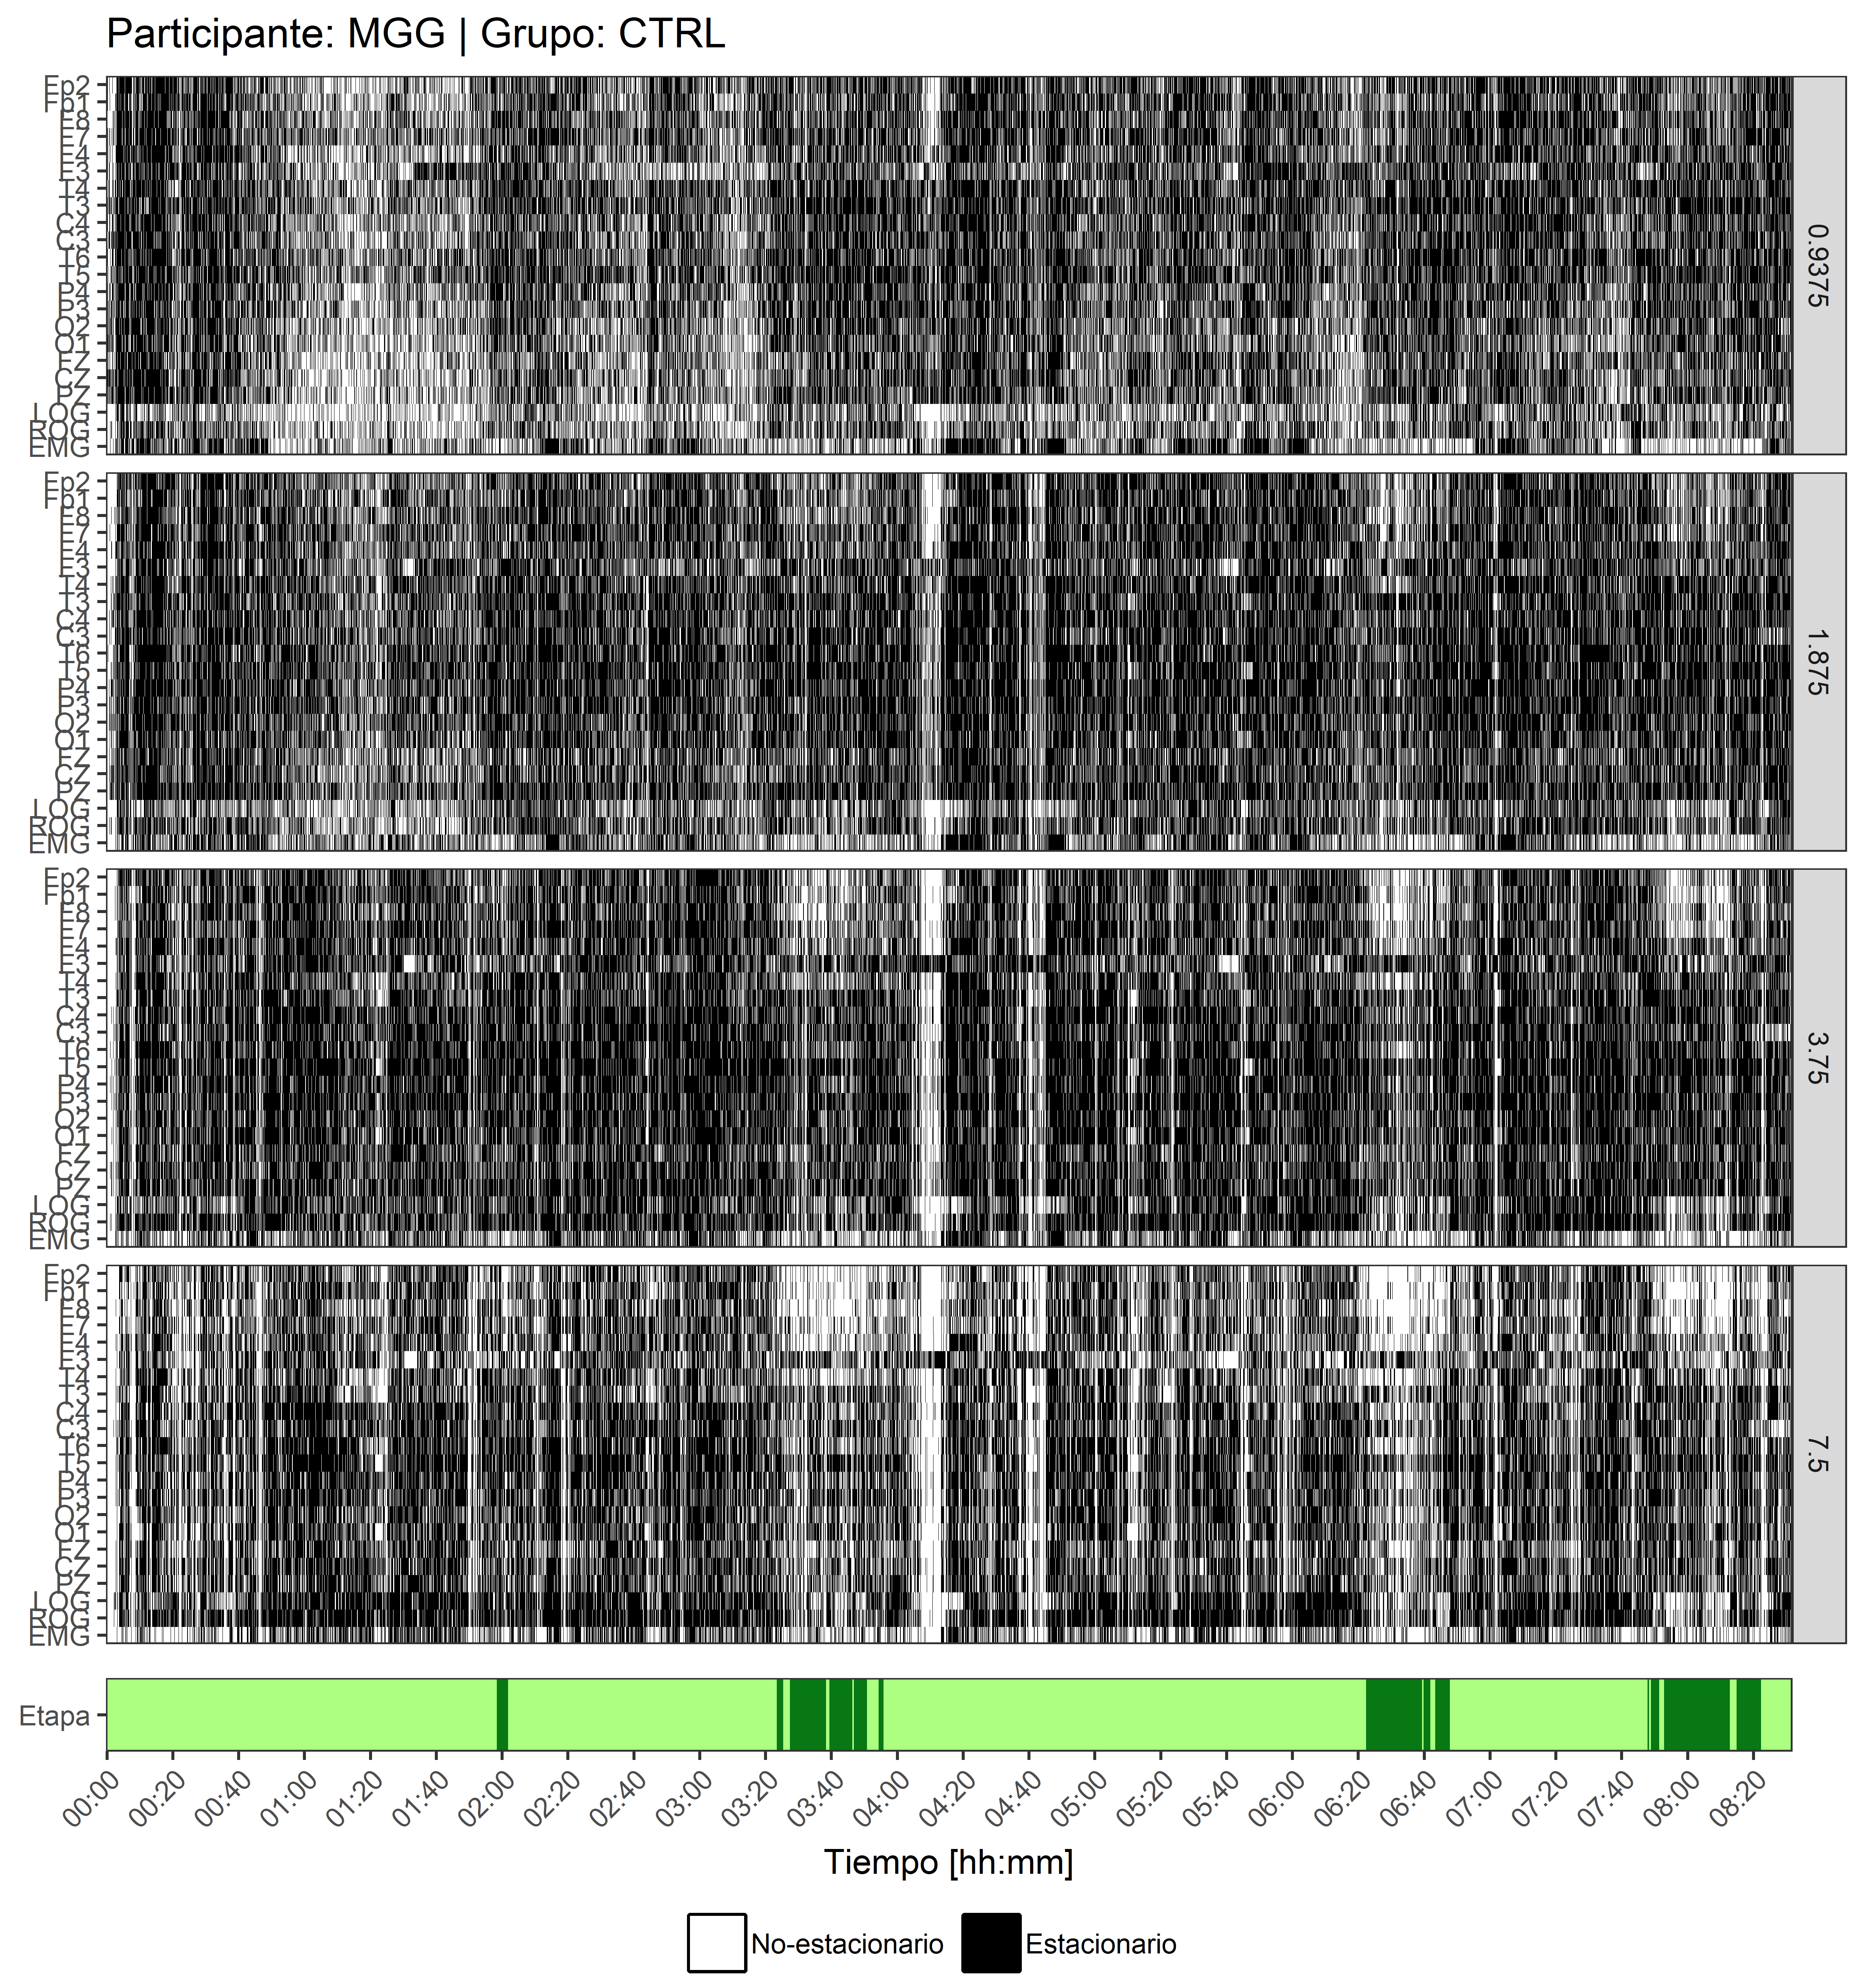
\includegraphics[width=\linewidth]
{./scripts_graf_res/MGG_patrones_1.png}
\caption[Distribución en el tiempo de las ventanas clasificadas como estacionarias, considerando diferentes tamaños de ventana]{Distribución en el tiempo de las ventanas clasificadas como estacionarias, considerando diferentes tamaños de ventana. 
Cada ventana fue representada en una cuadrícula según su derivación (margen izquierdo) y momento (margen inferior) de procedencia; posteriormente fue \textit{coloreada} según su clasificación como estacionaria.
Dado que la clasificación de estacionariedad se repitió usando diversos tamaños de ventana, éstos se indican en el margen derecho.
En la parte inferior se representan las mismas épocas en su clasificación según etapa de sueño.}
\end{figure}
\begin{figure}
\centering
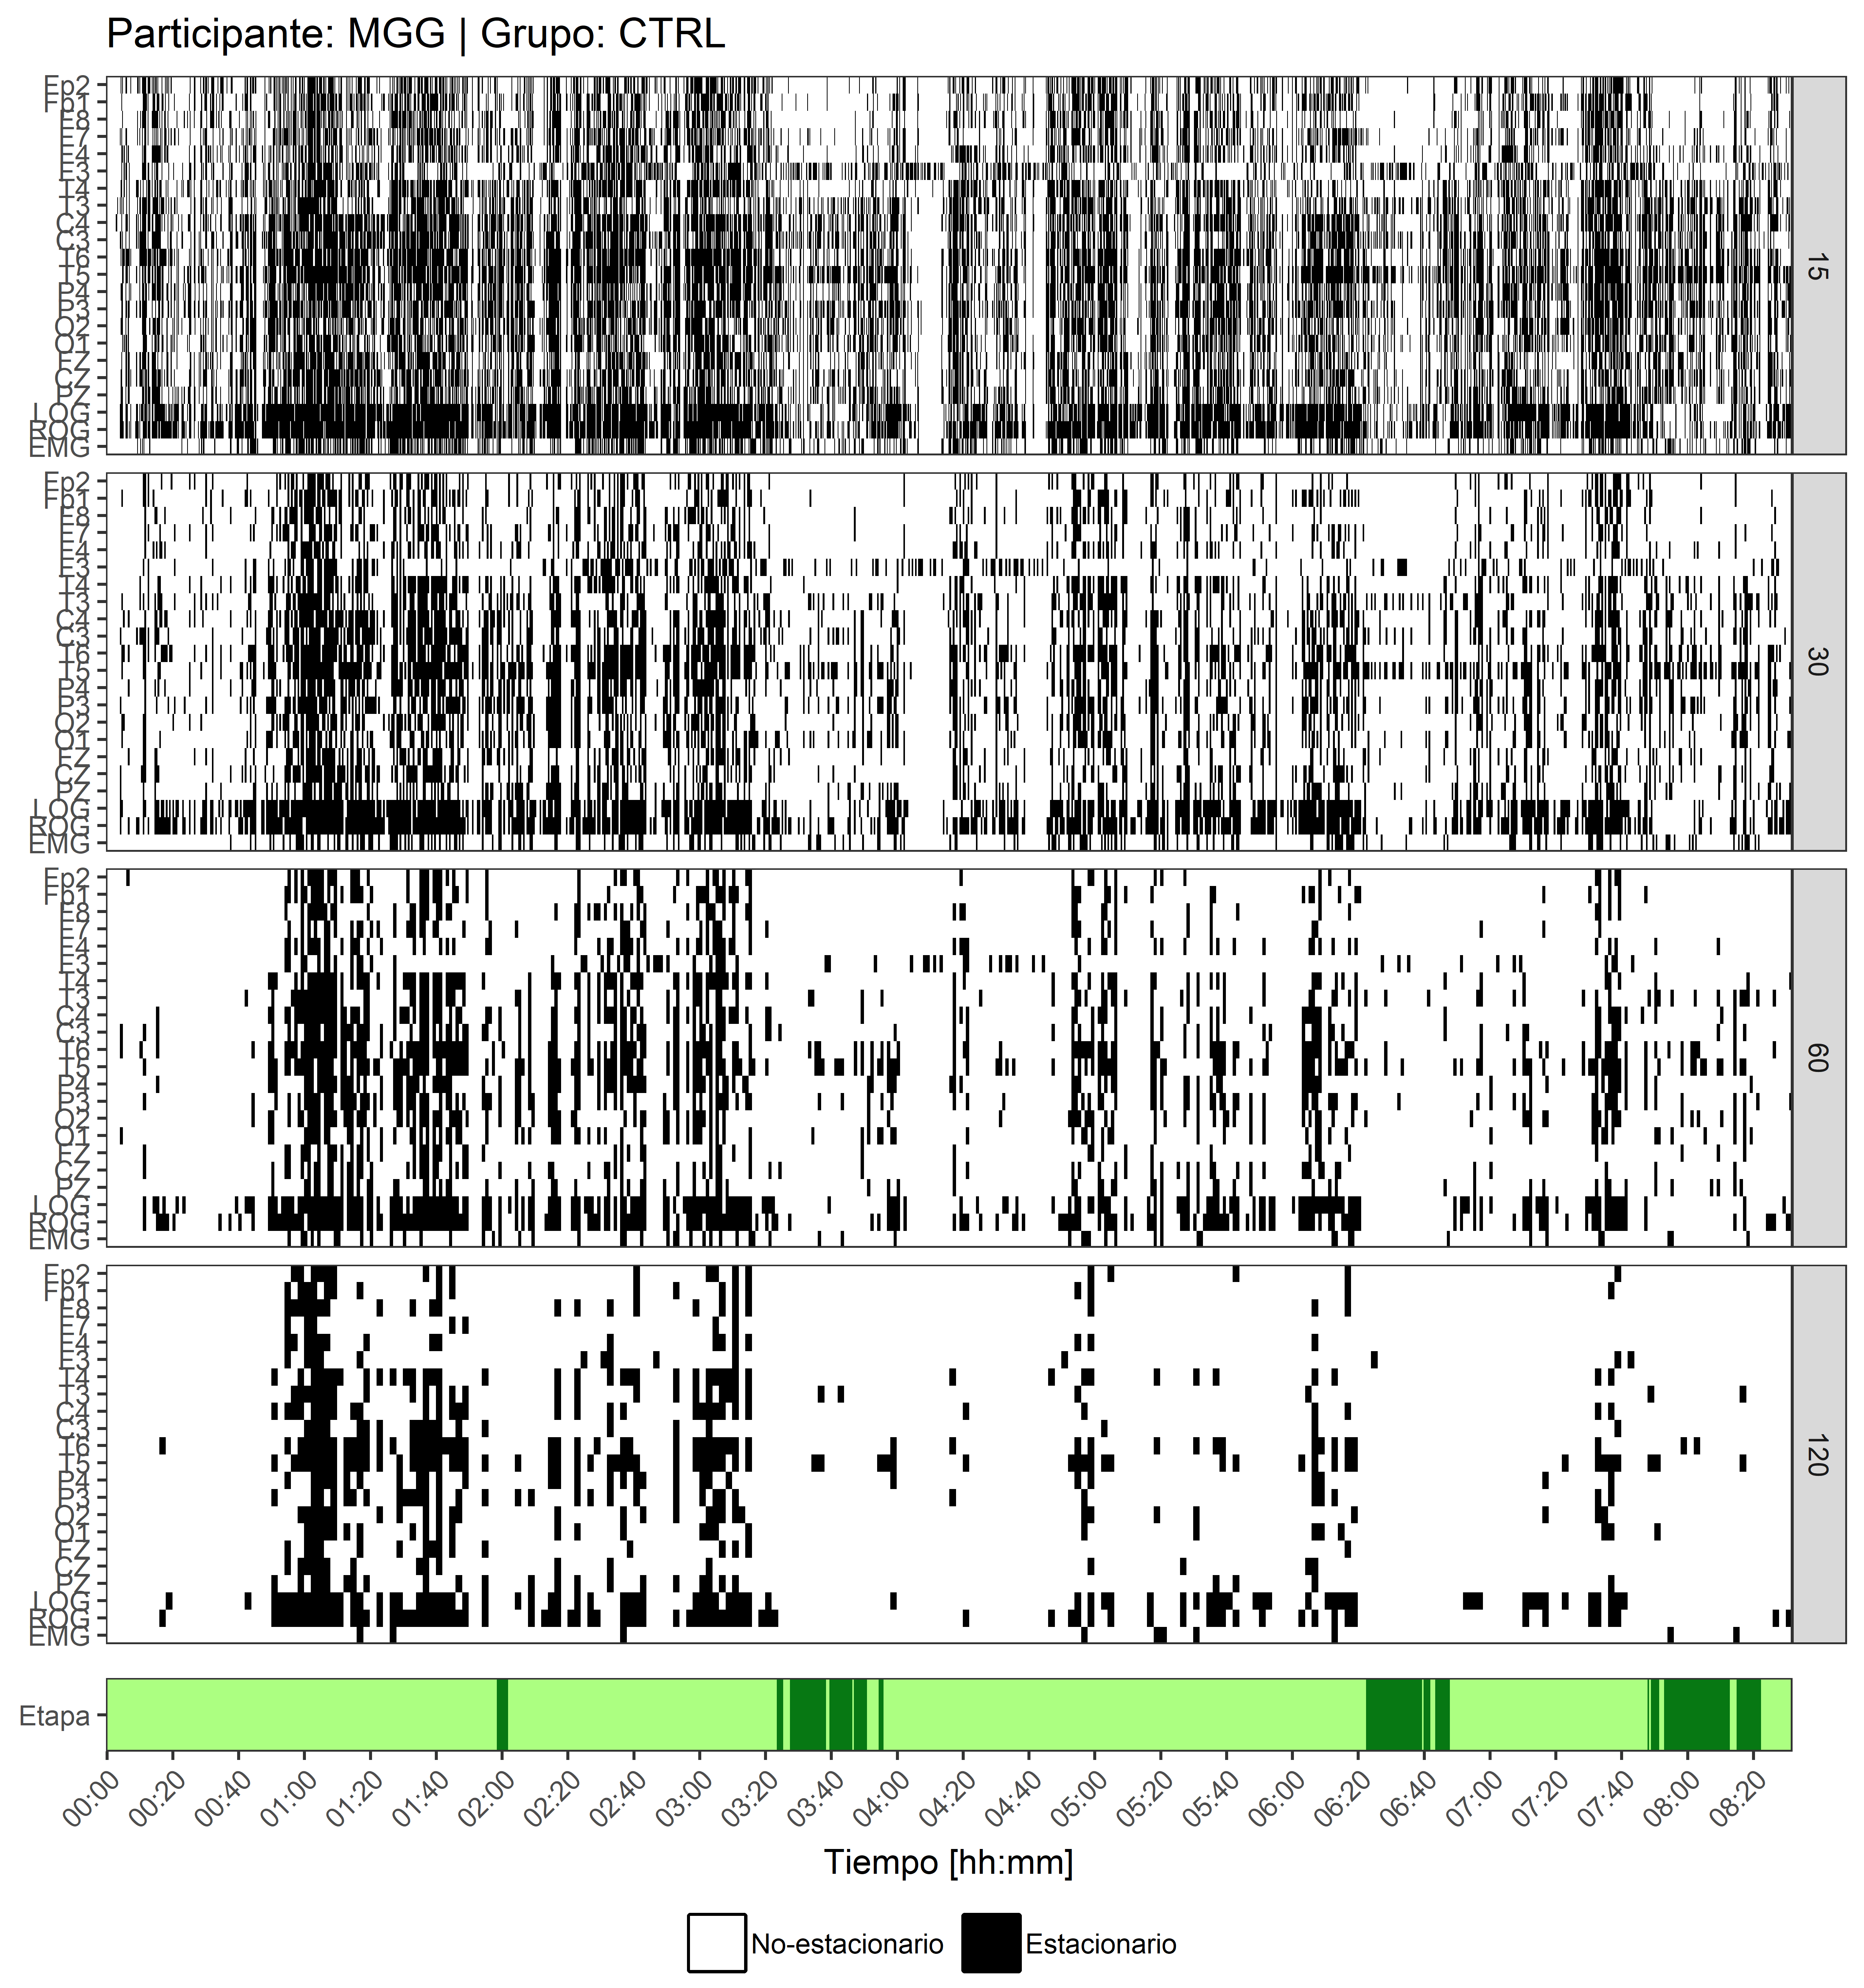
\includegraphics[width=\linewidth]
{./scripts_graf_res/MGG_patrones_2.png}
\caption[Distribución en el tiempo de las ventanas clasificadas como estacionarias, considerando diferentes tamaños de ventana]{Distribución en el tiempo de las ventanas clasificadas como estacionarias, considerando diferentes tamaños de ventana. 
Cada ventana fue representada en una cuadrícula según su derivación (margen izquierdo) y momento (margen inferior) de procedencia; posteriormente fue \textit{coloreada} según su clasificación como estacionaria.
Dado que la clasificación de estacionariedad se repitió usando diversos tamaños de ventana, éstos se indican en el margen derecho.
En la parte inferior se representan las mismas épocas en su clasificación según etapa de sueño.}
\end{figure}


\begin{figure}
\centering
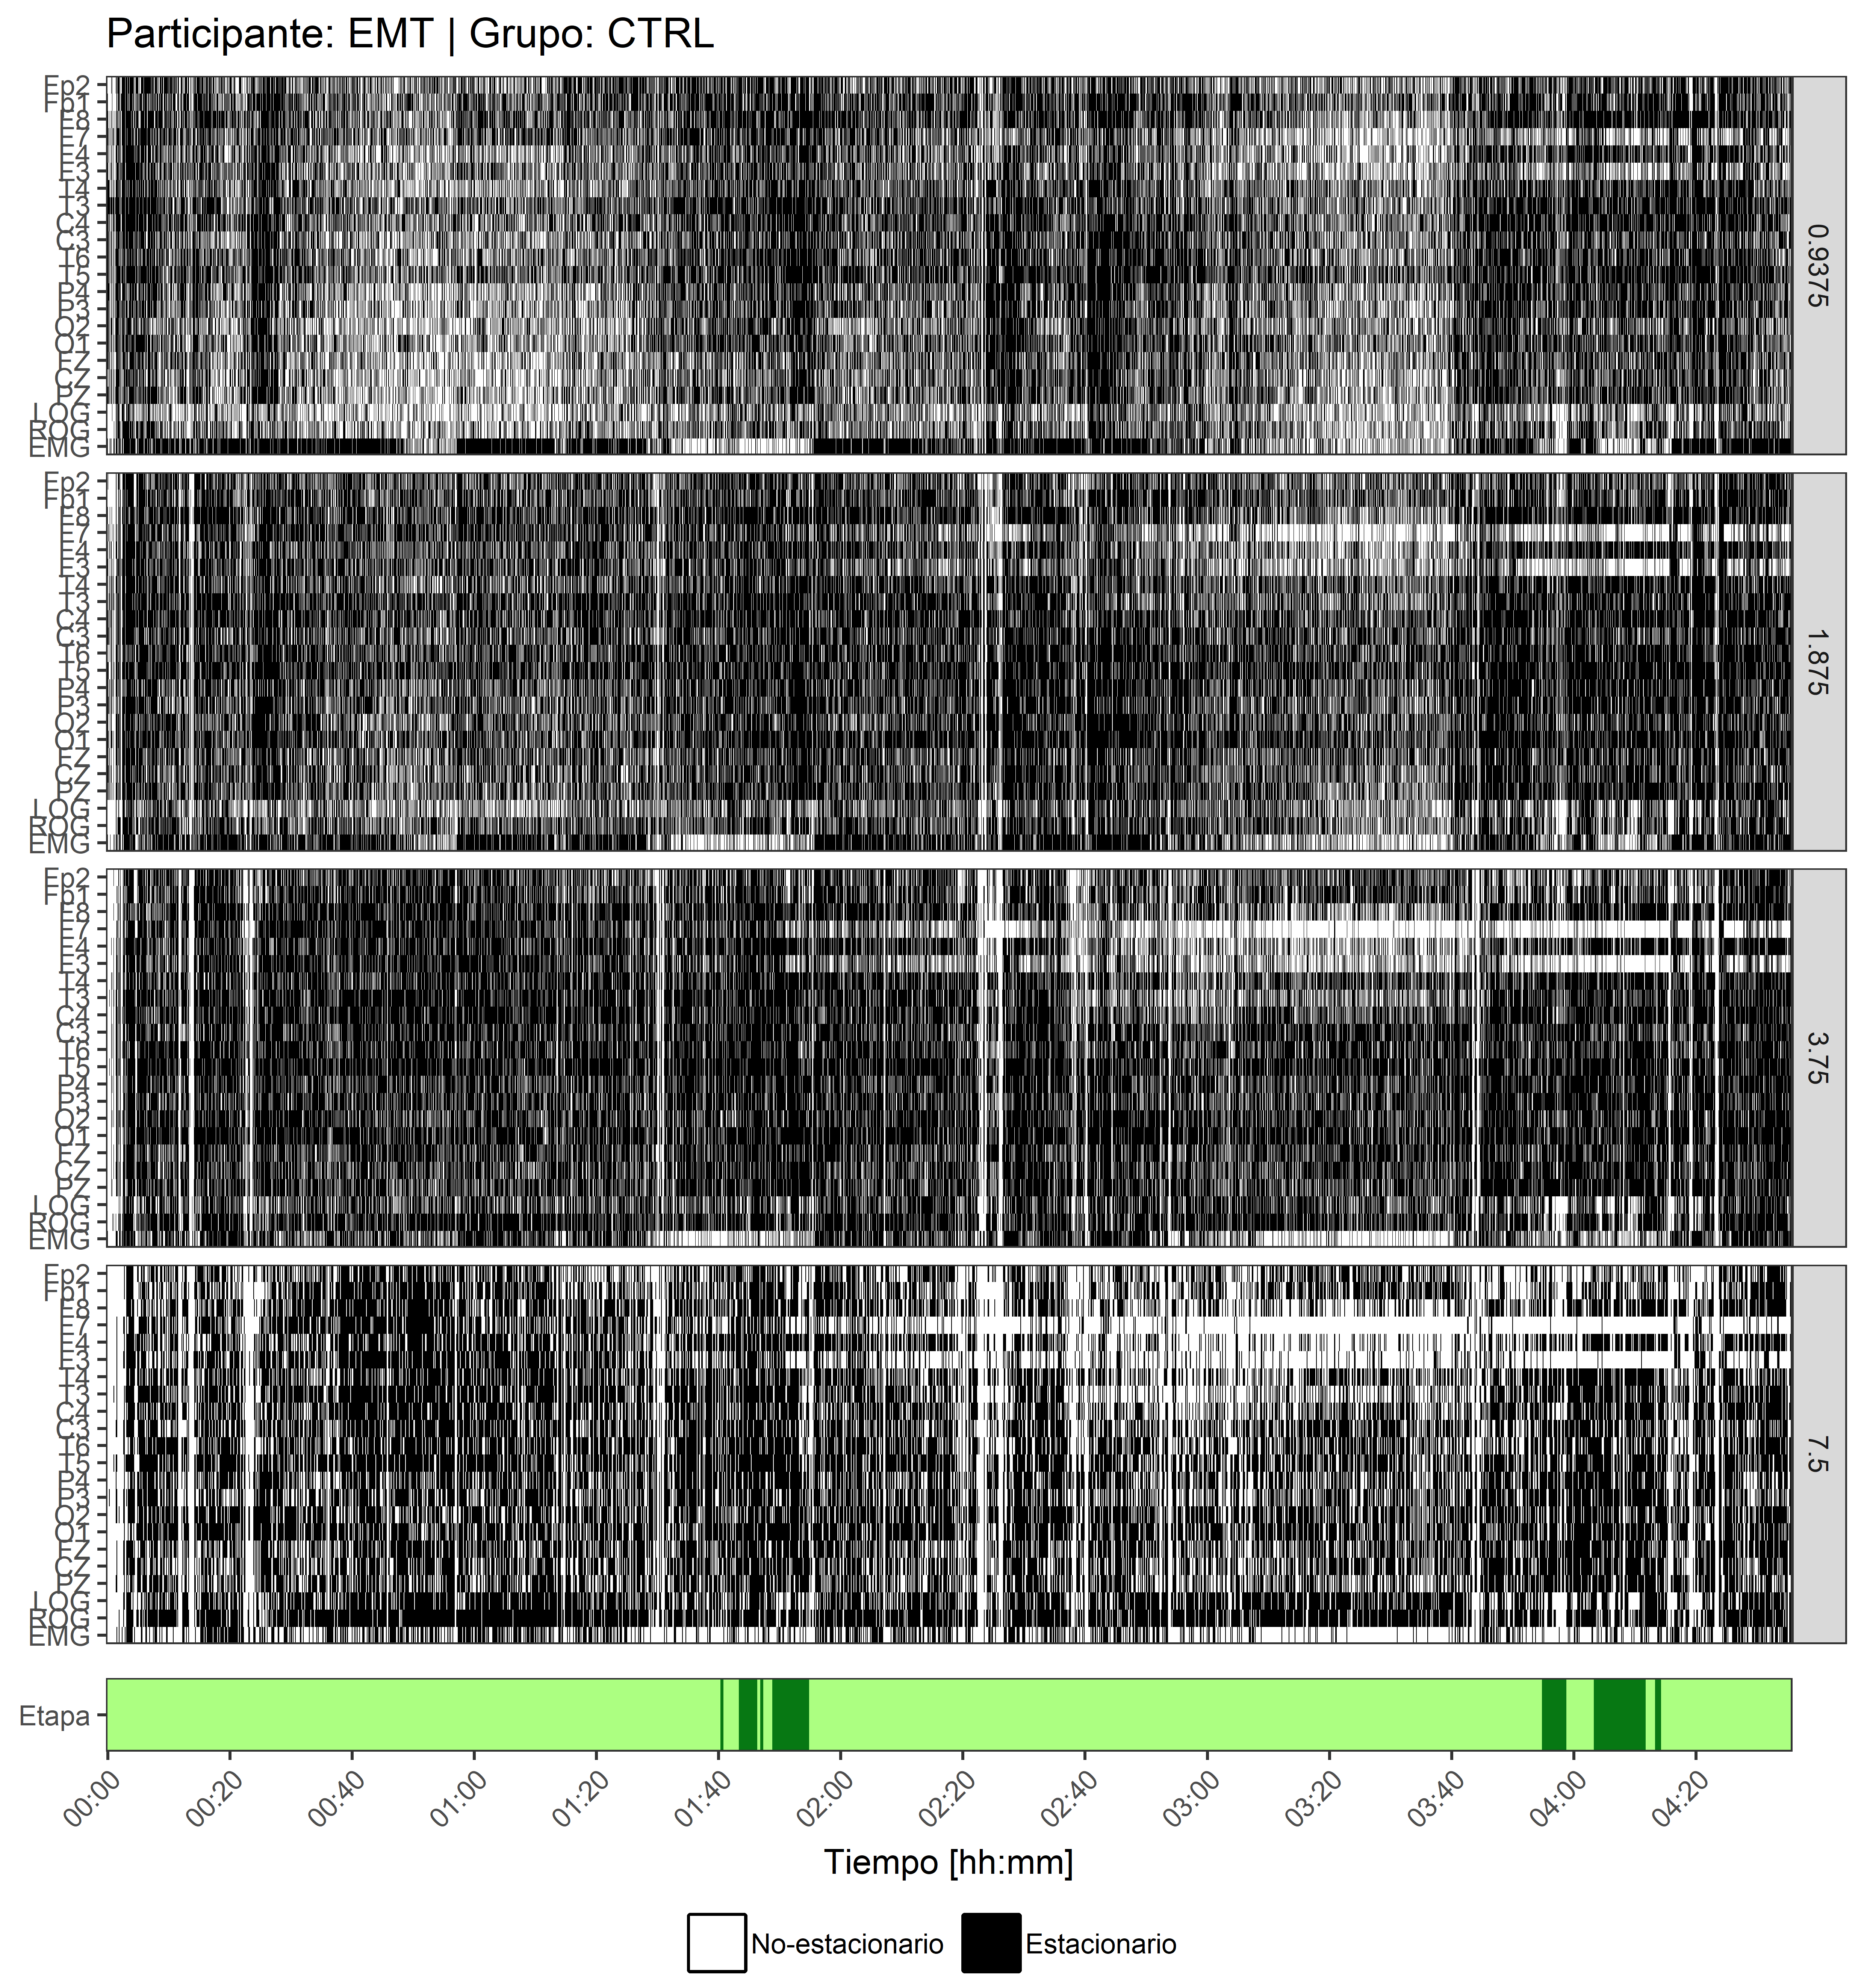
\includegraphics[width=\linewidth]
{./scripts_graf_res/EMT_patrones_1.png}
\caption[Distribución en el tiempo de las ventanas clasificadas como estacionarias, considerando diferentes tamaños de ventana]{Distribución en el tiempo de las ventanas clasificadas como estacionarias, considerando diferentes tamaños de ventana. 
Cada ventana fue representada en una cuadrícula según su derivación (margen izquierdo) y momento (margen inferior) de procedencia; posteriormente fue \textit{coloreada} según su clasificación como estacionaria.
Dado que la clasificación de estacionariedad se repitió usando diversos tamaños de ventana, éstos se indican en el margen derecho.
En la parte inferior se representan las mismas épocas en su clasificación según etapa de sueño.}
\end{figure}
\begin{figure}
\centering
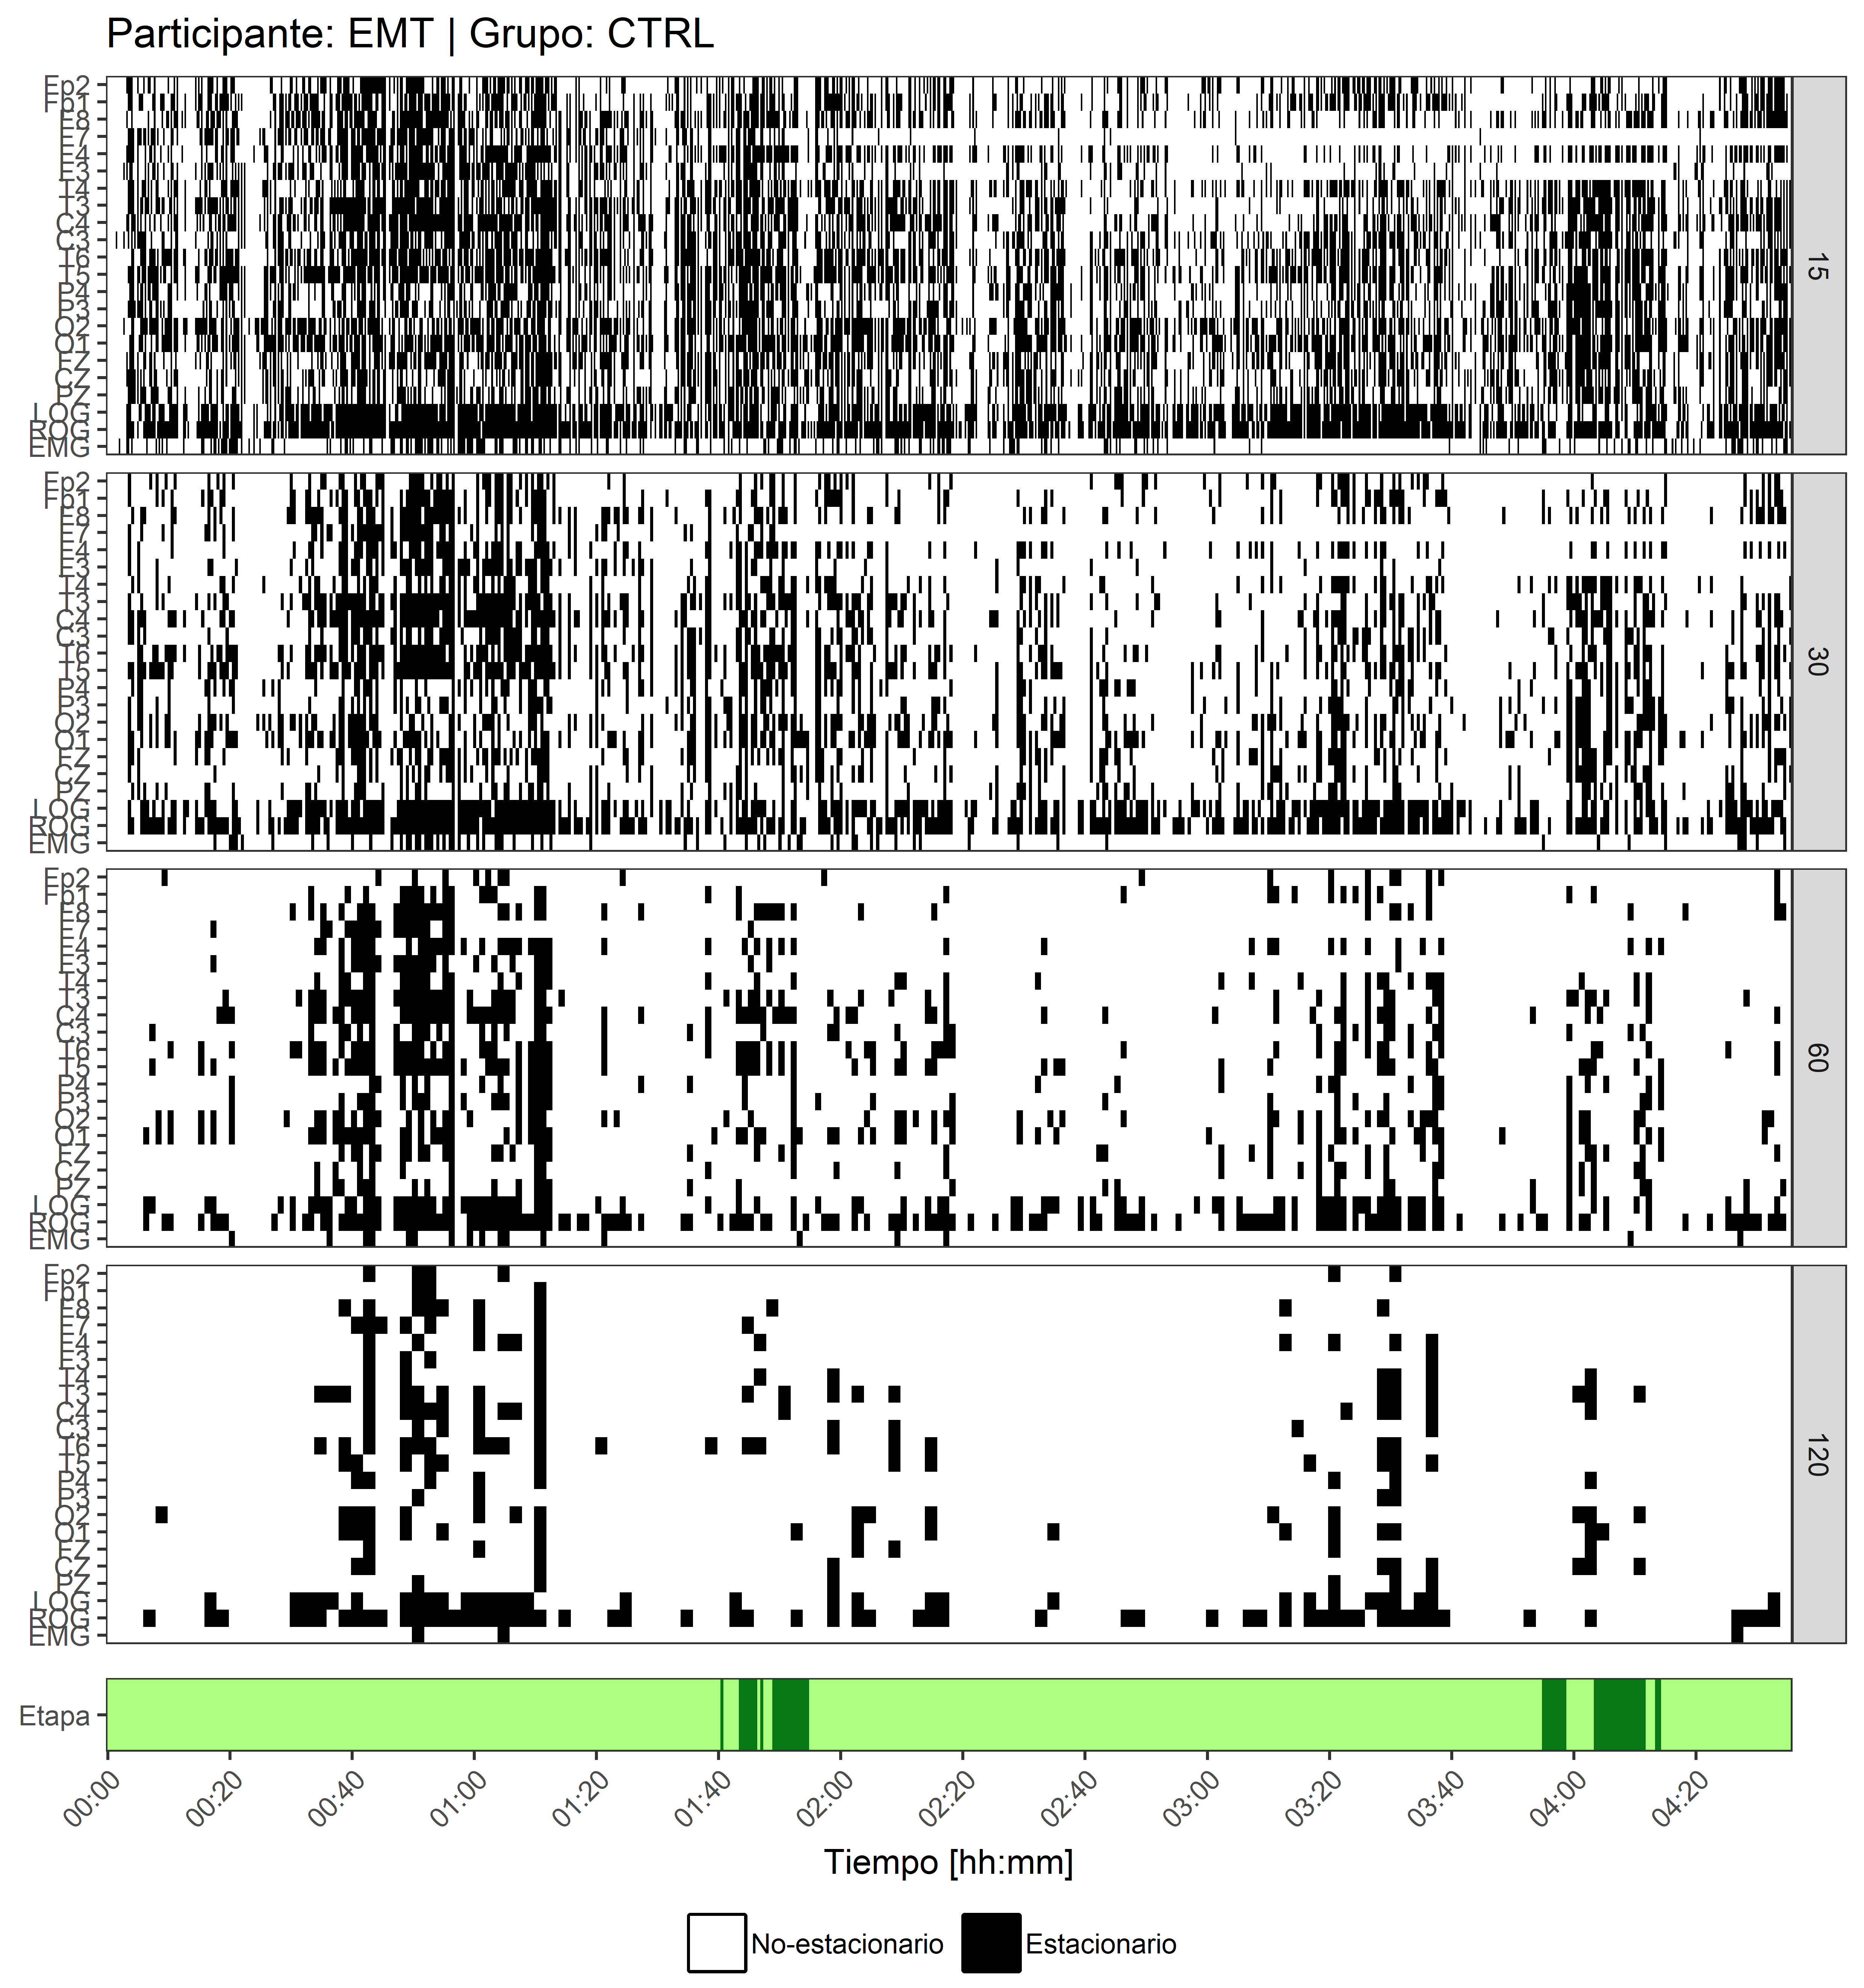
\includegraphics[width=\linewidth]
{./scripts_graf_res/EMT_patrones_2.png}
\caption[Distribución en el tiempo de las ventanas clasificadas como estacionarias, considerando diferentes tamaños de ventana]{Distribución en el tiempo de las ventanas clasificadas como estacionarias, considerando diferentes tamaños de ventana. 
Cada ventana fue representada en una cuadrícula según su derivación (margen izquierdo) y momento (margen inferior) de procedencia; posteriormente fue \textit{coloreada} según su clasificación como estacionaria.
Dado que la clasificación de estacionariedad se repitió usando diversos tamaños de ventana, éstos se indican en el margen derecho.
En la parte inferior se representan las mismas épocas en su clasificación según etapa de sueño.}
\end{figure}


\begin{figure}
\centering
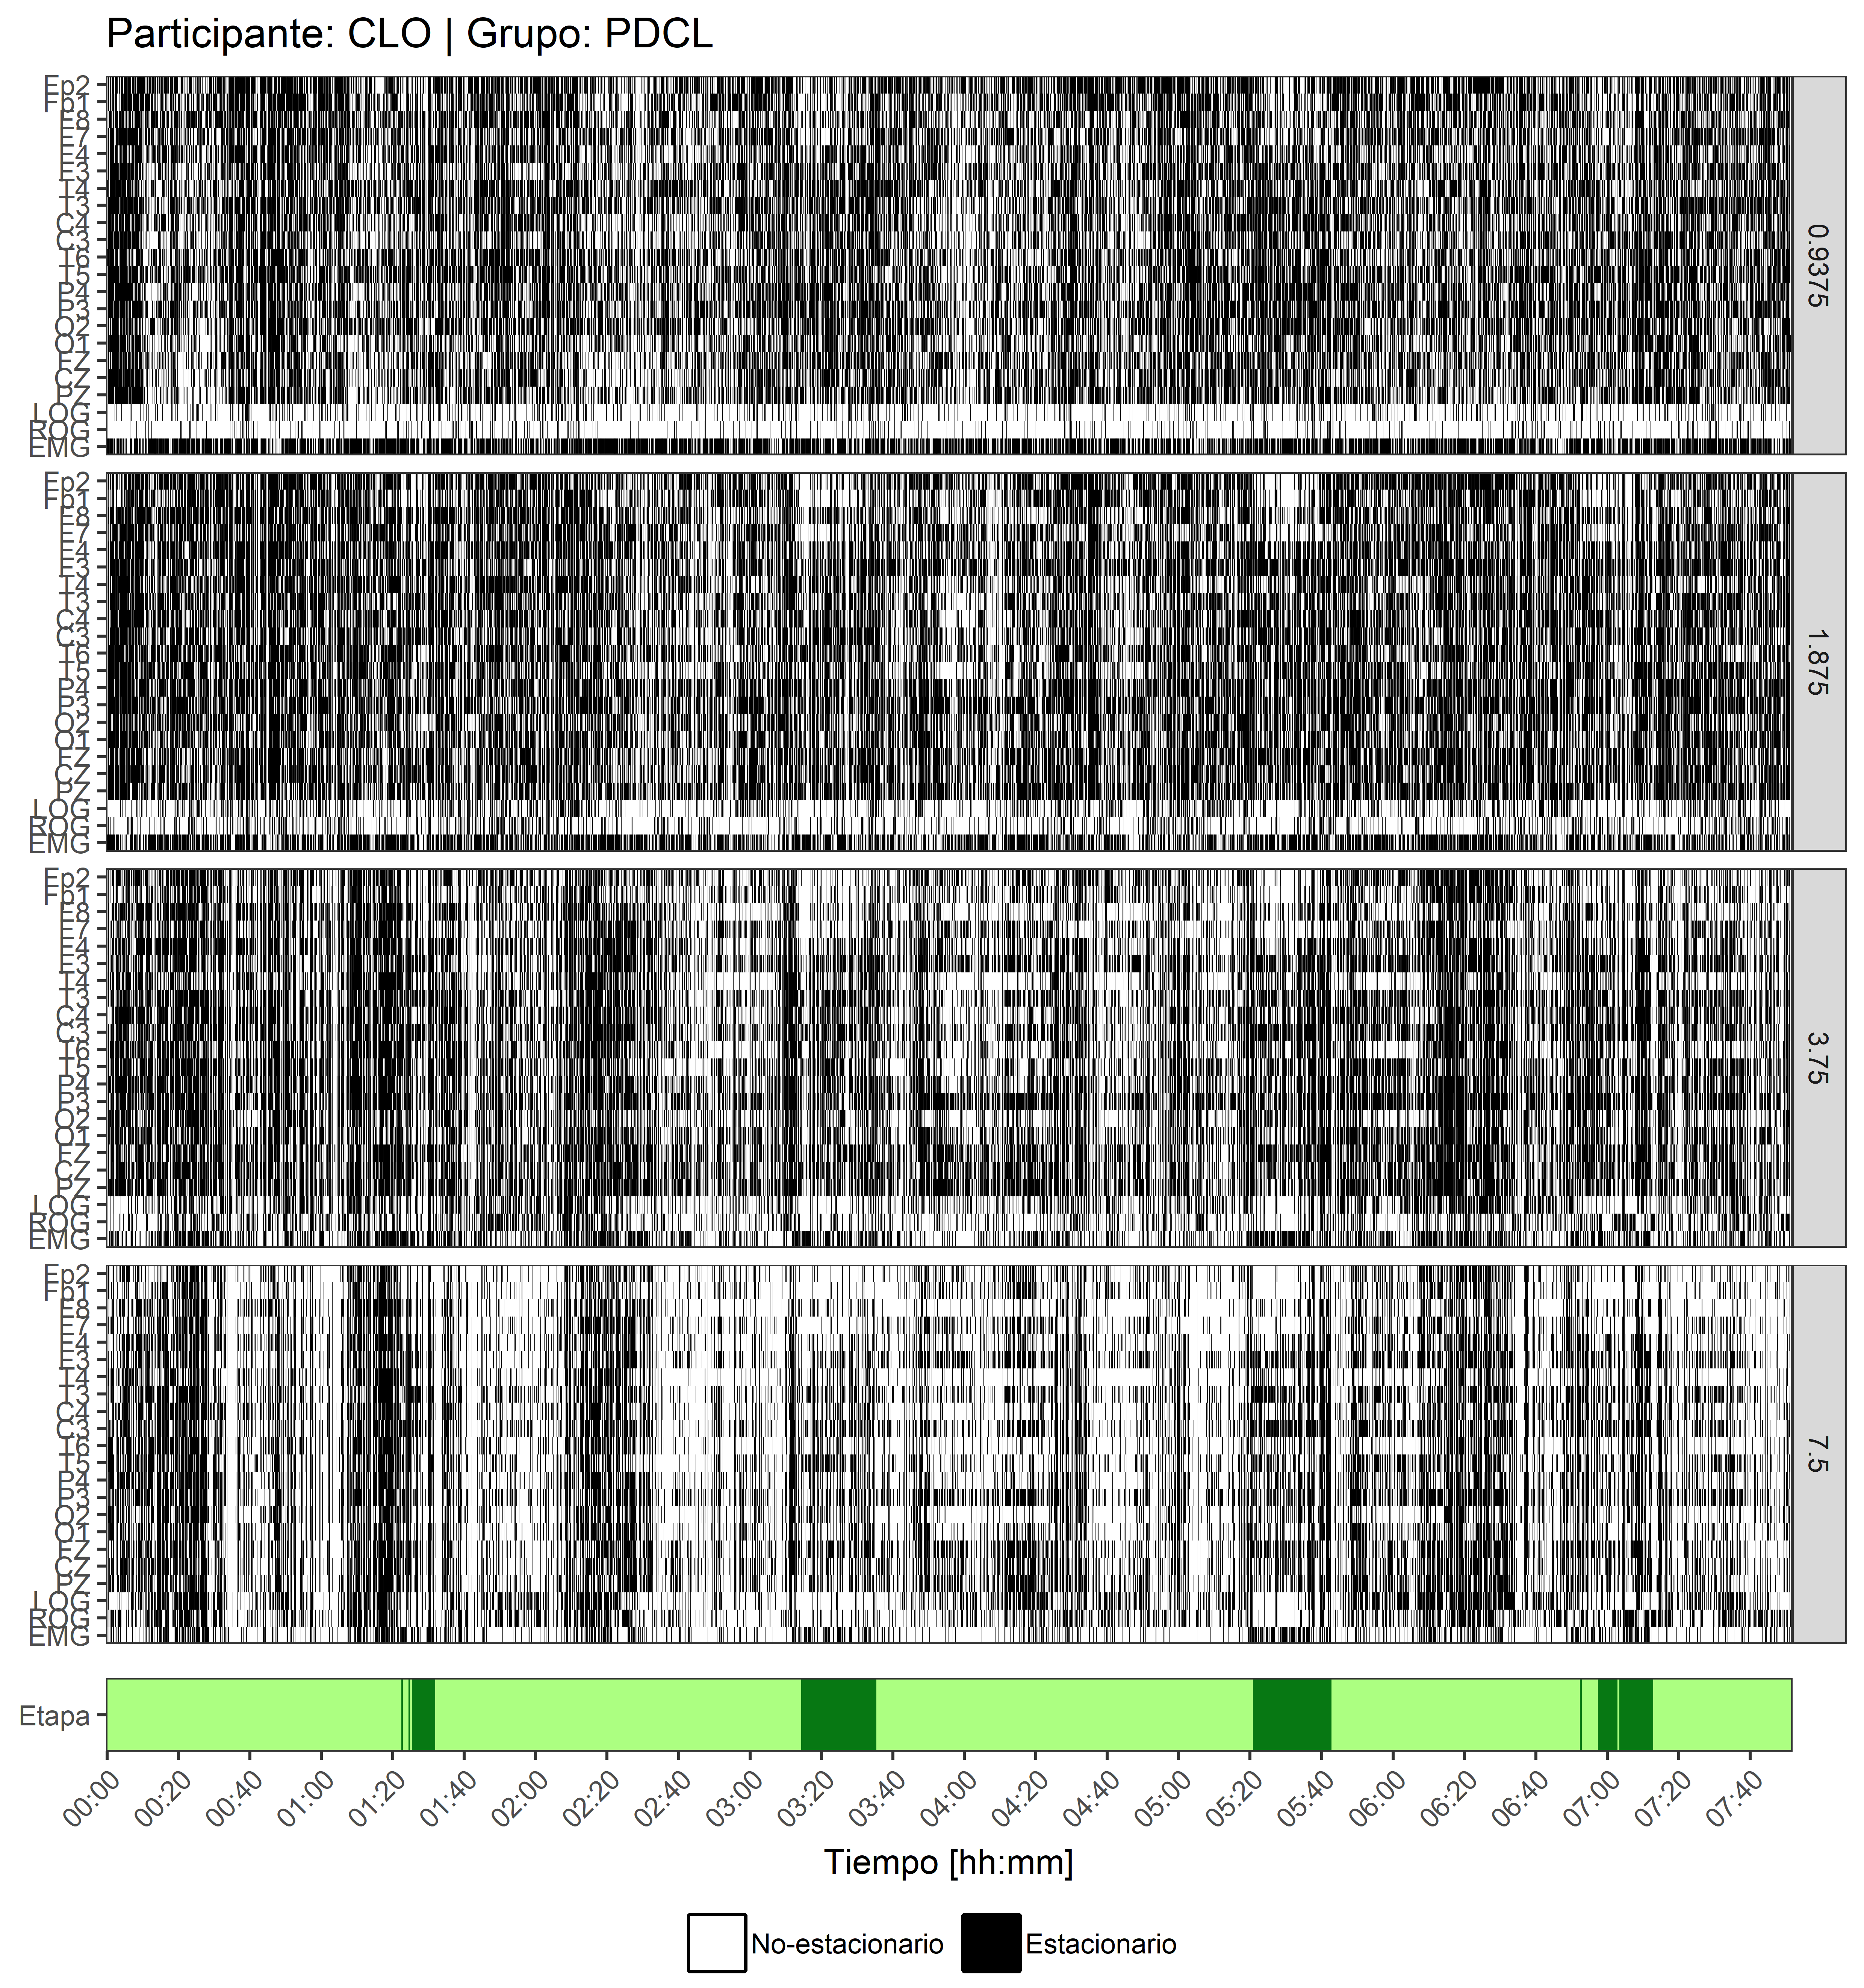
\includegraphics[width=\linewidth]
{./scripts_graf_res/CLO_patrones_1.png}
\caption[Distribución en el tiempo de las ventanas clasificadas como estacionarias, considerando diferentes tamaños de ventana]{Distribución en el tiempo de las ventanas clasificadas como estacionarias, considerando diferentes tamaños de ventana. 
Cada ventana fue representada en una cuadrícula según su derivación (margen izquierdo) y momento (margen inferior) de procedencia; posteriormente fue \textit{coloreada} según su clasificación como estacionaria.
Dado que la clasificación de estacionariedad se repitió usando diversos tamaños de ventana, éstos se indican en el margen derecho.
En la parte inferior se representan las mismas épocas en su clasificación según etapa de sueño.}
\end{figure}
\begin{figure}
\centering
\includegraphics[width=\linewidth]
{./scripts_graf_res/CLO_patrones_2.png}
\caption[Distribución en el tiempo de las ventanas clasificadas como estacionarias, considerando diferentes tamaños de ventana]{Distribución en el tiempo de las ventanas clasificadas como estacionarias, considerando diferentes tamaños de ventana. 
Cada ventana fue representada en una cuadrícula según su derivación (margen izquierdo) y momento (margen inferior) de procedencia; posteriormente fue \textit{coloreada} según su clasificación como estacionaria.
Dado que la clasificación de estacionariedad se repitió usando diversos tamaños de ventana, éstos se indican en el margen derecho.
En la parte inferior se representan las mismas épocas en su clasificación según etapa de sueño.}
\end{figure}


\begin{figure}
\centering
\includegraphics[width=\linewidth]
{./scripts_graf_res/RLO_patrones_1.png}
\caption[Distribución en el tiempo de las ventanas clasificadas como estacionarias, considerando diferentes tamaños de ventana]{Distribución en el tiempo de las ventanas clasificadas como estacionarias, considerando diferentes tamaños de ventana. 
Cada ventana fue representada en una cuadrícula según su derivación (margen izquierdo) y momento (margen inferior) de procedencia; posteriormente fue \textit{coloreada} según su clasificación como estacionaria.
Dado que la clasificación de estacionariedad se repitió usando diversos tamaños de ventana, éstos se indican en el margen derecho.
En la parte inferior se representan las mismas épocas en su clasificación según etapa de sueño.}
\end{figure}
\begin{figure}
\centering
\includegraphics[width=\linewidth]
{./scripts_graf_res/RLO_patrones_2.png}
\caption[Distribución en el tiempo de las ventanas clasificadas como estacionarias, considerando diferentes tamaños de ventana]{Distribución en el tiempo de las ventanas clasificadas como estacionarias, considerando diferentes tamaños de ventana. 
Cada ventana fue representada en una cuadrícula según su derivación (margen izquierdo) y momento (margen inferior) de procedencia; posteriormente fue \textit{coloreada} según su clasificación como estacionaria.
Dado que la clasificación de estacionariedad se repitió usando diversos tamaños de ventana, éstos se indican en el margen derecho.
En la parte inferior se representan las mismas épocas en su clasificación según etapa de sueño.}
\end{figure}


\begin{figure}
\centering
\includegraphics[width=\linewidth]
{./scripts_graf_res/JGZ_patrones_1.png}
\caption[Distribución en el tiempo de las ventanas clasificadas como estacionarias, considerando diferentes tamaños de ventana]{Distribución en el tiempo de las ventanas clasificadas como estacionarias, considerando diferentes tamaños de ventana. 
Cada ventana fue representada en una cuadrícula según su derivación (margen izquierdo) y momento (margen inferior) de procedencia; posteriormente fue \textit{coloreada} según su clasificación como estacionaria.
Dado que la clasificación de estacionariedad se repitió usando diversos tamaños de ventana, éstos se indican en el margen derecho.
En la parte inferior se representan las mismas épocas en su clasificación según etapa de sueño.}
\end{figure}
\begin{figure}
\centering
\includegraphics[width=\linewidth]
{./scripts_graf_res/JGZ_patrones_2.png}
\caption[Distribución en el tiempo de las ventanas clasificadas como estacionarias, considerando diferentes tamaños de ventana]{Distribución en el tiempo de las ventanas clasificadas como estacionarias, considerando diferentes tamaños de ventana. 
Cada ventana fue representada en una cuadrícula según su derivación (margen izquierdo) y momento (margen inferior) de procedencia; posteriormente fue \textit{coloreada} según su clasificación como estacionaria.
Dado que la clasificación de estacionariedad se repitió usando diversos tamaños de ventana, éstos se indican en el margen derecho.
En la parte inferior se representan las mismas épocas en su clasificación según etapa de sueño.}
\end{figure}


\begin{figure}
\centering
\includegraphics[width=\linewidth]
{./scripts_graf_res/AEFP_patrones_1.png}
\caption[Distribución en el tiempo de las ventanas clasificadas como estacionarias, considerando diferentes tamaños de ventana]{Distribución en el tiempo de las ventanas clasificadas como estacionarias, considerando diferentes tamaños de ventana. 
Cada ventana fue representada en una cuadrícula según su derivación (margen izquierdo) y momento (margen inferior) de procedencia; posteriormente fue \textit{coloreada} según su clasificación como estacionaria.
Dado que la clasificación de estacionariedad se repitió usando diversos tamaños de ventana, éstos se indican en el margen derecho.
En la parte inferior se representan las mismas épocas en su clasificación según etapa de sueño.}
\end{figure}
\begin{figure}
\centering
\includegraphics[width=\linewidth]
{./scripts_graf_res/AEFP_patrones_2.png}
\caption[Distribución en el tiempo de las ventanas clasificadas como estacionarias, considerando diferentes tamaños de ventana]{Distribución en el tiempo de las ventanas clasificadas como estacionarias, considerando diferentes tamaños de ventana. 
Cada ventana fue representada en una cuadrícula según su derivación (margen izquierdo) y momento (margen inferior) de procedencia; posteriormente fue \textit{coloreada} según su clasificación como estacionaria.
Dado que la clasificación de estacionariedad se repitió usando diversos tamaños de ventana, éstos se indican en el margen derecho.
En la parte inferior se representan las mismas épocas en su clasificación según etapa de sueño.}
\end{figure}


\begin{figure}
\centering
\includegraphics[width=\linewidth]
{./scripts_graf_res/PCM_patrones_1.png}
\caption[Distribución en el tiempo de las ventanas clasificadas como estacionarias, considerando diferentes tamaños de ventana]{Distribución en el tiempo de las ventanas clasificadas como estacionarias, considerando diferentes tamaños de ventana. 
Cada ventana fue representada en una cuadrícula según su derivación (margen izquierdo) y momento (margen inferior) de procedencia; posteriormente fue \textit{coloreada} según su clasificación como estacionaria.
Dado que la clasificación de estacionariedad se repitió usando diversos tamaños de ventana, éstos se indican en el margen derecho.
En la parte inferior se representan las mismas épocas en su clasificación según etapa de sueño.}
\end{figure}
\begin{figure}
\centering
\includegraphics[width=\linewidth]
{./scripts_graf_res/PCM_patrones_2.png}
\caption[Distribución en el tiempo de las ventanas clasificadas como estacionarias, considerando diferentes tamaños de ventana]{Distribución en el tiempo de las ventanas clasificadas como estacionarias, considerando diferentes tamaños de ventana. 
Cada ventana fue representada en una cuadrícula según su derivación (margen izquierdo) y momento (margen inferior) de procedencia; posteriormente fue \textit{coloreada} según su clasificación como estacionaria.
Dado que la clasificación de estacionariedad se repitió usando diversos tamaños de ventana, éstos se indican en el margen derecho.
En la parte inferior se representan las mismas épocas en su clasificación según etapa de sueño.}
\end{figure}

%%%%%%%%%%%%%%%%%%%%%%%%%%%%%%%%%%%%%%%%%%%%%%%%%

%\begin{figure}
%\Large{\textbf{Patrones visuales}}\\
%\includegraphics[width=0.95\textwidth]
%{./img_ejemplos/zoom_VCR.pdf}
%\caption{Test}
%\label{test1}
%\end{figure}
%
%\begin{figure}
%\includegraphics[width=0.95\textwidth]
%{./img_ejemplos/zoom_MJH.pdf}
%\caption{Test}
%\label{test2}
%\end{figure}
%
%\begin{figure}
%\includegraphics[width=0.95\textwidth]
%{./img_ejemplos/zoom_JAE.pdf}
%\caption{Test}
%\label{test3}
%\end{figure}
%
%\begin{figure}
%\includegraphics[width=0.95\textwidth]
%{./img_ejemplos/zoom_GHA.pdf}
%\caption{Test}
%\label{test4}
%\end{figure}
%
%
%\begin{figure}
%\includegraphics[width=0.95\textwidth]
%{./img_ejemplos/zoom_MFGR.pdf}
%\caption{Test}
%\label{test5}
%\end{figure}

%%%%%%%%%%%%%%%%%%%%%%%%%%%%%%%%%%%%%%%%%%%%%%%%%%%%%%%%%%%%%%%%%%%%%%%%%%%%%%%%%%%%%%%%%%%%%%%%%%%%
%%%%%%%%%%%%%%%%%%%%%%%%%%%%%%%%%%%%%%%%%%%%%%%%%%%%%%%%%%%%%%%%%%%%%%%%%%%%%%%%%%%%%%%%%%%%%%%%%%%%
%%%%%%%%%%%%%%%%%%%%%%%%%%%%%%%%%%%%%%%%%%%%%%%%%%%%%%%%%%%%%%%%%%%%%%%%%%%%%%%%%%%%%%%%%%%%%%%%%%%%
%%%%%%%%%%%%%%%%%%%%%%%%%%%%%%%%%%%%%%%%%%%%%%%%%%%%%%%%%%%%%%%%%%%%%%%%%%%%%%%%%%%%%%%%%%%%%%%%%%%%